\documentclass[a4paper]{article} %tạo một bản báo cáo
\usepackage[utf8]{inputenc}
\usepackage[T5]{fontenc} %để sử dụng tiếng việt
\usepackage[fontsize=11pt]{scrextend} %set font=13pt
\linespread{1.2}
\usepackage[paperheight=29.7cm,paperwidth=21cm,right=2cm,left=1.8cm,top=2cm,bottom=2.5cm]{geometry}
\usepackage{amsmath, amssymb, txfonts}
\usepackage{listings}
\usepackage{tabularx}
\usepackage{array}
\usepackage{diagbox}
\usepackage{vhistory}
\usepackage{indentfirst}
\usepackage{multirow}
\usepackage{graphicx} %thư viện chèn ảnh
\usepackage{float} % set vị trí chèn ảnh
\usepackage{tikz} % thư viện tạo khung bìa
\usetikzlibrary{calc} % thư viện tikz
\renewcommand{\figurename}{\fontsize{12pt}{0pt}\selectfont \bfseries Hình}
\renewcommand{\listfigurename}{Danh mục hình ảnh}
\renewcommand{\listtablename}{Danh mục bảng}
\renewcommand{\thefigure}{\thesection.\arabic{figure}}
\usepackage{caption}
\usepackage{enumerate} % để tùy chỉnh itemize
\captionsetup[figure]{labelsep=space}
\newtheorem{theorem}{Định lý}[section]
\newtheorem{defn}{Định nghĩa}[section]
\newtheorem{vd}{Ví dụ}[section]
\newtheorem{proof}{Chứng minh}
\usepackage{adjustbox}
\usepackage{esint}
\usepackage{fancyhdr}
\usepackage[colorlinks=true, linkcolor=black, citecolor=black, urlcolor=blue]{hyperref}
\usepackage{placeins}
\usepackage{subcaption}
\usepackage{microtype}
\usepackage{booktabs}
\usepackage{longtable}
\usepackage{lastpage}
\usepackage{tcolorbox}
\usepackage{changepage}
\usepackage[vietnamese]{babel}
\usepackage[
backend=biber,
style=numeric,
sorting=ynt
]{biblatex}
\DeclareLanguageMapping{vietnamese}{english}

\newcommand{\StudentOneName}{Huỳnh Minh Tiến}
\newcommand{\StudentOneID}{2313425}
\newcommand{\StudentTwoName}{Nguyễn Ngọc Trúc Quỳnh}
\newcommand{\StudentTwoID}{2312912}
\newcommand{\StudentThreeName}{Nguyễn Đức Nghĩa}
\newcommand{\StudentThreeID}{2312266}
\newcommand{\StudentFourName}{Võ Tiến Nam}
\newcommand{\StudentFourID}{2312205}
\newcommand{\StudentFiveName}{Phạm Ngọc Tây}
\newcommand{\StudentFiveID}{2313063}
\newcommand{\StudentSixName}{Nguyễn Minh Thái}
\newcommand{\StudentSixID}{2313101}
\newcommand{\StudentSevenName}{Vũ Minh Châu}
\newcommand{\StudentSevenID}{2310339}
\newcommand{\StudentEightName}{Phan Đình Khang}
\newcommand{\StudentEightID}{2311459}

% \renewcommand\thesection{\Roman{section}.}            % 1, 2, 3
% \renewcommand\thesubsection{\arabic{subsection}/}        % a, b, c
% \renewcommand\thesubsubsection{\alph{subsubsection}/}% 1, 2, 3 (lại số nhỏ)

% --- Nhưng vẫn muốn figure/table/equation dùng số thường ---
\makeatletter
\renewcommand{\thefigure}{\arabic{section}.\arabic{subsection}.\arabic{figure}}
\renewcommand{\thetable}{\arabic{section}.\arabic{subsection}.\arabic{table}}
\renewcommand{\theequation}{\arabic{section}.\arabic{subsection}.\arabic{equation}}
% \geometry{left=3cm,right=2.5cm,top=2.5cm,bottom=2.5cm}
\captionsetup{font=small,labelfont=bf}

% Reset lại bộ đếm hình/bảng/phương trình mỗi khi qua section mới
\@addtoreset{figure}{subsection}
\@addtoreset{table}{subsection}
\@addtoreset{equation}{subsection}
\makeatother
\addbibresource{references.bib}

\setlength{\headheight}{40pt}
\pagestyle{fancy}
\fancyhead{} % clear all header fields
\fancyhead[L]{
 \begin{tabular}{rl}
    \begin{picture}(25,15)(0,0)
    \put(0,-8){
\includegraphics[width=8mm, height=8mm]{figures/common/hcmut_logo.png}}
    %\put(0,-8){\epsfig{width=10mm,figure=hcmut.eps}}
   \end{picture}&
	%\includegraphics[width=8mm, height=8mm]{01_logobachkhoa.png} & %
	\begin{tabular}{l}
		\textbf{\bf \ttfamily ĐẠI HỌC QUỐC GIA THÀNH PHỐ HỒ CHÍ MINH}\\
		\textbf{\bf \ttfamily TRƯỜNG ĐẠI HỌC BÁCH KHOA}
	\end{tabular} 	
 \end{tabular}
}
\fancyhead[R]{
	\begin{tabular}{l}
		\tiny \bf \\
		\tiny \bf 
	\end{tabular}  }
\fancyfoot{} % clear all footer fields
\fancyfoot[L]{\scriptsize \ttfamily Báo cáo Bài tập lớn - Môn: Kiến trúc phần mềm (CO3017)}
\fancyfoot[R]{\scriptsize \ttfamily Trang {\thepage}/\pageref{LastPage}}
\renewcommand{\headrulewidth}{0.3pt}
\renewcommand{\footrulewidth}{0.3pt}



\begin{document}
    \begin{titlepage}
        \begin{tikzpicture}[overlay,remember picture]
			\draw [line width=3pt]
			($ (current page.north west) + (2.0cm,-2.0cm) $)
			rectangle
			($ (current page.south east) + (-2.0cm,2.5cm) $);
			\draw [line width=0.5pt]
			($ (current page.north west) + (2.1cm,-2.1cm) $)
			rectangle
			($ (current page.south east) + (-2.1cm,2.6cm) $);
		\end{tikzpicture}
		\begin{center}
			\vspace{-6pt} \fontsize{13pt}{0pt}\selectfont ĐẠI HỌC QUỐC GIA THÀNH PHỐ HỒ CHÍ MINH \\
			\textbf{\fontsize{16pt}{0pt}\selectfont TRƯỜNG ĐẠI HỌC BÁCH KHOA}\\
            \textbf{\fontsize{16pt}{0pt}\selectfont KHOA KHOA HỌC VÀ KỸ THUẬT MÁY TÍNH}
			\vspace{1cm}
			\begin{figure}[H]
				\centering
				
\includegraphics[width=4.318cm,height=4.318cm]{figures/common/hcmut_logo.png}
			\end{figure}
			\vspace{0.5cm}
            \rule{0.7\linewidth}{1pt} \\[0.3cm] % Đường thẳng trên
			\textbf{\fontsize{16pt}{0pt}\selectfont BÁO CÁO BÀI TẬP LỚN}\\
			\textbf{\fontsize{16pt}{0pt}\selectfont MÔN: KIẾN TRÚC PHẦN MỀM (CO3017)}\\
                \vspace{0.5cm}
                \parbox{0.9\linewidth}{\centering\textbf{\fontsize{16pt}{20pt}\selectfont THIẾT KẾ KIẾN TRÚC CHO HỆ THỐNG CHẤM CÔNG VÀ KIỂM SOÁT RA VÀO BẰNG MÃ QR}}\\
            \vspace{0.5cm}
            \rule{0.7\linewidth}{1pt} \\[1cm] % Đường thẳng dưới
		\end{center}

    \begin{table}[h]
    \centering
        \begin{tabular}{rl}
        \hspace{3 cm}\textbf{GVHD}:
        & ThS. Lê Đình Thuận\\
        \textbf{Lớp}: & L01\\
        \textbf{Sinh viên thực hiện}: & \StudentOneName{} - \StudentOneID\\
        & \StudentTwoName{} - \StudentTwoID\\
        & \StudentThreeName{} - \StudentThreeID\\
        & \StudentFourName{} - \StudentFourID\\
        & \StudentFiveName{} - \StudentFiveID\\
        & \StudentSixName{} - \StudentSixID\\
        & \StudentSevenName{} - \StudentSevenID\\
        & \StudentEightName{} - \StudentEightID\\
        \end{tabular}
    \end{table}
        \begin{center}
			\fontsize{12pt}{0pt}\selectfont\ Thành phố Hồ Chí Minh, tháng \number\month\space năm \number\year\\
		\end{center}
    \end{titlepage}
    \cleardoublepage

    \begin{center}
        \fontsize{13pt}{0pt}\selectfont \textbf{DANH SÁCH THÀNH VIÊN} \\
        
    \end{center}
    \hspace{-1cm}

    \begin{table}[H]
        \centering
        \small
        \renewcommand{\arraystretch}{1.4}
        \setlength{\tabcolsep}{8pt}
        \begin{tabular}{|c|c|c|m{5cm}|>{\centering\arraybackslash}m{1.5cm}|}
            \hline
            \textbf{STT} & \textbf{Họ và tên} & \textbf{MSSV} & \textbf{Nhiệm vụ} & \textbf{\% Hoàn thành}\\
            \hline
            1 & \StudentOneName & \StudentOneID & Tổng hợp tài liệu và định dạng \LaTeX & 100 \\
            \hline
            2 & \StudentTwoName & \StudentTwoID & Phân tích miền nghiệp vụ và phong cách kiến trúc & 100 \\
            \hline
            3 & \StudentThreeName & \StudentThreeID & Thiết kế kiến trúc logic và nguyên tắc thiết kế & 100 \\
            \hline
            4 & \StudentFourName & \StudentFourID & Phân tích yêu cầu phi chức năng và đặc tính kiến trúc & 100 \\
            \hline
            5 & \StudentFiveName & \StudentFiveID & Thiết kế kiến trúc vật lý và các quyết định kiến trúc & 100 \\
            \hline
            6 & \StudentSixName & \StudentSixID & Thiết kế yêu cầu chức năng và đặc tả use-case & 100 \\
            \hline
            7 & \StudentSevenName & \StudentSevenID & Tổng hợp tài liệu và định dạng \LaTeX & 100 \\
            \hline
            8 & \StudentEightName & \StudentEightID & Bối cảnh và yêu cầu nghiệp vụ & 100 \\
            \hline
        \end{tabular}
    \end{table}
    \textbf{Ghi chú:} 


    \cleardoublepage
    \tableofcontents
    \cleardoublepage
    \phantomsection
    \addcontentsline{toc}{section}{Danh mục bảng}
    \listoftables
    \cleardoublepage
    \phantomsection
    \addcontentsline{toc}{section}{Danh mục hình ảnh}
    \listoffigures
    \cleardoublepage
    \begin{versionhistory}
        \vhEntry{1.0}{2026.10.19}{TienHM}{Tạo tài liệu}
        \vhEntry{1.1}{2026.10.21}{TienHM}{Bổ sung và chuẩn hóa yêu cầu chức năng FR-07--FR-28 về trạm cổng, chấm công, báo cáo, HR/Payroll, kiểm toán và quản trị hệ thống}
        \vhEntry{1.2}{2026.10.22}{TienHM}{Bổ sung yêu cầu phi chức năng theo 8 tiêu chí; chuẩn hóa cột ID, tiêu đề Mô tả và thuật ngữ cổng xoay}
        \vhEntry{1.3}{2026.10.23}{ChauVM}{Bổ sung phần 5, 6, 7, 8}
        \vhEntry{1.4}{2026.10.23}{TienHM}{Cấu trúc lại các phần để thống nhất nội dung sau khi phân tích}
        \vhEntry{1.5}{2026.11.15}{TienHM}{Tổ chức lại thư mục hình và quản lý mã nguồn báo cáo; Phần 2: bổ sung mã mục tiêu OBJ-01--OBJ-05, giả định A-04, A-05, rủi ro R-06; xác định HR/Payroll là nguồn dữ liệu nhân sự chính thức; thống nhất vai trò Giám sát sản xuất}
        \vhEntry{1.6}{2026.11.15}{TienHM}{Phần 3: chuẩn hóa yêu cầu chức năng theo mã QR động, đồng bộ nhân viên từ HR/Payroll và ngưỡng mất kết nối; bổ sung nhóm NFR Performance, NFR-SEC-05, NFR-SEC-06, NFR-AUD-05, NFR-MOD-01, NFR-SCA-01}
        \vhEntry{1.7}{2026.11.15}{TienHM}{Phần 4: cập nhật luồng nghiệp vụ, bổ sung bất biến INV-01--INV-11 và phân rã subdomain, vẽ lại lược đồ lớp; Phần 5: bổ sung đặc tính Modifiability và đánh đổi Availability -- Security}
        \vhEntry{1.8}{2026.11.15}{TienHM}{Tái cấu trúc Phần 6: so sánh và lựa chọn architecture style, xây dựng kiến trúc logic và kiến trúc vật lý theo từng bước, trình bày module views, component-and-connector views và allocation views; vẽ lại các hình theo chuẩn UML}
        \vhEntry{1.9}{2026.11.16}{TienHM}{Viết lại Phần 7 (ADR-01--ADR-08), bổ sung ADR-09 về đồng bộ nhân viên và ADR-10 về nền tảng công nghệ; tái cấu trúc Phần 8 thành bốn nhóm nguyên tắc DP-01--DP-17, mở rộng phần áp dụng SOLID kèm lược đồ lớp}
        \vhEntry{1.10}{2026.11.22}{NamVT}{Dựng bản nháp Mục 9.5 và 9.6 từ mã nguồn backend, hợp đồng OpenAPI và sitemap; bổ sung danh mục endpoint và các nội dung cần xác nhận sau tích hợp}
    \end{versionhistory}
    \cleardoublepage

    % DONE

    \section{Giới thiệu}

\textbf{Thiết kế kiến trúc phần mềm (Software Architecture Design)} là một giai đoạn quan trọng trong vòng đời phát triển phần mềm, đóng vai trò định hình cấu trúc tổng thể của hệ thống thông qua việc xác định các thành phần chính, trách nhiệm, mối quan hệ và cơ chế tương tác giữa chúng. Không chỉ là cơ sở định hướng cho quá trình thiết kế chi tiết và triển khai, kiến trúc phần mềm còn giúp chuyển hóa các yêu cầu nghiệp vụ thành một giải pháp kỹ thuật có tổ chức, nhất quán và phù hợp với mục tiêu của hệ thống. Đặc biệt, một kiến trúc được thiết kế tốt cần đáp ứng đồng thời các yêu cầu chức năng và phi chức năng như hiệu năng, tính bảo mật, độ tin cậy, khả năng mở rộng và khả năng bảo trì. Bên cạnh đó, việc xác định rõ ranh giới thành phần, các nguyên tắc thiết kế và những quyết định kiến trúc quan trọng giúp giảm sự phụ thuộc không cần thiết, hỗ trợ phối hợp giữa các nhóm phát triển, hạn chế rủi ro kỹ thuật và tối ưu chi phí thay đổi trong dài hạn. Vì vậy, thiết kế kiến trúc phần mềm không chỉ là nền tảng cho việc xây dựng một hệ thống đáp ứng yêu cầu hiện tại mà còn quyết định khả năng thích ứng, phát triển và duy trì chất lượng của hệ thống trong tương lai.

Trong khuôn khổ bài tập lớn môn Kiến trúc Phần mềm, nhóm thực hiện đề tài \textbf{Thiết kế kiến trúc cho hệ thống chấm công và kiểm soát ra vào bằng mã QR} được giả định cho Công ty Cổ phần Sản xuất TMC. Hệ thống được xây dựng nhằm hỗ trợ định danh nhân viên thông qua mã QR, kiểm soát quá trình ra vào tại các cổng, ghi nhận dữ liệu chấm công và cung cấp chức năng báo cáo, kiểm toán và tích hợp với hệ thống nhân sự của công ty. Trên cơ sở các yêu cầu nghiệp vụ và những ràng buộc kỹ thuật được xác định trong đề bài, nhóm tập trung phân tích bối cảnh hệ thống, xác định các đặc tính kiến trúc, đánh giá và lựa chọn phong cách kiến trúc phù hợp, xây dựng kiến trúc logic và kiến trúc vật lý, đồng thời xác lập các quyết định và nguyên tắc thiết kế cần thiết. Qua đó, nhóm hướng đến một kiến trúc đáp ứng các yêu cầu về hiệu năng, tính toàn vẹn dữ liệu, bảo mật và khả năng kiểm soát truy cập, làm nền tảng cho quá trình hoàn thiện thiết kế, triển khai và kiểm thử hệ thống ở các giai đoạn tiếp theo.

Bài tập lớn được triển khai theo hai cột mốc chính (Milestone), với phạm vi công việc được xác định theo từng giai đoạn. Cụ thể, \textbf{Milestone 1 (M1)} tập trung vào phân tích yêu cầu và thiết kế kiến trúc phần mềm, bao gồm mô tả bối cảnh hệ thống, xác định các yêu cầu chức năng và phi chức năng, lựa chọn phong cách kiến trúc, xây dựng kiến trúc logic và kiến trúc vật lý, đồng thời xác định các quyết định và nguyên tắc thiết kế. Tiếp theo, \textbf{Milestone 2 (M2)} hướng đến hiện thực hóa phiên bản MVP của hệ thống, đặc tả giao diện người dùng, hợp đồng API và chiến lược kiểm thử nhằm đánh giá mức độ đáp ứng các yêu cầu đã đề ra. Báo cáo này trình bày xuyên suốt cả phần thiết kế kiến trúc (M1) ở các Chương 2--8 và phần hiện thực hệ thống MVP (M2) ở Chương 9.

Báo cáo gồm các chương chính sau:
\begin{itemize}
    \item \textbf{Chương 2 – Nghiên cứu bối cảnh và phân tích nghiệp vụ:} Trình bày bối cảnh doanh nghiệp, mục tiêu và phạm vi hệ thống, các bên liên quan, ranh giới hệ thống, cùng các ràng buộc, giả định và rủi ro.
    \item \textbf{Chương 3 – Thiết kế yêu cầu hệ thống:} Đặc tả các yêu cầu chức năng theo nhóm nghiệp vụ và các yêu cầu phi chức năng, làm cơ sở đánh giá chất lượng và định hướng kiến trúc.
    \item \textbf{Chương 4 – Thiết kế mô hình miền nghiệp vụ:} Mô tả luồng nghiệp vụ chính, các thực thể và quan hệ giữa chúng; trình bày lược đồ lớp ở mức nghiệp vụ.
    \item \textbf{Chương 5 – Đặc tính kiến trúc hệ thống:} Phân tích các đặc tính kiến trúc, lựa chọn ba đặc tính dẫn dắt ưu tiên và đánh giá các đánh đổi.
    \item \textbf{Chương 6 – Cấu trúc kiến trúc hệ thống:} Phân tích architecture quantum, so sánh và lựa chọn architecture style, sau đó trình bày kiến trúc logic và kiến trúc vật lý.
    \item \textbf{Chương 7 – Quyết định kiến trúc hệ thống:} Tổng hợp và phân tích các quyết định kiến trúc về triển khai, xác thực QR, lưu trữ và đồng bộ giao dịch, tích hợp, tổ chức mã nguồn, bảo mật và quyền riêng tư.
    \item \textbf{Chương 8 – Nguyên lý thiết kế hệ thống:} Trình bày các nguyên tắc cấp kiến trúc, cách áp dụng SOLID, cohesion, coupling và tổ chức mã nguồn.
    \item \textbf{Chương 9 – Hiện thực hệ thống:} Trình bày phạm vi MVP, công nghệ và mô hình triển khai container hóa, cấu trúc mã nguồn, thiết kế chi tiết các module cốt lõi, hiện thực chức năng, danh mục màn hình giao diện (sitemap) và đặc tả hợp đồng API.
    \item \textbf{Phụ lục:} Bao gồm các sơ đồ use case và đặc tả bốn use case có ý nghĩa kiến trúc.
\end{itemize}

Nhóm xin chân thành cảm ơn ThS. Lê Đình Thuận đã tận tình giảng dạy, hướng dẫn và hỗ trợ nhóm trong suốt quá trình học tập môn Kiến trúc Phần mềm cũng như thực hiện bài tập lớn. Những kiến thức chuyên môn, định hướng và góp ý quý báu của thầy đã giúp nhóm hiểu rõ hơn về các nguyên lý thiết kế kiến trúc và vận dụng vào quá trình phân tích, xây dựng giải pháp cho hệ thống. Tuy nhiên, do kiến thức và kinh nghiệm thực tiễn còn hạn chế, báo cáo khó tránh khỏi những thiếu sót. Nhóm rất mong nhận được những ý kiến đóng góp từ thầy để hoàn thiện báo cáo và nâng cao kiến thức chuyên môn.
    \section{Nghiên cứu bối cảnh và phân tích nghiệp vụ}
\subsection{Bối cảnh doanh nghiệp}
Công ty Cổ phần Sản xuất TMC hoạt động trong lĩnh vực sản xuất công nghiệp với quy mô hiện tại gồm 2 nhà máy chính:
\begin{itemize}
    \item \textbf{Nhà máy Bình Dương:} Quy mô khoảng 800 nhân viên.
    \item \textbf{Nhà máy Long An:} Quy mô khoảng 600 nhân viên.
\end{itemize}
Hiện tại, công ty đang gặp thách thức lớn trong việc quản lý và kiểm soát nhân viên ra vào nơi làm việc, đồng thời quy trình tổng hợp dữ liệu chấm công hằng tháng để tính lương vẫn còn nhiều công đoạn thủ công, chưa được tự động hóa triệt để. Qua phân tích hiện trạng vận hành và bối cảnh doanh nghiệp, các vấn đề cốt lõi được xác định như sau:

\begingroup
\small
\renewcommand{\arraystretch}{1.2}
\begin{longtable}{|>{\centering\arraybackslash}m{1.5cm}|m{4.2cm}|m{10cm}|}
    \caption{Danh sách các vấn đề và hiện trạng tại TMC}\label{tab:problems-current-state}\\
    \hline
    \textbf{ID} & \textbf{Vấn đề} & \textbf{Mô tả hiện trạng}\\
    \hline
    \endfirsthead
    \multicolumn{3}{c}{\tablename\ \thetable{} -- tiếp theo}\\
    \hline
    \textbf{ID} & \textbf{Vấn đề} & \textbf{Mô tả hiện trạng}\\
    \hline
    \endhead
    \hline
    \multicolumn{3}{r}{(Còn tiếp)}\\
    \endfoot
    \hline
    \endlastfoot
    P-01 & Ùn tắc tại cổng ra vào vào giờ cao điểm & Vào đầu và cuối ca làm việc, nhiều nhân viên đồng thời ra vào nhà máy, gây áp lực lên quy trình xác thực tại điểm chấm công, tiềm ẩn nguy cơ ùn tắc và ảnh hưởng đến thời gian làm việc.\\
    \hline
    P-02 & Rủi ro thất thoát và sai lệch dữ liệu chấm công & Việc tổng hợp dữ liệu chấm công hằng tháng còn nhiều công đoạn thủ công, làm tăng khối lượng công việc và thời gian xử lý của bộ phận nhân sự.\\
    \hline
    P-03 & Phụ thuộc vào hệ thống HR/Payroll hiện có & Dữ liệu chấm công cần được chuyển sang hệ thống HR/Payroll để đối soát, khiến quy trình quản lý chấm công phụ thuộc vào khả năng trao đổi dữ liệu giữa các hệ thống.\\
    \hline
    P-04 & Thiếu cơ chế giám sát và cảnh báo thời gian thực & Ban điều hành và Giám sát sản xuất chưa có công cụ theo dõi quân số hiện diện thực tế theo thời gian thực tại từng nhà máy để phục vụ điều phối ca sản xuất.\\
    \hline
    P-05 & Khó khăn trong quản lý tập trung tại nhiều nhà máy & Công ty vận hành hai nhà máy với tổng quy mô khoảng 1.400 nhân viên, đặt ra nhu cầu quản lý dữ liệu chấm công và kiểm soát ra vào nhất quán giữa các địa điểm.\\
    \hline
\end{longtable}
\endgroup

\subsection{Mục tiêu dự án}
Dự án hướng đến xây dựng hệ thống quản lý chấm công và kiểm soát ra vào bằng mã QR cho Công ty Cổ phần Sản xuất TMC, nhằm tự động hóa quy trình ghi nhận dữ liệu chấm công, nâng cao hiệu quả quản lý nhân sự và hỗ trợ công tác vận hành tại hai nhà máy. Các mục tiêu cụ thể bao gồm:

\begin{itemize}
\item \textbf{OBJ-01 -- Tự động hóa chấm công và kiểm soát ra vào:} Cho phép nhân viên sử dụng mã QR để thực hiện chấm công và ra vào nhà máy thông qua cổng xoay.
\item \textbf{OBJ-02 -- Quản lý dữ liệu chấm công tập trung:} Lưu trữ và quản lý thống nhất dữ liệu chấm công của nhân viên tại hai nhà máy, hỗ trợ tra cứu và đối soát khi cần.
\item \textbf{OBJ-03 -- Đơn giản hóa quy trình đối soát chấm công:} Hỗ trợ tổng hợp và trao đổi dữ liệu chấm công với hệ thống HR/Payroll hiện có, giảm thao tác xử lý thủ công.
\item \textbf{OBJ-04 -- Nâng cao khả năng giám sát nhân sự:} Cung cấp thông tin và báo cáo chấm công để các bộ phận liên quan theo dõi tình hình ra vào và hiện diện của nhân viên.
\item \textbf{OBJ-05 -- Đảm bảo an toàn và minh bạch dữ liệu:} Kiểm soát quyền truy cập, hỗ trợ truy vết các hoạt động trên hệ thống và bảo vệ thông tin cá nhân của nhân viên.
\end{itemize}

\subsection{Ràng buộc, giả định và rủi ro}

\subsubsection{Ràng buộc}
\begingroup
\small
\renewcommand{\arraystretch}{1.2}
\begin{longtable}{|>{\centering\arraybackslash}m{1.3cm}|>{\raggedright\arraybackslash}m{3cm}|>{\raggedright\arraybackslash}m{11.5cm}|}
    \caption{Các ràng buộc của hệ thống}\label{tab:system-constraints}\\
    \hline
    \textbf{ID} & \textbf{Phân loại} & \textbf{Mô tả}\\
    \hline
    \endfirsthead
    \hline
    \textbf{ID} & \textbf{Phân loại} & \textbf{Mô tả}\\
    \hline
    \endhead
    \hline
    \endfoot
    \hline
    \endlastfoot
    \textbf{C-01} & Kỹ thuật & Hệ thống phải tích hợp với hệ thống kiểm soát cổng xoay và hệ thống nhân sự - tiền lương (HR/Payroll) hiện có thông qua các API được hỗ trợ.\\
    \hline
    \textbf{C-02} & Nghiệp vụ & Dữ liệu chấm công phải được truyền đến hệ thống nhân sự - tiền lương và sẵn sàng đối soát trước 12:00 trưa ngày đầu tiên của mỗi tháng.\\
    \hline
    \textbf{C-03} & Pháp lý & Hệ thống phải tuân thủ các quy định hiện hành về bảo vệ dữ liệu cá nhân, đồng thời bảo vệ thông tin cá nhân và dữ liệu chấm công của nhân viên khỏi việc truy cập hoặc tiết lộ trái phép.\\
    \hline
    \textbf{C-04} & Phạm vi triển khai & Hệ thống phải được triển khai tại cả hai nhà máy của TMC: Bình Dương với khoảng 800 nhân viên và Long An với khoảng 600 nhân viên.\\
    \hline
    \textbf{C-05} & Phạm vi dự án & Hệ thống bao gồm ghi nhận chấm công bằng mã QR, kiểm soát ra vào, quản lý dữ liệu chấm công và tích hợp dữ liệu với hệ thống nhân sự - tiền lương. Quản lý khách tham quan và tính toán lương nằm ngoài phạm vi dự án.\\
    \hline
\end{longtable}
\endgroup

\subsubsection{Giả định}
\begingroup
\small
\renewcommand{\arraystretch}{1.2}
\begin{longtable}{|>{\centering\arraybackslash}m{1.3cm}|>{\raggedright\arraybackslash}m{3cm}|>{\raggedright\arraybackslash}m{11.5cm}|}
    \caption{Các giả định của hệ thống}\label{tab:system-assumptions}\\
    \hline
    \textbf{ID} & \textbf{Phân loại} & \textbf{Mô tả}\\
    \hline
    \endfirsthead
    \hline
    \textbf{ID} & \textbf{Phân loại} & \textbf{Mô tả}\\
    \hline
    \endhead
    \hline
    \endfoot
    \hline
    \endlastfoot
    \textbf{A-01} & Tích hợp hệ thống & Hệ thống kiểm soát cổng xoay hiện có cung cấp các giao diện tích hợp cho phép gửi lệnh mở hoặc đóng cổng và nhận kết quả thực hiện tương ứng.\\
    \hline
    \textbf{A-02} & Truy cập mã QR & Giả định TMC đã có Cổng thông tin nhân viên (TMC Employee Portal) và cổng thông tin này có thể được tích hợp với hệ thống mới để hiển thị mã QR cá nhân. Khả năng hiện tại và giao diện tích hợp của cổng thông tin cần được xác nhận.\\
    \hline
    \textbf{A-03} & API tích hợp & Tài liệu API của hệ thống kiểm soát cổng xoay và hệ thống nhân sự - tiền lương cung cấp đủ thông tin để xác định yêu cầu tích hợp, bao gồm định dạng dữ liệu, cơ chế xác thực và phản hồi lỗi.\\
    \hline
    \textbf{A-04} & Hiệu năng thiết bị & API của hệ thống kiểm soát cổng xoay phản hồi lệnh mở cổng trong tối đa 500 ms khi được gọi trong mạng LAN của nhà máy.\\
    \hline
    \textbf{A-05} & Hạ tầng & Phần xử lý tập trung của hệ thống được triển khai tại trung tâm dữ liệu (on-premise) của TMC; hai nhà máy kết nối về trung tâm qua đường truyền WAN được mã hóa (VPN site-to-site).\\
    \hline
\end{longtable}
\endgroup

\subsubsection{Rủi ro}
\begingroup
\small
\renewcommand{\arraystretch}{1.2}
\begin{longtable}{|>{\centering\arraybackslash}m{1.3cm}|>{\raggedright\arraybackslash}m{3.8cm}|>{\raggedright\arraybackslash}m{8.5cm}|>{\centering\arraybackslash}m{1.8cm}|}
    \caption{Các rủi ro của hệ thống}\label{tab:system-risks}\\
    \hline
    \textbf{ID} & \textbf{Rủi ro} & \textbf{Mô tả} & \textbf{Mức độ ảnh hưởng}\\
    \hline
    \endfirsthead
    \hline
    \textbf{ID} & \textbf{Rủi ro} & \textbf{Mô tả} & \textbf{Mức độ ảnh hưởng}\\
    \hline
    \endhead
    \hline
    \endfoot
    \hline
    \endlastfoot
    \textbf{R-01} & Lưu lượng truy cập tăng cao vào giờ giao ca & Nhiều nhân viên có thể quét mã QR trong khoảng thời gian ngắn vào giờ giao ca, làm tăng tải xử lý và khiến thời gian phản hồi của kiosk vượt quá 2 giây. & Cao\\
    \hline
    \textbf{R-02} & Mất kết nối mạng & Sự cố mạng giữa các trạm cổng và hệ thống trung tâm có thể khiến việc xác thực mã QR không thực hiện được hoặc làm chậm quá trình ghi nhận và đồng bộ dữ liệu chấm công. & Cao\\
    \hline
    \textbf{R-03} & API của hệ thống nhân sự - tiền lương không khả dụng & Hệ thống nhân sự - tiền lương có thể tạm thời không khả dụng khi truyền dữ liệu chấm công, dẫn đến nguy cơ không đáp ứng thời hạn đối soát hằng tháng. & Cao\\
    \hline
    \textbf{R-04} & Chấp nhận mã QR không hợp lệ hoặc đã bị thu hồi & Trạng thái mã QR có thể không còn cập nhật nếu hệ thống sử dụng dữ liệu lưu đệm, dẫn đến nguy cơ chấp nhận mã QR không hợp lệ hoặc đã bị thu hồi để truy cập. & Cao\\
    \hline
    \textbf{R-05} & Không nhất quán dữ liệu chấm công & Cổng có thể mở thành công nhưng sự kiện chấm công tương ứng không được ghi nhận, hoặc các yêu cầu gửi lại có thể tạo ra bản ghi chấm công trùng lặp. & Cao\\
    \hline
    \textbf{R-06} & Mã QR tĩnh bị lộ hoặc bị phát lại & Nếu mã QR không thay đổi theo thời gian, ảnh chụp mã QR có thể bị chia sẻ hoặc sử dụng lại để người khác ra vào nhà máy hoặc chấm công hộ, gây mất an ninh và sai lệch dữ liệu chấm công. & Cao\\
    \hline
\end{longtable}
\endgroup

\subsection{Phạm vi hệ thống}
\subsubsection{Ranh giới phạm vi triển khai}

\begingroup
\small
\renewcommand{\arraystretch}{1.2}
\begin{longtable}{|>{\raggedright\arraybackslash}m{2.8cm}|>{\raggedright\arraybackslash}m{6.1cm}|>{\raggedright\arraybackslash}m{6.3cm}|}
    \caption{Ranh giới phạm vi triển khai của hệ thống TMC}\label{tab:tmc-scope}\\
    \hline
    \textbf{Hạng mục} & \textbf{Trong phạm vi (In-Scope)} & \textbf{Ngoài phạm vi (Out-of-Scope) và lý do loại trừ}\\
    \hline
    Quản lý nhân viên và QR & Tiếp nhận thông tin nhân viên; quản lý mã QR, trạng thái QR và quyền sử dụng QR để chấm công. & Không quản lý toàn bộ hồ sơ nhân sự và vòng đời nhân viên. HR/Payroll tiếp tục là hệ thống quản lý dữ liệu nhân sự chính thức.\\
    \hline
    Trạm cổng và kiểm soát ra vào & Quản lý thông tin trạm cổng; xác thực QR và tích hợp API cổng xoay để điều khiển ra vào; theo dõi kết quả lệnh và xử lý lỗi tích hợp. & Không bảo trì, sửa chữa phần cứng cổng xoay và thiết bị quét QR. Đây là trách nhiệm của đơn vị cung cấp hoặc bảo trì phần cứng.\\
    \hline
    Ghi nhận và quản lý chấm công & Ghi nhận, lưu trữ và tra cứu sự kiện vào/ra; quản lý dữ liệu chấm công phục vụ tổng hợp và đối soát. & Không tính toán bảng lương hoặc xử lý nghiệp vụ trả lương. Hệ thống TMC chỉ cung cấp dữ liệu chấm công; HR/Payroll đảm nhận nghiệp vụ tính lương.\\
    \hline
    Báo cáo và giám sát & Tra cứu lịch sử ra/vào; tổng hợp báo cáo chấm công theo nhân viên, thời gian và nhà máy; hỗ trợ theo dõi tình hình hiện diện. & Không xây dựng báo cáo tài chính hoặc báo cáo hiệu suất sản xuất không liên quan đến chấm công, vì các nội dung này không thuộc mục đích chính của hệ thống.\\
    \hline
    Tích hợp HR/Payroll & Truyền dữ liệu chấm công qua API; theo dõi kết quả truyền, xử lý lỗi và hỗ trợ gửi lại dữ liệu chưa được tiếp nhận. & Không thay thế hoặc triển khai lại HR/Payroll, cũng không trực tiếp tính lương. Phạm vi này tận dụng hệ thống HR/Payroll hiện có và giới hạn trách nhiệm của TMC ở dữ liệu chấm công.\\
    \hline
    Đồng bộ dữ liệu nhân viên & Tiếp nhận dữ liệu nhân viên từ hệ thống nguồn và cập nhật thông tin cần thiết cho xác thực, chấm công. & Không thay đổi hoặc quản lý dữ liệu nhân sự gốc trong HR/Payroll, nhằm tránh trùng lặp trách nhiệm quản lý dữ liệu giữa các hệ thống.\\
    \hline
    Quản trị, phân quyền và kiểm toán & Quản lý tài khoản, vai trò và quyền truy cập; ghi nhật ký hoạt động cần kiểm toán; bảo vệ dữ liệu cá nhân. & Không quản trị toàn bộ tài khoản và quyền truy cập của các hệ thống doanh nghiệp khác; hệ thống TMC chỉ quản lý người dùng và quyền hạn thuộc phạm vi của mình.\\
    \hline
\end{longtable}
\endgroup

\subsubsection{Ranh giới với các hệ thống bên ngoài}

Hệ thống TMC được xác định là hệ thống trung tâm chịu trách nhiệm quản lý chấm công và kiểm soát ra vào của nhân viên tại hai nhà máy. Ranh giới giữa TMC và các hệ thống liên quan được xác định như sau:

\begin{itemize}
    \item \textbf{Hệ thống điều khiển cổng xoay:} Chịu trách nhiệm tiếp nhận yêu cầu điều khiển từ TMC thông qua API và thực hiện điều khiển cổng xoay. TMC chịu trách nhiệm xử lý nghiệp vụ xác thực và gửi yêu cầu mở cổng; hệ thống cổng xoay chịu trách nhiệm điều khiển thiết bị theo giao diện tích hợp hiện có.
    \item \textbf{Hệ thống HR/Payroll:} Là hệ thống nhân sự và tiền lương hiện có. TMC gửi dữ liệu chấm công qua API để phục vụ đối soát và tính lương. HR/Payroll đồng thời là nguồn dữ liệu nhân sự chính thức: TMC tiếp nhận và đồng bộ thông tin nhân viên (mã nhân viên, họ tên, nhà máy, bộ phận, trạng thái làm việc) từ HR/Payroll để phục vụ xác thực và quản lý QR, không tự tạo hoặc thay đổi dữ liệu nhân sự gốc.
    \item \textbf{TMC Employee Portal:} Cổng thông tin web hiện có dành cho nhân viên TMC, đóng vai trò là kênh truy cập các thông tin và chức năng phục vụ nhân viên. Trong phạm vi dự án, portal được giả định sẽ tích hợp với hệ thống chấm công và kiểm soát ra vào thông qua API để lấy và hiển thị mã QR cá nhân phục vụ chấm công cho nhân viên đã đăng nhập.
\end{itemize}

\subsection{Các bên liên quan (Stakeholders)}

\begin{itemize}
    \item \textbf{Nhân viên:} Là người lao động tại hai nhà máy Bình Dương và Long An, sử dụng mã QR cá nhân để ghi nhận lượt vào và ra tại các trạm cổng, phục vụ theo dõi thời gian làm việc. Nhân viên quan tâm đến tốc độ quét mã, khả năng truy cập mã QR khi cần, độ chính xác của dữ liệu chấm công và việc hạn chế ùn tắc tại cổng, đặc biệt vào giờ cao điểm.
    \item \textbf{Giám sát sản xuất:} Là người phụ trách và theo dõi tình hình nhân sự trong các ca làm việc của bộ phận sản xuất mình quản lý. Thông tin hiện diện giúp họ đánh giá tình hình nhân lực và điều phối ca sản xuất; do đó, họ cần dữ liệu chấm công chính xác, kịp thời và chỉ được truy xuất dữ liệu của nhân viên thuộc bộ phận mình phụ trách.
    \item \textbf{Nhân viên HR:} Là nhân sự khai thác dữ liệu chấm công và phối hợp đối soát với hệ thống HR/Payroll hiện có. Họ cần dữ liệu vào/ra đầy đủ, chính xác, dễ truy xuất và tổng hợp; dữ liệu phải sẵn sàng trước 12:00 trưa ngày đầu tiên mỗi tháng, đồng thời hạn chế tối đa việc mất hoặc sai lệch bản ghi.
    \item \textbf{Bảo vệ:} Là nhân sự giám sát hoạt động ra vào tại các cổng nhà máy, theo dõi trạng thái trạm cổng và hỗ trợ xử lý tình huống bất thường. Họ cần trạng thái cổng rõ ràng, khả năng phát hiện sự cố kịp thời và quy trình xử lý ngoại lệ phù hợp để bảo đảm an toàn ra vào.
    \item \textbf{Quản trị viên hệ thống:} Chịu trách nhiệm quản lý và duy trì cấu hình kỹ thuật của TMC, bao gồm tài khoản, quyền truy cập và các thiết lập vận hành. Mối quan tâm chính là khả năng quản trị thuận tiện, theo dõi tình trạng hoạt động, bảo mật và kiểm soát quyền truy cập, cũng như duy trì hệ thống ổn định và liên tục.
    \item \textbf{Ban lãnh đạo \& điều hành:} Theo dõi hoạt động và đưa ra quyết định quản lý; sử dụng báo cáo tổng hợp về chấm công và hoạt động ra vào để đánh giá tình hình hiện diện của nhân viên. Họ quan tâm đến độ tin cậy của dữ liệu, khả năng tổng hợp thông tin phù hợp và giá trị của thông tin đối với việc giám sát, đánh giá và ra quyết định.
    \item \textbf{Đội vận hành IT:} Tham gia triển khai môi trường, vận hành hạ tầng, theo dõi hệ thống, xử lý sự cố và bảo trì theo phân công. Đội ngũ này quan tâm đến khả năng triển khai thuận tiện, tính dễ bảo trì và giám sát, khả năng phát hiện lỗi và phục hồi sau sự cố, cũng như mức độ phù hợp với hạ tầng công nghệ hiện có.
    \item \textbf{Bộ phận An ninh thông tin và Tuân thủ:} Theo dõi các yêu cầu về bảo mật thông tin, bảo vệ dữ liệu và tuân thủ quy định liên quan của công ty. Bộ phận này quan tâm đến việc bảo vệ dữ liệu cá nhân, phân quyền theo trách nhiệm, ghi nhật ký kiểm toán đầy đủ và hỗ trợ truy vết, kiểm tra, giải trình khi cần.
\end{itemize}


    \section{Thiết kế yêu cầu hệ thống}

\subsection{Yêu cầu chức năng (Functional Requirements)}
\subsubsection{Quản lý người dùng và mã QR}

\begingroup
\small
\renewcommand{\arraystretch}{1.2}
\begin{longtable}{|>{\centering\arraybackslash}m{1.3cm}|>{\raggedright\arraybackslash}m{6.2cm}|>{\raggedright\arraybackslash}m{2.4cm}|>{\centering\arraybackslash}m{1.5cm}|>{\raggedright\arraybackslash}m{3.5cm}|}
    \caption{Yêu cầu chức năng quản lý người dùng và mã QR}\label{tab:functional-requirements-qr}\\
    \hline
    \textbf{ID} & \textbf{Mô tả} & \textbf{Tác nhân} & \textbf{Mức độ ưu tiên} & \textbf{ASR liên quan}\\
    \hline
    \endfirsthead
    \hline
    \textbf{ID} & \textbf{Mô tả} & \textbf{Tác nhân} & \textbf{Mức độ ưu tiên} & \textbf{ASR liên quan}\\
    \hline
    \endhead
    \hline
    \endfoot
    \hline
    \endlastfoot
    \textbf{FR-01} & Tạo, cập nhật và vô hiệu hóa hồ sơ nhân viên, bao gồm mã nhân viên, họ tên, nhà máy và bộ phận. Khi hồ sơ bị vô hiệu hóa, mã QR đang hiệu lực của nhân viên phải được thu hồi. & Nhân viên HR & Must & Security; Data Integrity\\
    \hline
    \textbf{FR-02} & Hệ thống phải cấp mã QR duy nhất cho mỗi nhân viên đủ điều kiện sử dụng hệ thống. Tại mọi thời điểm, mỗi nhân viên chỉ được có tối đa một mã QR đang hiệu lực. & Nhân viên HR & Must & Security; Data Integrity\\
    \hline
    \textbf{FR-03} & Hệ thống phải tích hợp với TMC Employee Portal hiện có để nhân viên đã xác thực có thể xem và hiển thị mã QR cá nhân của mình. Nhân viên không được truy cập mã QR của người khác. & Nhân viên & Must & Security\\
    \hline
    \textbf{FR-04} & Thu hồi mã QR và cấp mã mới khi cần thiết (thiết bị hiển thị QR bị mất hoặc mã QR có nguy cơ bị lộ). & Nhân viên HR & Must & Security; Data Integrity\\
    \hline
    \textbf{FR-05} & Hệ thống phải cung cấp thông tin trạng thái hiệu lực của mã QR cho các trạm cổng để phục vụ xác thực. & Hệ thống trạm cổng & Must & Security; Availability\\
    \hline
    \textbf{FR-06} & Hệ thống phải ghi nhận nhật ký đối với các thao tác quan trọng liên quan đến hồ sơ nhân viên và vòng đời mã QR, bao gồm tạo, vô hiệu hóa hồ sơ, cấp mới và thu hồi mã QR & Nhân viên HR; Quản trị viên hệ thống & Must & Security; Auditability\\
    \hline
\end{longtable}
\endgroup

\subsubsection{Quản lý trạm cổng}

\begingroup
\small
\renewcommand{\arraystretch}{1.2}
\begin{longtable}{|>{\centering\arraybackslash}m{1.3cm}|>{\raggedright\arraybackslash}m{6.2cm}|>{\raggedright\arraybackslash}m{2.4cm}|>{\centering\arraybackslash}m{1.5cm}|>{\raggedright\arraybackslash}m{3.5cm}|}
    \caption{Yêu cầu chức năng quản lý trạm cổng}\label{tab:functional-requirements-gates}\\
    \hline
    \textbf{ID} & \textbf{Mô tả} & \textbf{Tác nhân} & \textbf{Mức độ ưu tiên} & \textbf{ASR liên quan}\\
    \hline
    \endfirsthead
    \hline
    \textbf{ID} & \textbf{Mô tả} & \textbf{Tác nhân} & \textbf{Mức độ ưu tiên} & \textbf{ASR liên quan}\\
    \hline
    \endhead
    \hline
    \endfoot
    \hline
    \endlastfoot
    \textbf{FR-07} & Hệ thống phải cho phép quản trị viên đăng ký, cập nhật và ngừng quản lý trạm cổng, bao gồm nhà máy, vị trí, chiều ra/vào và thông tin liên kết với hệ thống cổng xoay tương ứng. Việc ngừng quản lý trạm không được làm mất dữ liệu chấm công đã ghi nhận trước đó. & Quản trị viên hệ thống & Must & Auditability\\
    \hline
    \textbf{FR-08} & Hệ thống phải cho phép quản trị viên kích hoạt hoặc vô hiệu hóa trạm cổng. Trạm bị vô hiệu hóa không được tiếp nhận lượt quét mới để xử lý chấm công hoặc gửi yêu cầu mở cổng. & Quản trị viên hệ thống & Should & Security\\
    \hline
    \textbf{FR-09} & Hệ thống phải cung cấp thông tin trạng thái của trạm cổng, bao gồm trạng thái hoạt động và trạng thái kết nối với hệ thống cổng xoay, để hỗ trợ quản trị viên và bảo vệ theo dõi, phát hiện sự cố. & Quản trị viên hệ thống; Bảo vệ & Should & Availability\\
    \hline
    \textbf{FR-10} & Hệ thống phải cho phép nhân sự được ủy quyền thực hiện yêu cầu mở cổng thủ công trong tình huống ngoại lệ. Thao tác phải kèm lý do và được ghi nhận nhật ký, bao gồm người thực hiện, thời điểm, trạm cổng và kết quả thao tác. & Bảo vệ được ủy quyền & Should & Auditability; Security\\
    \hline
\end{longtable}
\endgroup

\subsubsection{Ghi nhận lượt ra vào và giao dịch chấm công}

\begingroup
\small
\renewcommand{\arraystretch}{1.2}
\begin{longtable}{|>{\centering\arraybackslash}m{1.3cm}|>{\raggedright\arraybackslash}m{6.2cm}|>{\raggedright\arraybackslash}m{2.4cm}|>{\centering\arraybackslash}m{1.5cm}|>{\raggedright\arraybackslash}m{3.5cm}|}
    \caption{Yêu cầu chức năng ghi nhận lượt ra vào và giao dịch chấm công}\label{tab:functional-requirements-attendance}\\
    \hline
    \textbf{ID} & \textbf{Mô tả} & \textbf{Tác nhân} & \textbf{Mức độ ưu tiên} & \textbf{ASR liên quan}\\
    \hline
    \endfirsthead
    \hline
    \textbf{ID} & \textbf{Mô tả} & \textbf{Tác nhân} & \textbf{Mức độ ưu tiên} & \textbf{ASR liên quan}\\
    \hline
    \endhead
    \hline
    \endfoot
    \hline
    \endlastfoot
    \textbf{FR-11} & Hệ thống phải quét và xác thực mã QR, kiểm tra mã còn hiệu lực, nhân viên đang hoạt động và các điều kiện chấm công đã được quy định. & Nhân viên & Must & Performance; Security\\
    \hline
    \textbf{FR-12} & Hệ thống phải gửi yêu cầu mở cổng đến hệ thống cổng xoay thông qua API sau khi mã QR được xác thực thành công & Hệ thống TMC; Hệ thống cổng xoay & Must & Interoperability; Performance; Reliability\\
    \hline
    \textbf{FR-13} & Hệ thống phải ghi nhận mỗi sự kiện vào/ra thành giao dịch chấm công, bao gồm mã nhân viên, giờ làm việc cố định, thời gian vào/ra, trạm cổng và trạng thái phát sinh (đi muộn/vắng/không làm đủ giờ). & Hệ thống TMC & Must & Data Integrity\\
    \hline
    \textbf{FR-14} & Hệ thống phải hiển thị kết quả xác thực trên thiết bị tại trạm cổng, bao gồm trạng thái chấp nhận hoặc từ chối và lý do phù hợp. & Nhân viên & Must & Performance\\
    \hline
    \textbf{FR-15} & Hệ thống phải ghi nhận các lần quét bị từ chối cùng thông tin cần thiết như thời điểm, trạm cổng và lý do từ chối để phục vụ giám sát và kiểm toán. Những lần quét này không được tính là giao dịch chấm công hợp lệ. & Hệ thống TMC & Should & Auditability; Data Integrity\\
    \hline
    \textbf{FR-16} & Hệ thống phải cho phép điều chỉnh giao dịch chấm công khi có sai sót. Mỗi thao tác phải ghi nhận người thực hiện, thời điểm, lý do và thông tin thay đổi & Nhân viên HR & Should & Data Integrity; Auditability\\
    \hline
    \textbf{FR-17} & Khi mất kết nối với hệ thống trung tâm, trạm cổng vẫn phải có khả năng xác thực QR và lưu giao dịch tại chỗ và được đồng bộ lên hệ thống khi kết nối được khôi phục. & Hệ thống TMC; Trạm cổng & Must & Availability; Reliability; Data Integrity\\
    \hline
\end{longtable}
\endgroup

\subsubsection{Báo cáo, truyền dữ liệu HR/Payroll và kiểm toán}

\begingroup
\small
\renewcommand{\arraystretch}{1.2}
\begin{longtable}{|>{\centering\arraybackslash}m{1.3cm}|>{\raggedright\arraybackslash}m{6.2cm}|>{\raggedright\arraybackslash}m{2.4cm}|>{\centering\arraybackslash}m{1.5cm}|>{\raggedright\arraybackslash}m{3.5cm}|}
    \caption{Yêu cầu chức năng báo cáo, truyền dữ liệu HR/Payroll và kiểm toán}\label{tab:functional-requirements-reporting-audit}\\
    \hline
    \textbf{ID} & \textbf{Mô tả} & \textbf{Tác nhân} & \textbf{Mức độ ưu tiên} & \textbf{ASR liên quan}\\
    \hline
    \endfirsthead
    \hline
    \textbf{ID} & \textbf{Mô tả} & \textbf{Tác nhân} & \textbf{Mức độ ưu tiên} & \textbf{ASR liên quan}\\
    \hline
    \endhead
    \hline
    \endfoot
    \hline
    \endlastfoot
    \textbf{FR-18} & Hệ thống phải cho phép nhân viên HR tạo và tra cứu báo cáo chấm công theo ngày, tháng, nhân viên, bộ phận và nhà máy dựa trên dữ liệu chấm công đã ghi nhận. & Nhân viên HR & Must & Data Integrity\\
    \hline
    \textbf{FR-19} & Hệ thống cho phép quản lý tra cứu thông tin chấm công của các nhân viên thuộc bộ phận phụ trách, bảo đảm người dùng chỉ truy cập dữ liệu được phân quyền. & Quản lý & Should & Security\\
    \hline
    \textbf{FR-20} & Hệ thống phải cung cấp báo cáo tổng hợp được xuất dưới dạng Excel về tình hình chấm công và hoạt động ra/vào theo nhà máy và kỳ báo cáo, phục vụ công tác giám sát và ra quyết định của ban điều hành. & Ban điều hành & Must & Performance\\
    \hline
    \textbf{FR-21} & Hệ thống phải tổng hợp và truyền dữ liệu chấm công theo tháng sang hệ thống HR/Payroll thông qua API & Hệ thống TMC; Hệ thống HR/Payroll & Must & Reliability; Interoperability; Data Integrity\\
    \hline
    \textbf{FR-22} & Hệ thống phải cho phép nhân viên HR và quản trị viên tra cứu trạng thái các đợt truyền dữ liệu, bao gồm thời điểm thực hiện, trạng thái thành công/thất bại và thông tin lỗi phù hợp. & Nhân viên HR; Quản trị viên hệ thống & Must & Reliability; Auditability\\
    \hline
    \textbf{FR-23} & Hệ thống phải ghi nhật ký kiểm toán cho các thao tác quan trọng, bao gồm thay đổi hồ sơ nhân viên, cấp hoặc thu hồi QR, điều chỉnh chấm công, mở cổng thủ công, thay đổi quyền truy cập và các thao tác quản trị liên quan. & Hệ thống TMC & Must & Auditability; Security\\
    \hline
    \textbf{FR-24} & Hệ thống phải cho phép quản trị viên được phân quyền tra cứu và lọc nhật ký kiểm toán theo khoảng thời gian, người thực hiện, loại thao tác và kết quả khi các thông tin tương ứng có được ghi nhận. & Quản trị viên hệ thống & Must & Security; Auditability\\
    \hline
\end{longtable}
\endgroup

\subsubsection{Quản trị hệ thống}

\begingroup
\small
\renewcommand{\arraystretch}{1.2}
\begin{longtable}{|>{\centering\arraybackslash}m{1.3cm}|>{\raggedright\arraybackslash}m{6.2cm}|>{\raggedright\arraybackslash}m{2.4cm}|>{\centering\arraybackslash}m{1.5cm}|>{\raggedright\arraybackslash}m{3.5cm}|}
    \caption{Yêu cầu chức năng quản trị hệ thống}\label{tab:functional-requirements-administration}\\
    \hline
    \textbf{ID} & \textbf{Mô tả} & \textbf{Tác nhân} & \textbf{Mức độ ưu tiên} & \textbf{ASR liên quan}\\
    \hline
    \endfirsthead
    \hline
    \textbf{ID} & \textbf{Mô tả} & \textbf{Tác nhân} & \textbf{Mức độ ưu tiên} & \textbf{ASR liên quan}\\
    \hline
    \endhead
    \hline
    \endfoot
    \hline
    \endlastfoot
    \textbf{FR-25} & Người dùng phải đăng nhập và được xác thực trước khi truy cập các chức năng yêu cầu quyền truy cập của hệ thống. & Người dùng & Must & Security\\
    \hline
    \textbf{FR-26} & Quản trị viên có thể tạo, xem, cập nhật, kích hoạt và vô hiệu hóa tài khoản người dùng; đồng thời gán vai trò phù hợp cho từng tài khoản. & Quản trị viên & Must & Security\\
    \hline
    \textbf{FR-27} & Quản trị viên có thể cấu hình quyền truy cập cho từng vai trò. Hệ thống phải kiểm tra quyền trước khi cho phép thực hiện chức năng tương ứng. & Quản trị viên & Must & Security\\
    \hline
    \textbf{FR-28} & Quản trị viên có thể cấu hình lịch truyền dữ liệu chấm công sang hệ thống HR/Payroll theo chính sách vận hành đã thống nhất. & Quản trị viên & Should & --\\
    \hline
\end{longtable}
\endgroup


\subsection{Yêu cầu phi chức năng (Non-functional requirements)}

\subsubsection{Availability -- Tính sẵn sàng}
\begingroup
\small
\renewcommand{\arraystretch}{1.2}
\begin{longtable}{|>{\centering\arraybackslash}m{3cm}|>{\raggedright\arraybackslash}m{12.9cm}|}
    \caption{Yêu cầu phi chức năng về tính sẵn sàng}\label{tab:nfr-availability}\\
    \hline
    \textbf{ID} & \textbf{Mô tả}\\
    \hline
    \endfirsthead
    \hline
    \textbf{ID} & \textbf{Mô tả}\\
    \hline
    \endhead
    \hline
    \endfoot
    \hline
    \endlastfoot
    \textbf{NFR-AVL-01} & Tại mỗi nhà máy, hệ thống phải duy trì khả năng xử lý tối thiểu 800 giao dịch chấm công trong 30 phút mà không gián đoạn dịch vụ do quá tải.\\
    \hline
    \textbf{NFR-AVL-02} & Khi xác thực QR hoặc ghi nhận chấm công gặp lỗi, kiosk phải hiển thị thông báo trạng thái trong vòng 2 giây kể từ khi phát hiện lỗi.\\
    \hline
    \textbf{NFR-AVL-03} & Khi API điều khiển cổng xoay không phản hồi, hệ thống phải hiển thị trạng thái thất bại hoặc chưa xác định trong vòng 2 giây, không thông báo mở cổng thành công khi chưa có xác nhận tương ứng.\\
    \hline
    \textbf{NFR-AVL-04} & Khi mất kết nối giữa trạm kiểm soát và hệ thống trung tâm, hệ thống phải hiển thị cảnh báo và phân biệt giao dịch đã được xác nhận với giao dịch chưa được xác nhận.\\
    \hline
\end{longtable}
\endgroup

\subsubsection{Reliability -- Độ tin cậy}
\begingroup
\small
\renewcommand{\arraystretch}{1.2}
\begin{longtable}{|>{\centering\arraybackslash}m{3cm}|>{\raggedright\arraybackslash}m{12.9cm}|}
    \caption{Yêu cầu phi chức năng về độ tin cậy}\label{tab:nfr-reliability}\\
    \hline
    \textbf{ID} & \textbf{Mô tả}\\
    \hline
    \endfirsthead
    \hline
    \textbf{ID} & \textbf{Mô tả}\\
    \hline
    \endhead
    \hline
    \endfoot
    \hline
    \endlastfoot
    \textbf{NFR-REL-01} & Khi API cổng xoay hoặc HR/Payroll gặp lỗi tạm thời, hệ thống phải ghi nhận lỗi và thử lại các yêu cầu được phép thử lại bằng cơ chế exponential backoff với số lần thử lại có giới hạn.\\
    \hline
    \textbf{NFR-REL-02} & Khi yêu cầu mở cổng bị timeout, hệ thống phải xác minh trạng thái cổng hoặc sử dụng cơ chế chống lặp trước khi gửi lại lệnh mở cổng.\\
    \hline
    \textbf{NFR-REL-03} & Hệ thống phải bảo toàn 100\% giao dịch chấm công đã xác nhận ghi nhận thành công sau khi dịch vụ khởi động lại.\\
    \hline
    \textbf{NFR-REL-04} & Các đợt truyền dữ liệu HR/Payroll thất bại phải được lưu trạng thái để có thể truyền lại mà không bỏ sót giao dịch chưa được tiếp nhận.\\
    \hline
\end{longtable}
\endgroup

\subsubsection{Security -- Bảo mật}
\begingroup
\small
\renewcommand{\arraystretch}{1.2}
\begin{longtable}{|>{\centering\arraybackslash}m{3cm}|>{\raggedright\arraybackslash}m{12.9cm}|}
    \caption{Yêu cầu phi chức năng về bảo mật}\label{tab:nfr-security}\\
    \hline
    \textbf{ID} & \textbf{Mô tả}\\
    \hline
    \endfirsthead
    \hline
    \textbf{ID} & \textbf{Mô tả}\\
    \hline
    \endhead
    \hline
    \endfoot
    \hline
    \endlastfoot
    \textbf{NFR-SEC-01} & 100\% API và chức năng được bảo vệ phải xác thực danh tính và kiểm tra quyền RBAC trước khi thực thi thao tác.\\
    \hline
    \textbf{NFR-SEC-02} & QR hết hạn, bị thu hồi hoặc không thuộc nhân viên hợp lệ phải bị từ chối trước khi hệ thống gửi lệnh mở cổng.\\
    \hline
    \textbf{NFR-SEC-03} & Các kết nối API qua mạng phải sử dụng TLS 1.2 trở lên và không truyền mật khẩu hoặc token xác thực dưới dạng văn bản rõ.\\
    \hline
    \textbf{NFR-SEC-04} & Tài khoản đã bị vô hiệu hóa phải không thể đăng nhập hoặc tiếp tục truy cập chức năng được bảo vệ sau khi trạng thái vô hiệu hóa có hiệu lực.\\
    \hline
\end{longtable}
\endgroup

\subsubsection{Data Integrity -- Tính toàn vẹn dữ liệu}
\begingroup
\small
\renewcommand{\arraystretch}{1.2}
\begin{longtable}{|>{\centering\arraybackslash}m{3cm}|>{\raggedright\arraybackslash}m{12.9cm}|}
    \caption{Yêu cầu phi chức năng về tính toàn vẹn dữ liệu}\label{tab:nfr-data-integrity}\\
    \hline
    \textbf{ID} & \textbf{Mô tả}\\
    \hline
    \endfirsthead
    \hline
    \textbf{ID} & \textbf{Mô tả}\\
    \hline
    \endhead
    \hline
    \endfoot
    \hline
    \endlastfoot
    \textbf{NFR-DIN-01} & 100\% giao dịch chấm công hợp lệ phải lưu đủ mã nhân viên, thời điểm ghi nhận, mã trạm và hướng vào/ra.\\
    \hline
    \textbf{NFR-DIN-02} & Mỗi giao dịch chấm công phải có mã định danh duy nhất để phát hiện và ngăn tạo bản ghi trùng khi xử lý hoặc đồng bộ lại.\\
    \hline
    \textbf{NFR-DIN-03} & 100\% thao tác điều chỉnh chấm công phải lưu giá trị trước và sau điều chỉnh, người thực hiện, thời điểm và lý do mà không xóa lịch sử ban đầu.\\
    \hline
    \textbf{NFR-DIN-04} & Dữ liệu chấm công truyền sang HR/Payroll phải đối soát được theo mã giao dịch và số lượng bản ghi giữa dữ liệu nguồn với dữ liệu đã được tiếp nhận.\\
    \hline
\end{longtable}
\endgroup

\subsubsection{Interoperability -- Khả năng tương tác}
\begingroup
\small
\renewcommand{\arraystretch}{1.2}
\begin{longtable}{|>{\centering\arraybackslash}m{3cm}|>{\raggedright\arraybackslash}m{12.9cm}|}
    \caption{Yêu cầu phi chức năng về khả năng tương tác}\label{tab:nfr-interoperability}\\
    \hline
    \textbf{ID} & \textbf{Mô tả}\\
    \hline
    \endfirsthead
    \hline
    \textbf{ID} & \textbf{Mô tả}\\
    \hline
    \endhead
    \hline
    \endfoot
    \hline
    \endlastfoot
    \textbf{NFR-INT-01} & 100\% yêu cầu tích hợp cổng xoay phải tuân thủ phương thức, định dạng dữ liệu và hợp đồng API do hệ thống cổng xoay cung cấp.\\
    \hline
    \textbf{NFR-INT-02} & Dữ liệu chấm công phải được truyền sang HR/Payroll qua API và sẵn sàng đối soát trước 12:00 trưa ngày đầu tiên mỗi tháng.\\
    \hline
    \textbf{NFR-INT-03} & Mỗi đợt truyền HR/Payroll phải lưu mã đợt, thời điểm gửi, số giao dịch, trạng thái phản hồi và thông tin lỗi.\\
    \hline
    \textbf{NFR-INT-04} & Các giao dịch gửi lại sang HR/Payroll phải sử dụng mã giao dịch duy nhất hoặc cơ chế idempotency tương đương để ngăn tiếp nhận trùng lặp.\\
    \hline
\end{longtable}
\endgroup

\subsubsection{Auditability -- Khả năng kiểm toán}
\begingroup
\small
\renewcommand{\arraystretch}{1.2}
\begin{longtable}{|>{\centering\arraybackslash}m{3cm}|>{\raggedright\arraybackslash}m{12.9cm}|}
    \caption{Yêu cầu phi chức năng về khả năng kiểm toán}\label{tab:nfr-auditability}\\
    \hline
    \textbf{ID} & \textbf{Mô tả}\\
    \hline
    \endfirsthead
    \hline
    \textbf{ID} & \textbf{Mô tả}\\
    \hline
    \endhead
    \hline
    \endfoot
    \hline
    \endlastfoot
    \textbf{NFR-AUD-01} & 100\% thao tác quan trọng gồm thay đổi tài khoản/quyền, cấp hoặc thu hồi QR, điều chỉnh chấm công và truyền dữ liệu phải tạo audit log chứa người thực hiện, thời điểm, hành động và kết quả.\\
    \hline
    \textbf{NFR-AUD-02} & Audit log phải hỗ trợ tìm kiếm theo khoảng thời gian, người thực hiện, loại hành động và kết quả.\\
    \hline
    \textbf{NFR-AUD-03} & Người dùng không có quyền quản trị audit log phải bị từ chối thao tác sửa hoặc xóa log.\\
    \hline
    \textbf{NFR-AUD-04} & Các trường hợp QR bị từ chối, mở cổng thất bại và API tích hợp gặp lỗi phải được ghi log kèm thời điểm, mã trạm, loại lỗi và kết quả xử lý.\\
    \hline
\end{longtable}
\endgroup

\subsubsection{Privacy -- Bảo vệ dữ liệu cá nhân}
\begingroup
\small
\renewcommand{\arraystretch}{1.2}
\begin{longtable}{|>{\centering\arraybackslash}m{3cm}|>{\raggedright\arraybackslash}m{12.9cm}|}
    \caption{Yêu cầu phi chức năng về bảo vệ dữ liệu cá nhân}\label{tab:nfr-privacy}\\
    \hline
    \textbf{ID} & \textbf{Mô tả}\\
    \hline
    \endfirsthead
    \hline
    \textbf{ID} & \textbf{Mô tả}\\
    \hline
    \endhead
    \hline
    \endfoot
    \hline
    \endlastfoot
    \textbf{NFR-PRI-01} & 100\% yêu cầu truy vấn dữ liệu chấm công phải kiểm tra quyền và phạm vi dữ liệu trước khi trả kết quả, ngăn người dùng xem dữ liệu ngoài phạm vi được cấp phép.\\
    \hline
    \textbf{NFR-PRI-02} & Dữ liệu gửi sang HR/Payroll chỉ được chứa các trường nằm trong hợp đồng dữ liệu đã thống nhất giữa hai hệ thống.\\
    \hline
    \textbf{NFR-PRI-03} & Log ứng dụng và audit log không được chứa mật khẩu, token truy cập hoặc khóa bí mật dưới dạng rõ.\\
    \hline
    \textbf{NFR-PRI-04} & Dữ liệu nhân viên và giao dịch chấm công phải được lưu theo thời hạn do doanh nghiệp phê duyệt; dữ liệu hết hạn phải được xử lý theo chính sách lưu trữ đã xác định.\\
    \hline
\end{longtable}
\endgroup

\subsubsection{Recoverability -- Khả năng phục hồi}
\begingroup
\small
\renewcommand{\arraystretch}{1.2}
\begin{longtable}{|>{\centering\arraybackslash}m{3cm}|>{\raggedright\arraybackslash}m{12.9cm}|}
    \caption{Yêu cầu phi chức năng về khả năng phục hồi}\label{tab:nfr-recoverability}\\
    \hline
    \textbf{ID} & \textbf{Mô tả}\\
    \hline
    \endfirsthead
    \hline
    \textbf{ID} & \textbf{Mô tả}\\
    \hline
    \endhead
    \hline
    \endfoot
    \hline
    \endlastfoot
    \textbf{NFR-REC-01} & Cơ sở dữ liệu chấm công phải được sao lưu ít nhất mỗi 24 giờ, đồng thời lưu trạng thái thành công hoặc thất bại của từng lần sao lưu.\\
    \hline
    \textbf{NFR-REC-02} & Dữ liệu chấm công phải có khả năng khôi phục từ bản sao lưu và giữ nguyên mã định danh, thời điểm, mã trạm và hướng vào/ra của từng giao dịch.\\
    \hline
\end{longtable}
\endgroup

    \section{Thiết kế mô hình miền nghiệp vụ}\label{sec:domain-model}
\subsection{Luồng nghiệp vụ chính}\label{sec:business-flows}

\textbf{Luồng ra/vào qua cổng:}
\begin{itemize}
    \item Nhân viên mở mã QR cá nhân trên TMC Employee Portal và xuất trình tại máy quét của trạm cổng. Mã QR là mã động có chữ ký số và thời hạn hiệu lực ngắn (FR-02, NFR-SEC-05).
    \item Hệ thống xác thực mã QR: kiểm tra chữ ký và thời hạn của mã, trạng thái của QR credential, trạng thái hoạt động của nhân viên, trạng thái của trạm cổng và quy tắc chống quẹt lặp chiều (FR-11).
    \item Nếu mã QR không hợp lệ, hệ thống ghi nhận lần quét bị từ chối kèm lý do, hiển thị kết quả từ chối trên kiosk và không tạo giao dịch chấm công (FR-14, FR-15).
    \item Nếu mã QR hợp lệ, hệ thống ghi nhận lần quét được chấp nhận và gửi lệnh mở cổng xoay thông qua API của hệ thống cổng xoay hiện hữu (FR-12).
    \item Chỉ khi hệ thống cổng xoay xác nhận đã mở cổng, hệ thống mới ghi nhận giao dịch chấm công gồm nhân viên, thời điểm, trạm cổng và hướng vào/ra (FR-13), sau đó kiosk hiển thị kết quả chấp nhận. Thời gian từ lúc quét đến khi hiển thị kết quả không vượt quá 2 giây (NFR-PER-01).
    \item Nếu hệ thống cổng xoay không phản hồi hoặc báo lỗi, kiosk không thông báo mở cổng thành công (NFR-AVL-03); lần quét được ghi nhận là mở cổng thất bại để bảo vệ xử lý và để đối soát khi cần.
\end{itemize}

\textbf{Luồng đồng bộ dữ liệu nhân viên:}
\begin{itemize}
    \item Hệ thống định kỳ tiếp nhận thông tin nhân viên (mã nhân viên, họ tên, nhà máy, bộ phận, trạng thái làm việc) từ hệ thống HR/Payroll, là nguồn dữ liệu nhân sự chính thức (FR-01).
    \item Nhân viên mới đủ điều kiện được cấp QR credential (FR-02). Khi nhân viên bị vô hiệu hóa, QR credential đang hiệu lực của nhân viên đó bị thu hồi và thay đổi được phản ánh tại các trạm cổng (NFR-SEC-06).
\end{itemize}

\textbf{Luồng điều chỉnh, chốt kỳ và truyền dữ liệu:}
\begin{itemize}
    \item Khi phát hiện dữ liệu chấm công bị thiếu hoặc sai, nhân sự có thẩm quyền thực hiện bổ sung hoặc điều chỉnh và nêu lý do cụ thể (FR-16).
    \item Giao dịch gốc không bị sửa trực tiếp; mọi thay đổi được ghi nhận để phục vụ truy vết.
    \item Mỗi kỳ chấm công theo tháng lần lượt đi qua ba trạng thái: \textbf{OPEN} (đang nhận giao dịch), \textbf{CLOSED} (đã chốt theo lịch cấu hình, đợt truyền chính đã được tạo và đang được gửi) và \textbf{LOCKED} (hệ thống HR/Payroll đã xác nhận tiếp nhận đợt truyền chính).
    \item Cuối tháng, hệ thống chốt kỳ, tổng hợp dữ liệu và truyền đợt truyền chính sang hệ thống HR/Payroll thông qua API (FR-21). Dữ liệu phải sẵn sàng trước 12:00 ngày 1 của tháng tiếp theo (C-02, NFR-INT-02).
    \item Khi truyền thất bại, hệ thống gửi lại chính đợt truyền tương ứng (NFR-REL-04).
    \item Nếu phát sinh điều chỉnh sau khi kỳ đã khóa, hoặc giao dịch từ trạm cổng được đồng bộ về muộn sau khi kỳ đã khóa, hệ thống tạo đợt truyền bổ sung để chuyển phần dữ liệu cần cập nhật.
\end{itemize}

\subsection{Các thực thể nghiệp vụ}\label{sec:business-entities}

\begingroup
\small
\renewcommand{\arraystretch}{1.2}
\begin{longtable}{|>{\raggedright\arraybackslash}m{4.5cm}|>{\raggedright\arraybackslash}m{11cm}|}
    \caption{Các thực thể nghiệp vụ và ý nghĩa}\label{tab:business-entities}\\
    \hline
    \textbf{Thực thể} & \textbf{Ý nghĩa nghiệp vụ}\\
    \hline
    \endfirsthead
    \hline
    \textbf{Thực thể} & \textbf{Ý nghĩa nghiệp vụ}\\
    \hline
    \endhead
    \hline
    \endfoot
    \hline
    \endlastfoot
    \textbf{Factory} & Nhà máy thuộc Công ty Cổ phần Sản xuất TMC. Việc mở rộng sang nhà máy mới không đòi hỏi thay đổi cấu trúc nghiệp vụ cốt lõi.\\
    \hline
    \textbf{Department} & Bộ phận thuộc một nhà máy, dùng để tổ chức và quản lý nhân viên; là đơn vị xác định phạm vi dữ liệu mà giám sát sản xuất được phép xem.\\
    \hline
    \textbf{Employee} & Nhân viên được quản lý trong hệ thống, là chủ thể của giao dịch chấm công. Thông tin nhân viên được đồng bộ từ hệ thống HR/Payroll. Một nhân viên có thể là giám sát sản xuất phụ trách một hoặc nhiều bộ phận.\\
    \hline
    \textbf{WorkSchedule} & Lịch làm việc cố định (giờ bắt đầu, giờ kết thúc, thời gian cho phép đến muộn) áp dụng cho bộ phận, dùng để tính các chỉ tiêu dẫn xuất trong báo cáo như đi muộn, về sớm, vắng.\\
    \hline
    \textbf{QRCredential} & Thông tin định danh QR được cấp cho nhân viên, có trạng thái hoạt động hoặc thu hồi và có thể được cấp lại. Mã QR hiển thị cho nhân viên là mã động có thời hạn ngắn, được sinh và ký số từ credential này.\\
    \hline
    \textbf{GateStation} & Trạm kiểm soát ra/vào, tích hợp với máy quét, kiosk và cổng xoay hiện hữu; được cấu hình theo chiều vào hoặc ra và liên kết với một cổng xoay của hệ thống cổng xoay.\\
    \hline
    \textbf{ManualGateOpening} & Sự kiện bảo vệ mở cổng thủ công trong trường hợp ngoại lệ, có thông tin người thực hiện và lý do.\\
    \hline
    \textbf{ScanAttempt} & Lần quét QR tại trạm cổng, bao gồm lần được chấp nhận và lần bị từ chối, kể cả khi mã không xác định được credential hợp lệ. Kết quả của lần quét gồm: đang chờ cổng xoay xác nhận, được chấp nhận, mở cổng thất bại hoặc bị từ chối.\\
    \hline
    \textbf{AttendanceTransaction} & Giao dịch ghi nhận sự kiện vào hoặc ra của nhân viên, chỉ được tạo khi cổng xoay đã xác nhận mở cổng hoặc khi được bổ sung thủ công. Giao dịch đã tạo không bị sửa trực tiếp.\\
    \hline
    \textbf{AttendanceAdjustment} & Bản ghi thể hiện thao tác bổ sung, hiệu chỉnh hoặc hủy hiệu lực giao dịch chấm công, có lý do và người thực hiện.\\
    \hline
    \textbf{PayrollPeriod} & Kỳ chấm công theo tháng, xác định phạm vi dữ liệu cần tổng hợp và trạng thái của kỳ (OPEN, CLOSED, LOCKED).\\
    \hline
    \textbf{PayrollExportBatch} & Đợt truyền dữ liệu chấm công sang HR/Payroll, có loại đợt (chính hoặc bổ sung), tập dữ liệu gửi và trạng thái xử lý.\\
    \hline
    \textbf{UserAccount} & Tài khoản đăng nhập dành cho người thực hiện các chức năng được phân quyền. Không phải mọi nhân viên đều có tài khoản.\\
    \hline
    \textbf{Role} & Vai trò dùng để nhóm các quyền truy cập và thao tác trong hệ thống.\\
    \hline
    \textbf{Permission} & Quyền thực hiện một chức năng hoặc thao tác cụ thể trong hệ thống.\\
    \hline
    \textbf{AuditLogEntry} & Bản ghi kiểm toán về các thao tác quan trọng, phục vụ truy vết và kiểm tra lịch sử.\\
    \hline
    \textbf{SystemSetting} & Tham số cấu hình vận hành như lịch truyền dữ liệu HR/Payroll, ngưỡng thời gian mất kết nối của trạm cổng và thời gian lưu trữ dữ liệu.\\
    \hline
\end{longtable}
\endgroup

\subsection{Quan hệ giữa các thực thể}\label{sec:entity-relations}
\begin{itemize}
    \item \textbf{Tổ chức và nhân sự:} Mỗi nhà máy có thể có nhiều bộ phận và nhiều trạm kiểm soát ra/vào. Mỗi bộ phận thuộc một nhà máy và có thể quản lý nhiều nhân viên. Mỗi nhân viên thuộc một bộ phận tại một thời điểm. Mỗi bộ phận áp dụng tối đa một lịch làm việc cố định; một lịch làm việc có thể được nhiều bộ phận sử dụng.
    \item \textbf{Giám sát sản xuất và bộ phận:} Một nhân viên có thể được phân công làm giám sát sản xuất của một hoặc nhiều bộ phận, và một bộ phận có thể có nhiều giám sát sản xuất. Giám sát sản xuất chỉ được xem dữ liệu chấm công của nhân viên thuộc bộ phận mình phụ trách (FR-19).
    \item \textbf{Nhân viên và mã QR:} Mỗi QR credential được cấp cho một nhân viên cụ thể. Trong quá trình làm việc, một nhân viên có thể được cấp nhiều QR credential ở các thời điểm khác nhau do credential cũ bị thu hồi hoặc thay thế. Tuy nhiên, tại một thời điểm, mỗi nhân viên chỉ có tối đa một QR credential đang hoạt động. Việc cấp credential mới không làm mất thông tin về các credential đã sử dụng trước đó.
    \item \textbf{Nhân viên và tài khoản đăng nhập:} Thông tin nhân viên được quản lý độc lập với tài khoản đăng nhập hệ thống. Một nhân viên có thể không có tài khoản nếu chỉ cần sử dụng mã QR để ra/vào nhà máy. Khi được cấp tài khoản, mỗi nhân viên có tối đa một tài khoản liên kết và mỗi tài khoản chỉ liên kết với tối đa một nhân viên.
    \item \textbf{Ghi nhận lần quét và giao dịch chấm công:} Mỗi lần quét QR diễn ra tại một trạm kiểm soát cụ thể. Một trạm có thể tiếp nhận nhiều lần quét, và một QR credential có thể được sử dụng trong nhiều lần quét. Hệ thống ghi nhận tất cả các lần quét, bao gồm cả những lần bị từ chối. Nếu mã QR không hợp lệ hoặc không xác định được credential, hệ thống vẫn lưu thông tin lần quét nhưng không gắn với credential nào và không tạo giao dịch chấm công. Khi một lần quét được chấp nhận và cổng xoay xác nhận mở cổng, hệ thống tạo tối đa một giao dịch chấm công tương ứng. Mỗi giao dịch chấm công được ghi nhận cho một nhân viên và gắn với tối đa một trạm kiểm soát: giao dịch phát sinh từ việc quét QR gắn với trạm nơi sự kiện xảy ra; giao dịch được bổ sung thủ công có thể không gắn với trạm nếu không xác định được địa điểm phát sinh. Một nhân viên có thể có nhiều giao dịch chấm công theo thời gian.
    \item \textbf{Điều chỉnh dữ liệu chấm công:} Một giao dịch chấm công có thể được điều chỉnh nhiều lần nếu phát hiện sai sót hoặc cần bổ sung thông tin. Mỗi lần điều chỉnh phải lưu lý do và tài khoản của người thực hiện. Nếu cần sửa hoặc hủy hiệu lực giao dịch đã ghi nhận, hệ thống lưu lại thông tin điều chỉnh và giữ nguyên dữ liệu gốc để phục vụ truy vết. Nếu cần bổ sung một giao dịch còn thiếu, hệ thống tạo giao dịch mới và ghi nhận việc bổ sung tương ứng.
    \item \textbf{Mở cổng thủ công:} Mỗi lần mở cổng thủ công diễn ra tại một trạm kiểm soát và phải ghi nhận tài khoản của nhân viên bảo vệ thực hiện cùng lý do mở cổng. Một trạm có thể phát sinh nhiều sự kiện mở cổng thủ công. Việc mở cổng thủ công chỉ ghi nhận sự kiện mở cổng, không mặc nhiên tạo giao dịch chấm công cho một nhân viên.
    \item \textbf{Kỳ chấm công và truyền dữ liệu sang HR/Payroll:} Mỗi đợt truyền dữ liệu thuộc một kỳ chấm công cụ thể. Một kỳ có thể có nhiều đợt truyền, bao gồm đợt truyền chính và các đợt truyền bổ sung. Mỗi đợt truyền chứa các giao dịch chấm công cần gửi sang hệ thống HR/Payroll. Một giao dịch có thể được gửi trong nhiều đợt nếu cần cập nhật dữ liệu sau khi kỳ đã khóa. Nếu một đợt truyền thất bại, hệ thống thực hiện gửi lại đợt đó và lưu kết quả từng lần thử. Nếu dữ liệu cần điều chỉnh sau khi kỳ đã khóa, hệ thống tạo đợt truyền bổ sung để gửi phần thông tin cần cập nhật. Việc này giúp phân biệt giữa gửi lại dữ liệu do lỗi kỹ thuật và gửi dữ liệu mới phát sinh từ điều chỉnh nghiệp vụ.
    \item \textbf{Phân quyền người dùng:} Mỗi tài khoản có thể được gán một hoặc nhiều vai trò, và một vai trò có thể được sử dụng bởi nhiều tài khoản. Mỗi vai trò bao gồm các quyền tương ứng với những chức năng mà người dùng được phép thực hiện. Một quyền có thể được sử dụng trong nhiều vai trò khác nhau. Cách tổ chức này giúp quản lý quyền truy cập theo chức trách, chẳng hạn như nhân sự, giám sát sản xuất, bảo vệ hoặc quản trị viên hệ thống.
    \item \textbf{Kiểm toán hoạt động:} Hệ thống ghi nhận các thao tác quan trọng vào nhật ký kiểm toán để xác định ai đã thực hiện thao tác gì và vào thời điểm nào. Một tài khoản có thể phát sinh nhiều bản ghi kiểm toán. Mỗi bản ghi gắn với tối đa một tài khoản thực hiện; đối với thao tác do hệ thống tự động thực hiện, nhật ký ghi rõ tác nhân hệ thống tương ứng thay cho tài khoản. Nhật ký kiểm toán phải được giữ lại ngay cả khi tài khoản bị khóa hoặc nhân viên ngừng làm việc.
    \item \textbf{Cấu hình hệ thống:} \textbf{SystemSetting} lưu các tham số phục vụ vận hành, chẳng hạn như lịch truyền dữ liệu sang HR/Payroll, ngưỡng thời gian mất kết nối của trạm cổng và thời gian lưu trữ dữ liệu (FR-28). Mọi thay đổi cấu hình phải ghi nhận tài khoản thực hiện và lưu lại thao tác tương ứng trong nhật ký kiểm toán.
\end{itemize}

\subsection{Các bất biến nghiệp vụ}\label{sec:invariants}
Bất biến nghiệp vụ (invariant -- INV) là các quy tắc luôn phải đúng đối với dữ liệu nghiệp vụ, bất kể dữ liệu được tạo hoặc thay đổi bởi chức năng nào. Các bất biến dưới đây được rút ra từ yêu cầu chức năng và phi chức năng ở Mục~\ref{sec:fr} và Mục~\ref{sec:nfr}; các phần thiết kế kiến trúc phía sau sử dụng chúng làm căn cứ để xác định ranh giới component và cơ chế xử lý.

\begingroup
\small
\renewcommand{\arraystretch}{1.2}
\begin{longtable}{|>{\centering\arraybackslash}m{1.4cm}|>{\raggedright\arraybackslash}m{10.4cm}|>{\raggedright\arraybackslash}m{3.6cm}|}
    \caption{Các bất biến nghiệp vụ}\label{tab:invariants}\\
    \hline
    \textbf{ID} & \textbf{Phát biểu} & \textbf{Căn cứ}\\
    \hline
    \endfirsthead
    \hline
    \textbf{ID} & \textbf{Phát biểu} & \textbf{Căn cứ}\\
    \hline
    \endhead
    \hline
    \endfoot
    \hline
    \endlastfoot
    \textbf{INV-01} & Mỗi nhân viên có tối đa một QR credential ở trạng thái hoạt động tại mọi thời điểm. & FR-02\\
    \hline
    \textbf{INV-02} & Việc thu hồi QR credential có hiệu lực tại các trạm cổng đang kết nối trong vòng 60 giây. & NFR-SEC-06; R-04\\
    \hline
    \textbf{INV-03} & Trạm cổng đang bị vô hiệu hóa không tiếp nhận lượt quét mới và không gửi lệnh mở cổng. & FR-08\\
    \hline
    \textbf{INV-04} & Chống quẹt lặp chiều (anti-passback): hướng vào/ra của lượt quét phải hợp lệ so với lượt được chấp nhận gần nhất của cùng nhân viên trong phạm vi nhà máy. & FR-11\\
    \hline
    \textbf{INV-05} & Hệ thống không thông báo thành công cho một lượt quét khi dữ liệu của lượt đó chưa được lưu bền vững hoặc khi cổng xoay chưa xác nhận mở cổng. & NFR-REL-03; NFR-AVL-03; R-05\\
    \hline
    \textbf{INV-06} & Mỗi lần quét và mỗi giao dịch chấm công có mã định danh duy nhất; việc xử lý lại hoặc gửi lại không được tạo bản ghi trùng lặp. & NFR-DIN-02; NFR-INT-04\\
    \hline
    \textbf{INV-07} & Mỗi lần quét bị từ chối được ghi nhận kèm lý do và không tạo giao dịch chấm công. & FR-15\\
    \hline
    \textbf{INV-08} & Điều chỉnh chấm công không sửa hoặc xóa giao dịch gốc; mọi điều chỉnh được lưu thành bản ghi riêng kèm lý do và người thực hiện. & FR-16; NFR-DIN-03\\
    \hline
    \textbf{INV-09} & Sau khi kỳ chấm công chuyển sang trạng thái LOCKED, mọi thay đổi dữ liệu của kỳ đó chỉ được chuyển sang HR/Payroll qua đợt truyền bổ sung. & FR-21; Mục~\ref{sec:business-flows}\\
    \hline
    \textbf{INV-10} & Nhật ký kiểm toán chỉ được ghi thêm, không được sửa hoặc xóa, và được lưu trực tuyến tối thiểu 12 tháng. & NFR-AUD-03; NFR-AUD-05\\
    \hline
    \textbf{INV-11} & Mọi truy vấn dữ liệu chấm công được giới hạn trong phạm vi dữ liệu mà người dùng được phân quyền. & FR-19; NFR-PRI-01\\
    \hline
\end{longtable}
\endgroup

\subsection{Phân rã subdomain}\label{sec:subdomains}
Dựa trên các luồng nghiệp vụ, thực thể và bất biến ở trên, miền nghiệp vụ của hệ thống được phân rã thành bảy subdomain. Đây là cơ sở để phân tích architecture quantum và xác định component ở Mục~\ref{sec:architecture-structure}.

\begingroup
\small
\renewcommand{\arraystretch}{1.2}
\begin{longtable}{|>{\raggedright\arraybackslash}m{3.6cm}|>{\centering\arraybackslash}m{1.8cm}|>{\raggedright\arraybackslash}m{4.6cm}|>{\raggedright\arraybackslash}m{2.4cm}|>{\raggedright\arraybackslash}m{2.6cm}|}
    \caption{Các subdomain của hệ thống}\label{tab:subdomains}\\
    \hline
    \textbf{Subdomain} & \textbf{Loại} & \textbf{Thực thể chính} & \textbf{FR} & \textbf{INV}\\
    \hline
    \endfirsthead
    \hline
    \textbf{Subdomain} & \textbf{Loại} & \textbf{Thực thể chính} & \textbf{FR} & \textbf{INV}\\
    \hline
    \endhead
    \hline
    \endfoot
    \hline
    \endlastfoot
    Kiểm soát ra vào và ghi nhận chấm công & Core & ScanAttempt, AttendanceTransaction, GateStation (đọc) & FR-11 -- FR-15, FR-17 & INV-03 -- INV-07\\
    \hline
    Quản lý nhân viên và mã QR & Core & Employee, QRCredential, Department & FR-01 -- FR-06 & INV-01, INV-02\\
    \hline
    Điều chỉnh chấm công và chốt kỳ & Supporting & AttendanceAdjustment, PayrollPeriod, PayrollExportBatch & FR-16, FR-21, FR-22 & INV-08, INV-09\\
    \hline
    Quản lý trạm cổng & Supporting & GateStation, ManualGateOpening & FR-07 -- FR-10 & INV-03\\
    \hline
    Báo cáo và giám sát & Supporting & WorkSchedule (đọc dữ liệu từ các subdomain khác) & FR-18 -- FR-20 & INV-11\\
    \hline
    Tích hợp HR/Payroll và cổng xoay & Generic & -- (chuyển đổi dữ liệu với hệ thống ngoài) & FR-01, FR-12, FR-21 & INV-06\\
    \hline
    Xác thực, phân quyền và audit & Generic & UserAccount, Role, Permission, AuditLogEntry, SystemSetting & FR-23 -- FR-28 & INV-10, INV-11\\
    \hline
\end{longtable}
\endgroup

\noindent Trong đó: \textit{Core} là subdomain tạo ra giá trị nghiệp vụ chính của hệ thống và mang các yêu cầu kiến trúc quan trọng nhất; \textit{Supporting} là subdomain cần thiết cho nghiệp vụ nhưng không phải điểm khác biệt chính; \textit{Generic} là subdomain có thể áp dụng giải pháp phổ biến.

\subsection{Lược đồ lớp mức nghiệp vụ cho hệ thống}\label{sec:class-diagram}
Lược đồ lớp ở Hình~\ref{fig:sa-class-diagram} được trình bày ở mức dữ liệu nghiệp vụ: các lớp, thuộc tính, kiểu liệt kê, quan hệ và bội số. Hành vi nghiệp vụ được thể hiện thông qua các luồng nghiệp vụ ở Mục~\ref{sec:business-flows} và các bất biến ở Mục~\ref{sec:invariants}; phương thức cụ thể được xác định ở mức thiết kế chi tiết sau khi đã lựa chọn kiến trúc.

% Liên kết Lucidchart của bản cũ (trước khi vẽ lại bằng draw.io). Bỏ comment nếu vẫn muốn giữ.
% \begin{center}
% \begin{tcolorbox}[colback=blue!5!white,colframe=blue!65!black,boxrule=0.8pt,arc=2mm,width=0.9\linewidth]
%     Xem chi tiết lược đồ \href{https://lucid.app/lucidchart/e0a5dedd-8bde-47f6-bf30-5573646d377d/edit?viewport_loc=-833\%2C-137\%2C4317\%2C2380\%2C0_0\&invitationId=inv_d1e0daeb-1bca-47f8-8cf9-feb31f6cda40}{\textcolor{blue!70!black}{tại đây}}
% \end{tcolorbox}
% \end{center}

\begin{figure}[p]
    \centering
    \rotatebox{90}{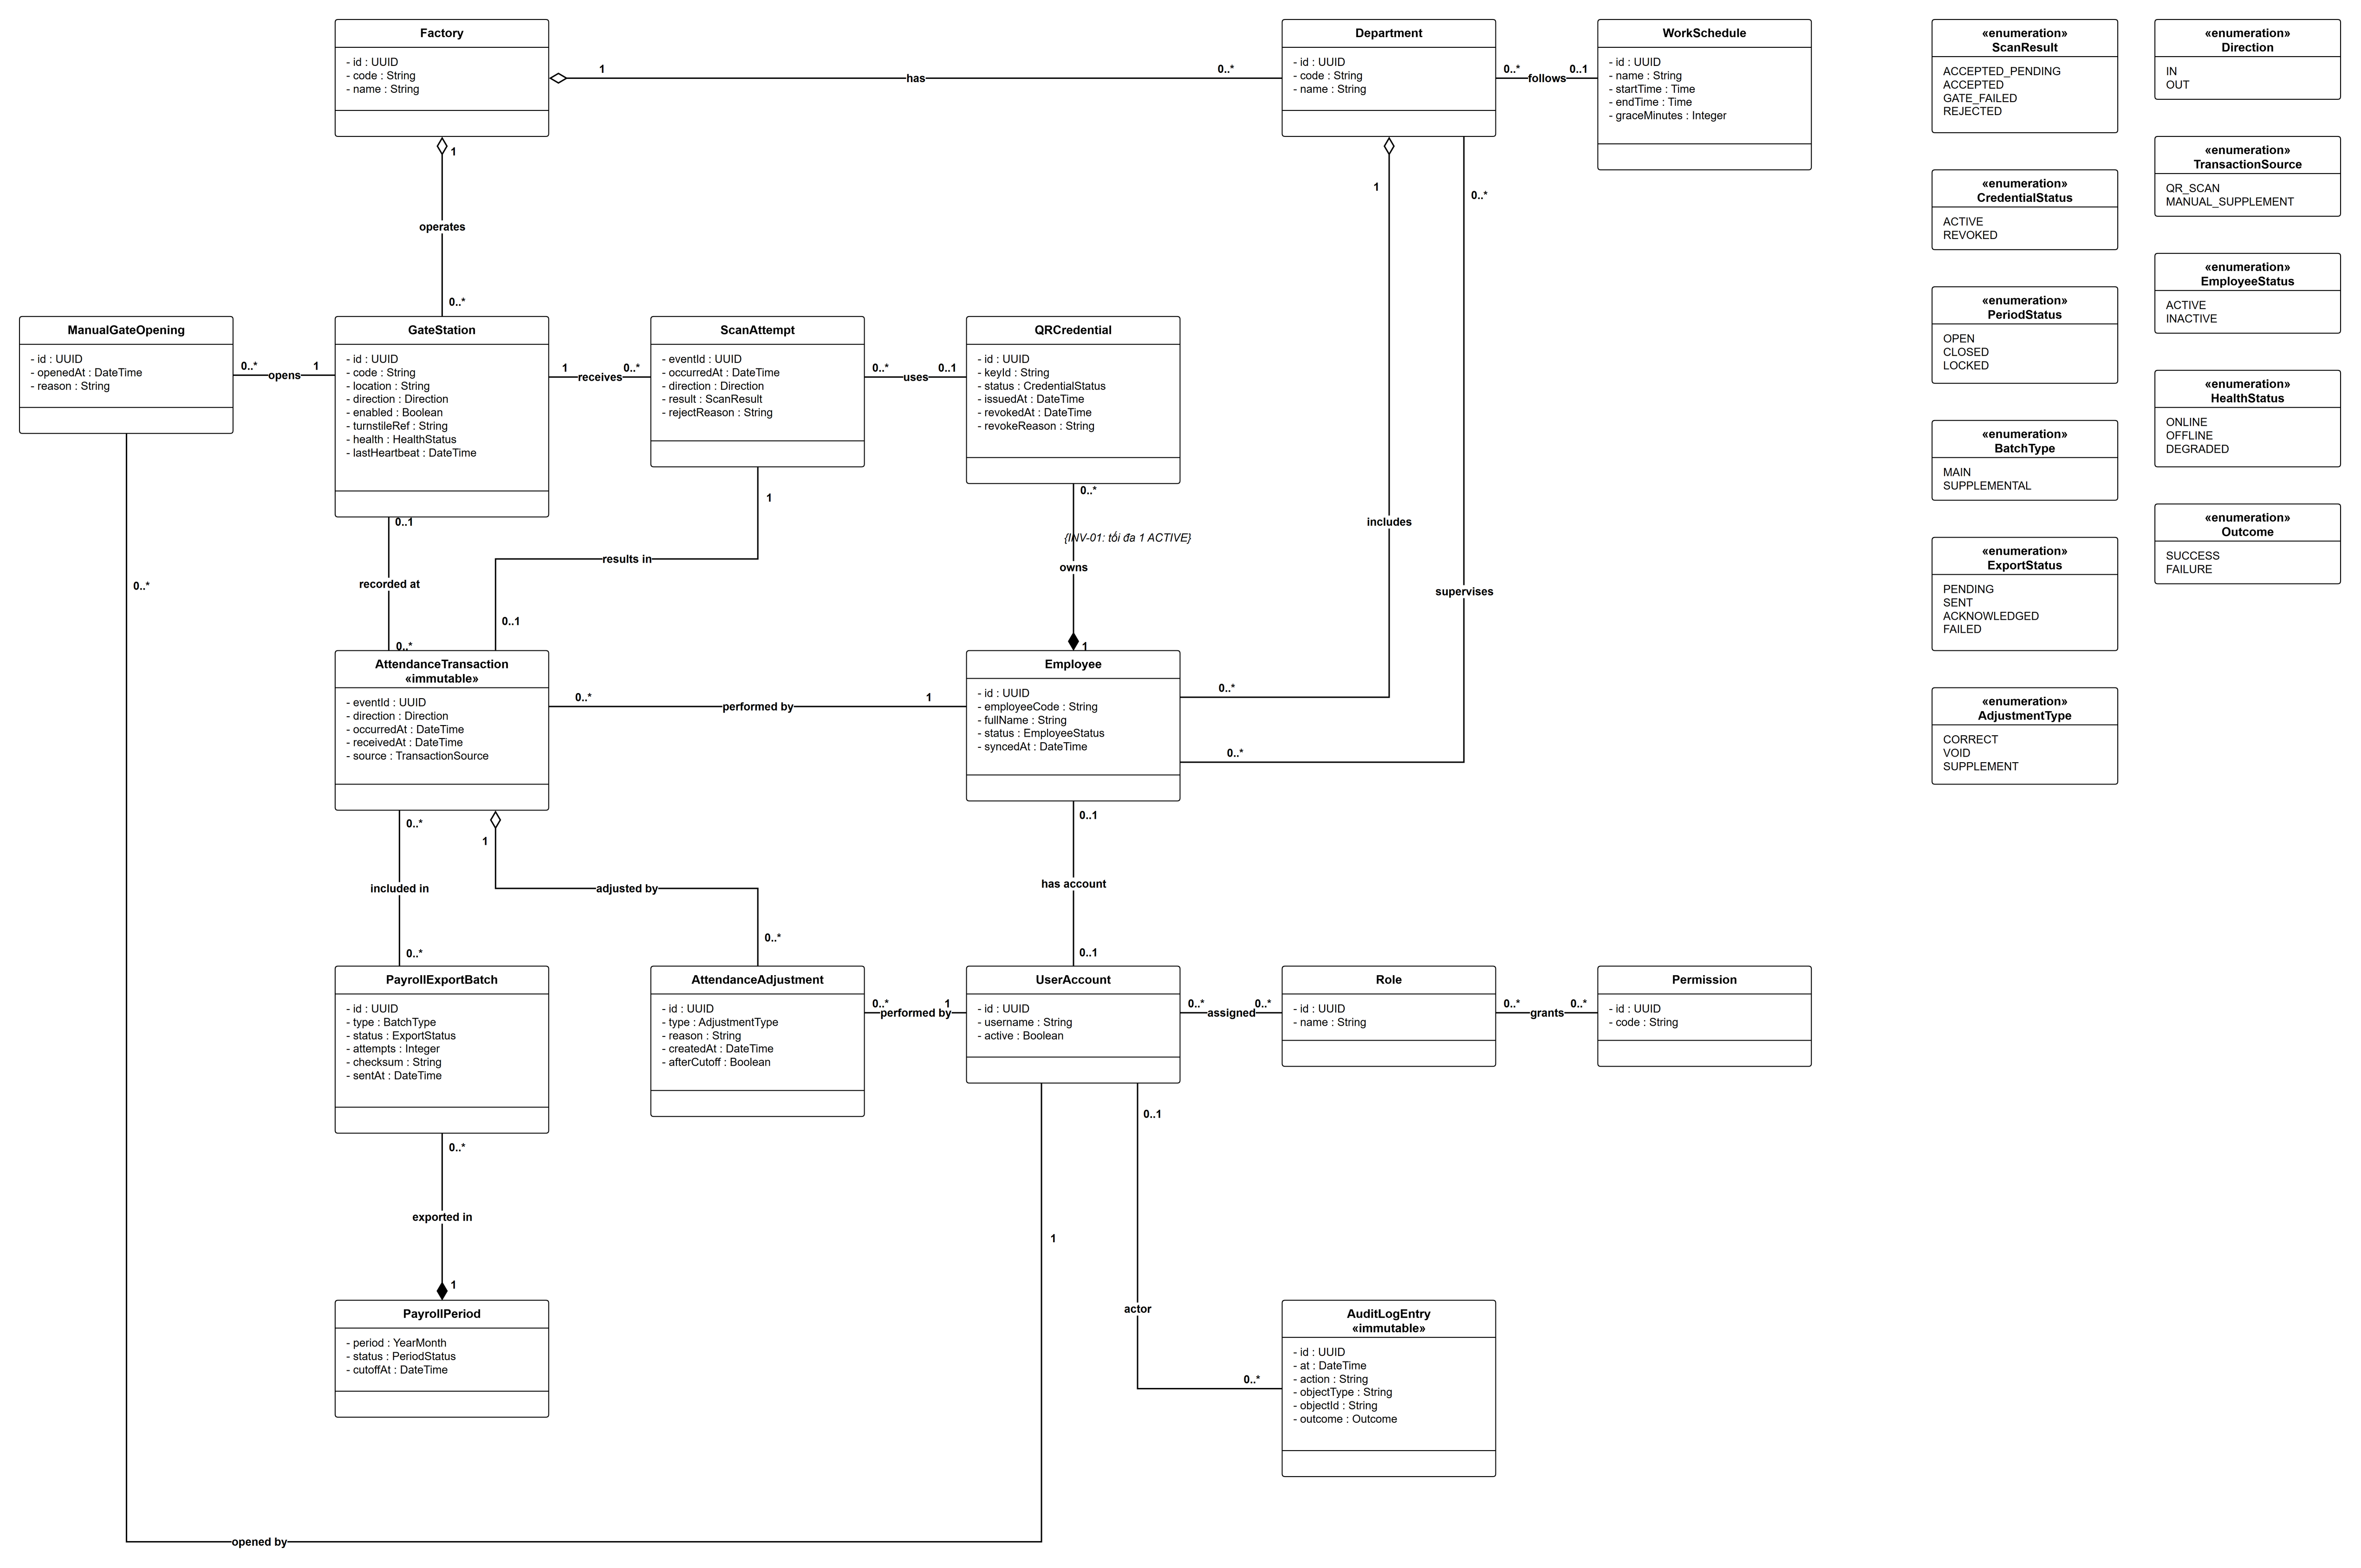
\includegraphics[width=0.92\textheight,height=0.92\textwidth,keepaspectratio]{figures/04_domain_model/class_diagram.png}}
    \caption{Lược đồ lớp mức nghiệp vụ của hệ thống chấm công và kiểm soát ra vào}
    \label{fig:sa-class-diagram}
\end{figure}

    \section{Đặc tính kiến trúc hệ thống}

Dựa trên bối cảnh nghiệp vụ, các yêu cầu chức năng, yêu cầu phi chức năng và những rủi ro đã xác định, hệ thống TMC có các đặc tính kiến trúc quan trọng sau đây.

\subsection{Architecture Characteristics Worksheet}

\small
\renewcommand{\arraystretch}{1.3}
\begin{longtable}{|>{\centering\arraybackslash}p{0.65cm}|>{\raggedright\arraybackslash}p{2.4cm}|>{\raggedright\arraybackslash}p{4.7cm}|>{\raggedright\arraybackslash}p{3.5cm}|>{\centering\arraybackslash}p{1.8cm}|}
\caption{Architecture Characteristics Worksheet} \\
\hline
\textbf{STT} & \textbf{Đặc tính kiến trúc} & \textbf{Mô tả trong bối cảnh hệ thống TMC} & \textbf{Cơ sở xác định} & \textbf{Mức độ ưu tiên} \\
\hline
\endfirsthead

\hline
\textbf{STT} & \textbf{Đặc tính kiến trúc} & \textbf{Mô tả trong bối cảnh hệ thống TMC} & \textbf{Cơ sở xác định} & \textbf{Mức độ ưu tiên} \\
\hline
\endhead

\hline
\endfoot

\hline
\endlastfoot

1 & Performance -- Hiệu năng & Đảm bảo quá trình xác thực QR, điều khiển cổng và phản hồi kết quả cho người dùng diễn ra nhanh chóng, đặc biệt trong giờ giao ca. & FR-14; NFR-AVL-02; R-01; mục 4.1 & Rất cao \\
\hline
2 & Availability -- Tính sẵn sàng & Duy trì hoạt động chấm công và kiểm soát ra vào khi xảy ra sự cố kết nối giữa trạm cổng và hệ thống trung tâm; hỗ trợ lưu trữ và đồng bộ dữ liệu khi kết nối được khôi phục. & FR-17; nhóm NFR-AVL; R-02 & Rất cao \\
\hline
3 & Reliability -- Độ tin cậy & Đảm bảo các giao dịch chấm công đã xác nhận được bảo toàn, việc gửi lại yêu cầu không tạo ra giao dịch trùng lặp và các lỗi tích hợp được xử lý phù hợp. & NFR-REL-01 đến NFR-REL-04; FR-21, FR-22; R-03, R-05 & Rất cao \\
\hline
4 & Data Integrity -- Tính toàn vẹn dữ liệu & Đảm bảo dữ liệu chấm công chính xác, đầy đủ và không bị ghi nhận trùng lặp; các điều chỉnh phải bảo toàn bản ghi gốc và lịch sử thay đổi. & NFR-DIN-01 đến NFR-DIN-04; FR-15, FR-16 & Rất cao \\
\hline
5 & Security -- Bảo mật & Ngăn chặn truy cập trái phép, kiểm soát quyền truy cập theo vai trò và chỉ cho phép mở cổng khi thông tin xác thực đáp ứng các điều kiện hợp lệ. & NFR-SEC-01 đến NFR-SEC-04; FR-25 đến FR-27 & Rất cao \\
\hline
6 & Interoperability -- Khả năng tương tác & Đảm bảo hệ thống trao đổi dữ liệu chính xác và nhất quán với hệ thống cổng xoay và hệ thống HR/Payroll thông qua các giao diện tích hợp được hỗ trợ. & NFR-INT-01 đến NFR-INT-04; C-01, C-02 & Cao \\
\hline
7 & Auditability -- Khả năng kiểm toán & Đảm bảo các thao tác quản trị, lần quét QR bị từ chối, sự kiện kiểm soát ra vào và các lần truyền dữ liệu đều được ghi nhận để phục vụ truy vết và kiểm tra khi cần thiết. & NFR-AUD-01 đến NFR-AUD-04; FR-23, FR-24 & Cao \\
\hline
8 & Privacy -- Bảo vệ dữ liệu cá nhân & Bảo vệ thông tin cá nhân của nhân viên thông qua kiểm soát quyền truy cập, giới hạn dữ liệu được chia sẻ cho các hệ thống liên quan và tuân thủ các quy định về bảo vệ dữ liệu cá nhân. & NFR-PRI-01 đến NFR-PRI-04; C-03 & Cao \\
\hline
9 & Recoverability -- Khả năng phục hồi & Đảm bảo dữ liệu chấm công có thể được khôi phục khi xảy ra sự cố, đồng thời duy trì các thông tin quan trọng cần thiết để xác định và đối chiếu giao dịch. & NFR-REC-01, NFR-REC-02 & Cao \\
\hline
10 & Scalability -- Khả năng mở rộng & Đảm bảo hệ thống có khả năng đáp ứng nhu cầu xử lý chấm công tại cả hai nhà máy và hỗ trợ sự gia tăng về số lượng nhân viên, trạm cổng và lưu lượng giao dịch. & Quy mô hệ thống tại mục 2.1; C-04; R-01 & Trung bình \\
\end{longtable}
\normalsize

\noindent\textbf{Nhận xét:} Các đặc tính có mức ưu tiên rất cao gồm hiệu năng, tính sẵn sàng, độ tin cậy, tính toàn vẹn dữ liệu và bảo mật. Đây là những yếu tố ảnh hưởng trực tiếp đến hoạt động kiểm soát ra vào, độ chính xác của dữ liệu chấm công và tính liên tục của nghiệp vụ tại hai nhà máy. Các đặc tính còn lại hỗ trợ việc tích hợp hệ thống, truy vết hoạt động, bảo vệ dữ liệu cá nhân, phục hồi sau sự cố và đáp ứng nhu cầu vận hành khi quy mô hệ thống tăng lên.

\subsection{Lựa chọn đặc tính kiến trúc ưu tiên (Top 3 Driving Factors)}

Dựa trên Architecture Characteristics Worksheet, ba đặc tính kiến trúc được lựa chọn làm yếu tố dẫn dắt chính cho hệ thống TMC là Performance, Reliability và Data Integrity. Việc lựa chọn này xuất phát từ yêu cầu xử lý nhanh các lượt quét QR, đảm bảo hoạt động chấm công đáng tin cậy và duy trì tính chính xác của dữ liệu phục vụ đối chiếu, tổng hợp và chuyển giao cho hệ thống HR/Payroll.

\small
\renewcommand{\arraystretch}{1.3}
\begin{longtable}{|>{\centering\arraybackslash}p{0.7cm}|>{\raggedright\arraybackslash}p{2.6cm}|>{\raggedright\arraybackslash}p{5.8cm}|>{\raggedright\arraybackslash}p{6.0cm}|}
\caption{Các đặc tính kiến trúc dẫn dắt chính} \\
\hline
\textbf{STT} & \textbf{Đặc tính kiến trúc} & \textbf{Cơ sở lựa chọn} & \textbf{Ảnh hưởng đến quyết định kiến trúc} \\
\hline
\endfirsthead
\hline
\textbf{STT} & \textbf{Đặc tính kiến trúc} & \textbf{Cơ sở lựa chọn} & \textbf{Ảnh hưởng đến quyết định kiến trúc} \\
\hline
\endhead
\hline
\endfoot
\hline
\endlastfoot
1 & Performance -- Hiệu năng & Hệ thống phải xử lý nhanh các lượt quét QR, đặc biệt trong giờ giao ca, nhằm hạn chế ùn tắc tại cổng. Báo cáo cũng xác định nguy cơ quá tải khi lưu lượng giao dịch tăng cao. & Ưu tiên luồng xử lý ngắn, hạn chế các thao tác đồng bộ không cần thiết trên luồng mở cổng và đảm bảo khả năng xử lý tải tại các trạm cổng. \\
\hline
2 & Reliability -- Độ tin cậy & Sự cố kết nối, lỗi điều khiển cổng hoặc lỗi tích hợp HR/Payroll có thể làm gián đoạn nghiệp vụ và ảnh hưởng đến việc chuyển giao dữ liệu đúng hạn. & Cần có cơ chế xử lý lỗi, thử lại có kiểm soát, theo dõi trạng thái giao dịch và đồng bộ dữ liệu sau khi kết nối được khôi phục. \\
\hline
3 & Data Integrity -- Tính toàn vẹn dữ liệu & Dữ liệu chấm công phải chính xác, không bị ghi nhận trùng lặp và có thể truy xuất lịch sử điều chỉnh. Sai lệch dữ liệu có thể ảnh hưởng đến quá trình đối chiếu ngày công và tính lương ở hệ thống bên ngoài. & Ưu tiên quản lý giao dịch nhất quán, định danh duy nhất cho các giao dịch, kiểm soát yêu cầu gửi lại và bảo toàn bản ghi gốc khi điều chỉnh. \\
\end{longtable}
\normalsize


Các đặc tính còn lại vẫn là những yêu cầu quan trọng của hệ thống, nhưng không được lựa chọn làm ba yếu tố dẫn dắt chính vì chúng có phạm vi tác động khác nhau hoặc có thể được xem xét như các yêu cầu cần đáp ứng trong quá trình hiện thực hóa kiến trúc.

\small
\renewcommand{\arraystretch}{1.3}
\begin{longtable}{|>{\raggedright\arraybackslash}p{4.2cm}|>{\raggedright\arraybackslash}p{10.7cm}|}
\caption{Lý do các đặc tính còn lại không thuộc Top 3 Driving Factors} \\
\hline
\textbf{Đặc tính kiến trúc} & \textbf{Lý do không thuộc Top 3 Driving Factors} \\
\hline
\endfirsthead
\hline
\textbf{Đặc tính kiến trúc} & \textbf{Lý do không thuộc Top 3 Driving Factors} \\
\hline
\endhead
\hline
\endfoot
\hline
\endlastfoot
Availability -- Tính sẵn sàng & Tính liên tục của hoạt động tại cổng rất quan trọng, đặc biệt khi mất kết nối. Tuy nhiên, trong phạm vi lựa chọn ba yếu tố dẫn dắt, vấn đề này được xem xét cùng với độ tin cậy và cơ chế xử lý lỗi, lưu trữ tạm thời, đồng bộ dữ liệu. Đặc tính này vẫn cần được đảm bảo trong thiết kế kiến trúc. \\
\hline
Security -- Bảo mật & Bảo mật là yêu cầu bắt buộc vì hệ thống xử lý thông tin nhân viên và kiểm soát quyền ra vào. Tuy nhiên, đây là yêu cầu nền tảng cần được áp dụng xuyên suốt các thành phần, thay vì được chọn làm yếu tố dẫn dắt chính cho cấu trúc xử lý nghiệp vụ trong phạm vi phân tích này. \\
\hline
Interoperability -- Khả năng tương tác & Việc tích hợp với cổng xoay và HR/Payroll là cần thiết, nhưng phạm vi tích hợp đã được xác định thông qua các giao diện và ràng buộc nghiệp vụ. Các vấn đề lỗi tích hợp, gửi lại dữ liệu và bảo toàn giao dịch được xem xét dưới góc độ Reliability và Data Integrity. \\
\hline
Auditability -- Khả năng kiểm toán & Ghi nhận nhật ký và truy vết là cần thiết cho quản trị và xử lý sự cố, nhưng không trực tiếp quyết định luồng xử lý giao dịch cốt lõi ở mức độ như ba đặc tính đã chọn. Yêu cầu này vẫn phải được đáp ứng thông qua cơ chế ghi nhật ký phù hợp. \\
\hline
Privacy -- Bảo vệ dữ liệu cá nhân & Việc bảo vệ dữ liệu cá nhân là nghĩa vụ cần tuân thủ. Các biện pháp liên quan đến phân quyền, giới hạn dữ liệu chia sẻ và quản lý lưu trữ cần được áp dụng xuyên suốt kiến trúc, nhưng không phải yếu tố dẫn dắt chính cho luồng giao dịch chấm công trong phân tích này. \\
\hline
Recoverability -- Khả năng phục hồi & Khả năng khôi phục dữ liệu sau sự cố rất quan trọng, nhưng chủ yếu liên quan đến sao lưu và phục hồi khi xảy ra sự cố. Trong phạm vi lựa chọn Top 3, đặc tính này được xem xét cùng các cơ chế bảo toàn dữ liệu và xử lý lỗi của Reliability và Data Integrity. \\
\hline
Scalability -- Khả năng mở rộng & Hệ thống hiện được xác định triển khai tại hai nhà máy với quy mô nhân sự đã nêu trong báo cáo. Yêu cầu nổi bật hiện tại là xử lý tải chấm công trong giờ giao ca; do chưa có mục tiêu tăng trưởng định lượng cụ thể, khả năng mở rộng chưa được chọn làm yếu tố dẫn dắt chính. \\
\end{longtable}
\normalsize

\subsection{Đánh giá sự đánh đổi (Trade-offs)}

Các đặc tính kiến trúc có thể hỗ trợ hoặc xung đột với nhau. Do đó, việc ưu tiên ba đặc tính trên cần đi kèm đánh giá những đánh đổi có thể phát sinh trong quá trình thiết kế và triển khai hệ thống TMC.

\small
\renewcommand{\arraystretch}{1.3}
\begin{longtable}{|>{\raggedright\arraybackslash}p{3.5cm}|>{\raggedright\arraybackslash}p{5.8cm}|>{\raggedright\arraybackslash}p{5.8cm}|}
\caption{Đánh giá trade-off giữa các đặc tính kiến trúc} \\
\hline
\textbf{Cặp đặc tính} & \textbf{Sự đánh đổi} & \textbf{Định hướng cân bằng} \\
\hline
\endfirsthead
\hline
\textbf{Cặp đặc tính} & \textbf{Sự đánh đổi} & \textbf{Định hướng cân bằng} \\
\hline
\endhead
\hline
\multicolumn{3}{r}{\textit{Còn tiếp sang trang sau...}} \\
\hline
\endfoot
\hline
\endlastfoot
Performance -- Reliability & Thử lại yêu cầu, chờ xác nhận từ hệ thống bên ngoài hoặc thực hiện các bước kiểm tra bổ sung có thể làm tăng thời gian xử lý một lượt quét. & Giới hạn thời gian chờ trên luồng xử lý tại cổng; tách việc xử lý lại và đồng bộ dữ liệu sang các tác vụ phù hợp khi không cần hoàn thành ngay để phản hồi người dùng. \\
\hline
Performance -- Data Integrity & Kiểm tra tính duy nhất, ghi nhận giao dịch bền vững và thực hiện các ràng buộc toàn vẹn có thể làm tăng độ trễ xử lý. & Tối ưu thao tác ghi dữ liệu và thiết kế giao dịch phù hợp, nhưng không bỏ qua các kiểm soát cần thiết để ngăn mất hoặc ghi nhận trùng dữ liệu chấm công. \\
\hline
Reliability -- Data Integrity & Cơ chế thử lại khi xảy ra lỗi có thể tạo giao dịch trùng lặp nếu hệ thống không xác định được yêu cầu đã được xử lý hay chưa. & Sử dụng định danh giao dịch ổn định, xử lý yêu cầu theo hướng idempotent và lưu trạng thái xử lý để việc thử lại không làm sai lệch dữ liệu. \\
\hline
Performance -- Security & Việc xác thực, kiểm tra quyền và kiểm tra trạng thái QR có thể làm tăng thời gian xử lý. & Tối ưu cơ chế xác thực và truy vấn trạng thái nhưng vẫn phải bảo đảm QR hợp lệ trước khi cho phép mở cổng. \\
\hline
Reliability -- Availability & Phụ thuộc hoàn toàn vào hệ thống trung tâm có thể khiến trạm cổng bị ảnh hưởng khi mạng gián đoạn; xử lý ngoại tuyến lại tạo thêm yêu cầu đồng bộ và kiểm soát tính nhất quán. & Xác định rõ phạm vi xử lý khi mất kết nối, chính sách lưu dữ liệu tạm thời và quy tắc đồng bộ sau khi hệ thống hoạt động trở lại. \\
\end{longtable}
\normalsize

Từ các đánh đổi trên, hệ thống cần ưu tiên thời gian phản hồi nhanh nhưng không đánh đổi tính chính xác và khả năng bảo toàn giao dịch. Đối với các thao tác không thể hoàn tất ngay do lỗi kết nối với hệ thống bên ngoài, cần phân biệt rõ trạng thái đã hoàn thành, đang chờ xử lý và thất bại thay vì thông báo thành công khi chưa có đủ căn cứ.

\noindent\textbf{Kết luận}

Performance, Reliability và Data Integrity là ba đặc tính kiến trúc dẫn dắt chính của hệ thống TMC. Các quyết định thiết kế cần cân bằng thời gian phản hồi nhanh với khả năng xử lý lỗi và bảo toàn tính chính xác của dữ liệu chấm công.
    \section{Cấu trúc kiến trúc hệ thống}

\subsection{Phân tích architecture quantum}
\subsubsection{Cơ sở phân tích}
Architecture quantum là đơn vị triển khai độc lập, có độ kết dính chức năng cao, ghép nối tĩnh chặt (cùng mã nguồn, cùng kho dữ liệu) và ghép nối động đồng bộ bên trong. Hai phần thuộc cùng một quantum khi phải triển khai cùng nhau, dùng chung kho dữ liệu hoặc gọi nhau đồng bộ trên đường xử lý chính (ví dụ quét QR và mở cổng tại trạm). Hai phần tách thành hai quantum khi cần bộ đặc tính kiến trúc khác nhau và liên lạc được bất đồng bộ (ví dụ xử lý tại cổng và báo cáo ở trung tâm). Cơ sở phân tích là bảng subdomain (mục 3.3) và các đặc tính ưu tiên (mục 4.2).

\subsubsection{So sánh đặc tính kiến trúc của thành phần xử lý tại trạm cổng và thành phần báo cáo}
Đặc tính kiến trúc chủ đạo (driving architecture characteristics) là những đặc tính phi chức năng có ảnh hưởng lớn nhất đến cấu trúc của một thành phần: thành phần không đạt mục tiêu nếu thiếu chúng, và để đạt được chúng phải lựa chọn cấu trúc, vị trí triển khai và công nghệ tương ứng. Bảng dưới so sánh hai thành phần nằm ở hai thái cực của hệ thống theo các tiêu chí này.

\begin{table}[H]
\centering
\caption{So sánh đặc tính kiến trúc của thành phần xử lý tại trạm cổng và thành phần báo cáo}
\small
\renewcommand{\arraystretch}{1.3}
\begin{tabularx}{\textwidth}{|>{\raggedright\arraybackslash}p{3.2cm}|>{\raggedright\arraybackslash}X|>{\raggedright\arraybackslash}X|}
\hline
\textbf{Tiêu chí so sánh} & \textbf{Xử lý tại trạm cổng (subdomain Kiểm soát ra vào)} & \textbf{Báo cáo và giám sát (subdomain Báo cáo)} \\
\hline
Đặc tính kiến trúc chủ đạo & Performance, Reliability và Availability (kèm khả năng vận hành khi mất kết nối) & Security và tính chính xác của dữ liệu tổng hợp \\
\hline
Yêu cầu về thời gian đáp ứng & Kết quả xử lý mỗi lần quét phải được trả về trong thời gian không quá 2 giây (NFR-01) & Chấp nhận độ trễ từ vài giây đến vài phút \\
\hline
Yêu cầu khi mất kết nối với trung tâm & Phải duy trì hoạt động độc lập, không làm gián đoạn việc ra vào (NFR-07) & Có thể tạm ngừng phục vụ mà không ảnh hưởng đến việc ra vào \\
\hline
Yêu cầu về toàn vẹn dữ liệu & Mỗi giao dịch phải được lưu bền vững trước khi xác nhận kết quả cho người dùng (NFR-02) & Dữ liệu chỉ đọc, được dẫn xuất từ các giao dịch đã ghi nhận \\
\hline
Đặc trưng truy cập dữ liệu & Ghi nhiều, chỉ thêm mới; đọc từ bản sao dữ liệu lưu cục bộ & Chỉ đọc; truy vấn tổng hợp theo tháng \\
\hline
Đặc điểm tải & Biến động mạnh, tập trung tại thời điểm đổi ca (ước tính 2 đến 5 giao dịch/giây mỗi nhà máy) & Tăng quanh kỳ chốt; số người dùng đồng thời thấp \\
\hline
Hệ quả khi xảy ra sự cố & Tắc nghẽn luồng người tại điểm kiểm soát; nguy cơ mất giao dịch & Chậm trễ trong việc khai thác báo cáo \\
\hline
Vị trí triển khai phù hợp & Tại từng nhà máy, gần cổng xoay & Tại trung tâm \\
\hline
\end{tabularx}
\end{table}

Hai thành phần chênh lệch ở cả đặc tính kiến trúc chủ đạo lẫn hệ quả khi xảy ra sự cố, nên không thể gộp vào cùng một quantum mà vẫn đáp ứng đồng thời NFR-01, NFR-02 và NFR-07.

\subsubsection{Bảng Subdomain, đặc tính cần và quantum}
Hệ thống gồm hai quantum: Q1 Gate Quantum đặt tại mỗi nhà máy và Q2 Central Quantum đặt tại trung tâm. Một số subdomain bị tách đôi vì hai nửa của chúng có đặc tính khác nhau.

\begin{table}[H]
\centering
\caption{Subdomain, đặc tính cần và quantum}
\small
\renewcommand{\arraystretch}{1.3}
\begin{tabularx}{\textwidth}{|>{\raggedright\arraybackslash}p{3.5cm}|>{\raggedright\arraybackslash}p{3.2cm}|>{\centering\arraybackslash}p{1.6cm}|>{\raggedright\arraybackslash}X|}
\hline
\textbf{Subdomain (mục 3)} & \textbf{Đặc tính cần (theo thứ tự)} & \textbf{Quantum} & \textbf{Ghi chú} \\
\hline
Kiểm soát ra vào: xác thực QR, mở cổng, ghi giao dịch (phía trạm cổng) & Performance, Reliability, Availability/Offline, Security & Q1 & Dùng bản sao cục bộ của danh sách QR hợp lệ và cấu hình trạm; lưu bền vững trước khi báo thành công \\
\hline
Tích hợp: adapter cổng xoay & Performance, Availability & Q1 & Gọi đồng bộ trong ngân sách 2 giây; có timeout và circuit breaker \\
\hline
Kiểm soát ra vào: nhận và lưu giao dịch (phía trung tâm) & Reliability/Data Integrity, Auditability & Q2 & Idempotent theo eventId \\
\hline
Điều chỉnh chấm công và chốt kỳ & Reliability/Data Integrity, Auditability, đúng hạn 12:00 ngày 1 & Q2 & Xử lý theo lô, chạy nền \\
\hline
Tích hợp: adapter HR/Payroll & Reliability (gửi lại khi lỗi), Interoperability & Q2 & Cách ly API bên ngoài khỏi nghiệp vụ lõi \\
\hline
Quản lý nhân viên và mã QR & Security, Privacy, Data Integrity & Q2 (nguồn dữ liệu), bản sao xuống Q1 & Độ trễ lan truyền thu hồi QR $\le$ 60 giây (đề xuất) \\
\hline
Quản lý trạm cổng & Availability (giám sát), Observability & Q2, bản sao cấu hình xuống Q1 & Heartbeat đi từ Q1 lên Q2 \\
\hline
Báo cáo và giám sát & Security (phạm vi dữ liệu), hiệu năng truy vấn mức vừa phải & Q2 & Module riêng, chỉ đọc \\
\hline
Xác thực, phân quyền và audit & Security, Auditability & Q2 & Thao tác mở cổng thủ công tại trạm cổng được ghi cục bộ rồi đồng bộ, để audit không bị mất \\
\hline
\end{tabularx}
\end{table}

\subsubsection{Tính độc lập về triển khai, mở rộng và chịu lỗi}

\begin{table}[H]
\centering
\caption{Tính độc lập về triển khai, mở rộng và chịu lỗi}
\small
\renewcommand{\arraystretch}{1.3}
\begin{tabularx}{\textwidth}{|>{\raggedright\arraybackslash}p{2.6cm}|>{\raggedright\arraybackslash}X|>{\raggedright\arraybackslash}X|>{\raggedright\arraybackslash}X|}
\hline
\textbf{Quantum} & \textbf{Triển khai} & \textbf{Mở rộng} & \textbf{Chịu lỗi} \\
\hline
Q1 Gate Quantum & Cập nhật theo từng nhà máy, không ảnh hưởng nhà máy còn lại & Theo số trạm cổng của nhà máy; thêm trạm chỉ là thêm cấu hình (NFR-08) & Trung tâm hỏng hoặc mất mạng thì cổng vẫn chạy; lỗi ở nhà máy này không lan sang nhà máy kia \\
\hline
Q2 Central Quantum & Theo kế hoạch bảo trì, không cần dừng cổng & Mở rộng dọc là đủ vì tải thấp (vài chục người dùng, vài giao dịch/giây) & Q2 hỏng thì báo cáo, điều chỉnh và đồng bộ tạm ngừng; giao dịch tích lại trong outbox tại Q1 và được gửi bù khi Q2 hoạt động lại \\
\hline
\end{tabularx}
\end{table}

Hai quantum ghép nối với nhau như sau:

Chiều xuống (Q2 sang Q1): danh sách QR hợp lệ và cấu hình trạm được nhân bản bất đồng bộ, nhất quán cuối cùng với độ trễ $\le$ 60 giây.

Chiều lên (Q1 sang Q2): giao dịch, lần quét bị từ chối, heartbeat và nhật ký mở cổng thủ công đi qua transactional outbox, chuyển giao ít nhất một lần và idempotent theo eventId.

Không có lời gọi đồng bộ từ Q1 lên Q2 trên đường xử lý lần quét. Đây là lý do đây là hai quantum riêng chứ không dính thành một.

Lời gọi đồng bộ còn lại (Q1 gọi cổng xoay) là lời gọi tới hệ thống ngoài tại cùng nhà máy; Q2 gọi HR/Payroll theo lô, bất đồng bộ.

\begin{table}[H]
\centering
\caption{So sánh phân rã theo kỹ thuật và phân rã theo domain}
\small
\renewcommand{\arraystretch}{1.3}
\begin{tabularx}{\textwidth}{|>{\raggedright\arraybackslash}p{3.8cm}|>{\raggedright\arraybackslash}X|>{\raggedright\arraybackslash}X|}
\hline
\diagbox[width=3.6cm]{\textbf{Tiêu chí}}{\textbf{Cách phân rã}} & \textbf{Phân rã theo kỹ thuật (technical partitioning)} & \textbf{Phân rã theo domain (domain partitioning)} \\
\hline
Nơi một thay đổi nghiệp vụ tác động (ví dụ thêm quy tắc anti-passback, thêm loại thiết bị xác thực) & Chạm nhiều tầng: giao diện, nghiệp vụ, dữ liệu & Gói trong một module của subdomain tương ứng \\
\hline
Phù hợp ranh giới nhất quán (mục 3.4) & Aggregate bị cắt ngang qua các tầng & Mỗi aggregate nằm trọn trong một module \\
\hline
Phù hợp quantum & Khó tách riêng phần chạy tại cổng & Tách tự nhiên theo vị trí triển khai \\
\hline
Làm việc song song trong nhóm & Dễ xung đột vì mọi tính năng đều đụng các tầng chung & Mỗi người phụ trách một module \\
\hline
\end{tabularx}
\end{table}

Kết luận: phân rã theo domain ở cấp cao nhất; mỗi module tương ứng một subdomain hoặc một nhóm subdomain nhỏ. Bên trong mỗi module dùng phân tầng hoặc ports and adapters để cách ly API bên ngoài (NFR-09).

\subsubsection{Kết luận về quantum}
Số quantum: hai loại, ba thể hiện triển khai (Gate Quantum tại Bình Dương và Long An, Central Quantum tại trung tâm).

Không tách thêm: báo cáo và chốt kỳ có đặc tính khác nhưng dùng chung kho dữ liệu trung tâm, tải thấp; chỉ giữ ranh giới module và quyền chỉ đọc.

Style phải hỗ trợ hai đơn vị triển khai độc lập, liên lạc bất đồng bộ, và đơn vị tại cổng chạy được khi mất kết nối.

\subsection{So sánh và lựa chọn architecture style}
\subsubsection*{Các Architecture Style được xem xét}
Sáu style ứng viên: layered, modular monolith, microkernel, service-based, event-driven và microservices. Mỗi style được đánh giá cho toàn hệ thống trong bối cảnh hai quantum ở mục 6.1.

\subsubsection*{Tiêu chí và trọng số}
Tiêu chí gồm ba đặc tính ưu tiên (mục 5.2), tiêu chí từ phân tích quantum (mục 6.1), ràng buộc dự án và một đặc tính thứ cấp. Trọng số từ 1 đến 3; thang điểm từ 1 đến 5 (5 là đáp ứng tốt nhất).

\begin{table}[H]
\centering
\caption{Tiêu chí và trọng số}
\small
\renewcommand{\arraystretch}{1.3}
\begin{tabularx}{\textwidth}{|>{\centering\arraybackslash}p{1cm}|>{\raggedright\arraybackslash}X|>{\raggedright\arraybackslash}p{4cm}|>{\centering\arraybackslash}p{1.8cm}|}
\hline
\textbf{Mã} & \textbf{Tiêu chí} & \textbf{Nguồn} & \textbf{Trọng số} \\
\hline
C1 & Reliability / Data Integrity & Đặc tính ưu tiên 1 & 3 \\
\hline
C2 & Performance & Đặc tính ưu tiên 2 & 3 \\
\hline
C3 & Security & Đặc tính ưu tiên 3 & 3 \\
\hline
C4 & Hỗ trợ hai quantum: Gate Quantum chạy độc lập và offline & Mục 6.1 & 3 \\
\hline
C5 & Chi phí và độ phức tạp vận hành & Ràng buộc & 2 \\
\hline
C6 & Năng lực nhóm và thời gian thực hiện & Ràng buộc & 2 \\
\hline
C7 & Modifiability / Interoperability (thêm thiết bị, thay đổi API ngoài) & Đặc tính thứ cấp, NFR-08, NFR-09 & 1 \\
\hline
\end{tabularx}
\end{table}

\subsubsection*{Bảng chấm điểm}
Điểm tổng bằng tổng của điểm từng tiêu chí nhân với trọng số, tối đa 85.

\begin{table}[H]
\centering
\caption{Chấm điểm}
\small
\renewcommand{\arraystretch}{1.3}
\begin{tabularx}{\textwidth}{|>{\raggedright\arraybackslash}X|*{7}{>{\centering\arraybackslash}p{0.75cm}|}>{\centering\arraybackslash}p{1.1cm}|}
\hline
\textbf{Style} & \textbf{C1} & \textbf{C2} & \textbf{C3} & \textbf{C4} & \textbf{C5} & \textbf{C6} & \textbf{C7} & \textbf{Tổng} \\
\hline
Layered & 2 & 3 & 3 & 1 & 5 & 5 & 2 & 49 \\
\hline
Modular monolith & 3 & 3 & 4 & 1 & 5 & 5 & 4 & 57 \\
\hline
Microkernel & 3 & 4 & 3 & 2 & 4 & 2 & 5 & 53 \\
\hline
Service-based (4 đến 6 dịch vụ) & 4 & 4 & 4 & 4 & 3 & 3 & 4 & 64 \\
\hline
Event-driven (có message broker) & 4 & 4 & 3 & 4 & 2 & 2 & 4 & 57 \\
\hline
Microservices & 3 & 3 & 3 & 5 & 1 & 1 & 5 & 51 \\
\hline
Hybrid đề xuất: modular monolith ở trung tâm, Gate Agent tại nhà máy, liên kết bằng outbox & 5 & 5 & 4 & 5 & 4 & 4 & 4 & 77 \\
\hline
\end{tabularx}
\end{table}

Điểm là đánh giá của nhóm trong bối cảnh TMC; cơ sở từng điểm được nêu trong bảng phân tích bên dưới.

\subsubsection*{Phân tích từng style trong bối cảnh TMC}

\begin{table}[H]
\centering
\caption{Phân tích từng style trong bối cảnh TMC}
\small
\renewcommand{\arraystretch}{1.3}
\begin{tabularx}{\textwidth}{|>{\raggedright\arraybackslash}p{2.3cm}|>{\raggedright\arraybackslash}X|>{\raggedright\arraybackslash}X|>{\raggedright\arraybackslash}p{2.2cm}|}
\hline
\textbf{Style} & \textbf{Ưu điểm trong bối cảnh TMC} & \textbf{Nhược điểm trong bối cảnh TMC} & \textbf{Kết luận} \\
\hline
Layered & Đơn giản, nhóm quen thuộc, chi phí thấp nhất & Phân rã kỹ thuật nên một thay đổi nghiệp vụ chạm nhiều tầng; xử lý tập trung ở trung tâm nên mất mạng thì cổng ngừng và có thể mất giao dịch (NFR-02, NFR-07) & Loại \\
\hline
Modular monolith & Ranh giới theo domain; giao dịch ACID giữ các invariant mạnh (INV-01, INV-09); chi phí thấp & Chỉ có một đơn vị triển khai nên xử lý tại cổng không chạy độc lập khi mất kết nối & Dùng cho phía trung tâm \\
\hline
Microkernel & Thêm thiết bị xác thực hoặc loại cổng xoay bằng plugin, khớp nguyên tắc Open/Closed và NFR-09 & Chốt kỳ và báo cáo không có tính plugin; tăng bề mặt tấn công; khung plugin tốn công với nhóm nhỏ & Dùng như kỹ thuật bên trong Gate Agent \\
\hline
Service-based (4 đến 6 dịch vụ) & Mỗi dịch vụ một domain; Gate là dịch vụ riêng; dùng chung CSDL nên giữ được ACID & Tách trung tâm thành nhiều tiến trình gọi nhau qua mạng, tăng chi phí vận hành khi tải thấp & Là nền tảng của hybrid, rút gọn còn hai dịch vụ \\
\hline
Event-driven (có broker) & Bất đồng bộ giữa Gate và Central, giữa Central và HR/Payroll; gửi lại khi lỗi & Phải vận hành broker, xử lý thứ tự và trùng lặp thông điệp với tải vài giao dịch/giây; thêm bề mặt bảo mật & Chỉ dùng outbox, không dùng broker \\
\hline
Microservices & Độc lập tối đa về triển khai và mở rộng & Chi phí vận hành cao so với 0,44 giao dịch/giây mỗi nhà máy; saga làm khó giữ toàn vẹn dữ liệu; nhóm nhỏ khó duy trì & Loại \\
\hline
\end{tabularx}
\end{table}

\subsubsection*{Kết luận về architecture style}
Style được chọn: hybrid gồm hai đơn vị triển khai. Central Quantum là modular monolith, mỗi module ứng với một subdomain. Gate Quantum là Gate Agent tại mỗi nhà máy, bên trong dùng ports and adapters và plugin kiểu microkernel cho thiết bị xác thực và adapter cổng xoay. Hai phía liên kết bất đồng bộ bằng transactional outbox, idempotent theo eventId, không dùng message broker. Về hình thức, đây là service-based với hai dịch vụ thô.

Lý do chọn:

Reliability: lưu bền vững cục bộ trước khi xác nhận; giao dịch ACID tại trung tâm.

Performance: đường xử lý lần quét chỉ dùng dữ liệu cục bộ.

Security: RBAC và audit tập trung ở trung tâm.

Hai quantum: Gate Agent chạy độc lập và offline; trung tâm bảo trì mà không dừng cổng.

Chi phí: chỉ hai đơn vị triển khai, không có broker.

Các đánh đổi kiến trúc:

Nhất quán cuối cùng: Dữ liệu giữa Gate Quantum và Central Quantum có thể tạm thời không đồng nhất. Việc thu hồi mã QR được phản ánh tại các trạm cổng với độ trễ tối đa 60 giây (INV-02, đề xuất).

Độ phức tạp tích hợp: Hệ thống phải duy trì cơ chế đồng bộ hai chiều, transactional outbox và cơ chế giám sát, gửi lại các giao dịch chưa được đồng bộ.

Phụ thuộc vào Central Quantum: Khi Central Quantum gặp sự cố, các chức năng báo cáo và đồng bộ với trung tâm tạm thời không hoạt động. Tuy nhiên, Gate Quantum vẫn tiếp tục thực hiện kiểm soát ra vào độc lập, nhờ đó sự cố tại trung tâm không làm gián đoạn hoạt động tại cổng.

\subsection{Kiến trúc logic}
Kiến trúc logic xác định các component của hệ thống TMC: mỗi component chịu trách nhiệm gì, đảm nhận FR nào, sở hữu dữ liệu gì và giao tiếp với nhau ra sao. Phần này chưa gắn với máy chủ hay công nghệ cụ thể; việc đặt component lên node thuộc kiến trúc vật lý (mục 6.4).

Component được xác định theo ba bước:

Đề xuất component ban đầu từ bảng subdomain (mục 3.3).

Gán các FR (mục 2.5) cho từng component.

Kiểm tra lại theo ba đặc tính ưu tiên (mục 5.2) và hai quantum (mục 6.1) để tách hoặc gộp.

\subsubsection{Xác định component}
Bước 1: Component ban đầu từ subdomain. Mỗi subdomain ở mục 3.3.2 cho một component ứng viên:

Kiểm soát ra vào và ghi nhận chấm công

Điều chỉnh chấm công và chốt kỳ

Quản lý nhân viên và mã QR

Quản lý trạm cổng

Báo cáo và giám sát

Tích hợp HR/Payroll và cổng xoay

Xác thực, phân quyền và audit

Bước 2: Gán FR. Khi gán FR-01 đến FR-26 cho bảy component ứng viên, nhóm thấy ba vấn đề:

"Kiểm soát ra vào" ôm FR của cả hai quantum. Các FR quyết định tại cổng (FR-10, FR-11, FR-13) cần chạy ở Q1. Còn việc lưu trữ giao dịch phục vụ báo cáo và chốt kỳ (FR-12, FR-14) thuộc Q2.

"Tích hợp" gộp hai hệ thống ngoài có cách gọi trái ngược. Cổng xoay được gọi đồng bộ ở mỗi lần quét, trong ngân sách 2 giây. HR/Payroll được gọi theo lô vào cuối tháng.

FR-09 và một phần FR-08 cần chạy được ngay tại cổng khi mất kết nối. FR-09 là mở cổng thủ công; phần FR-08 liên quan là hiển thị trạng thái trạm. Trong khi đó component "Quản lý trạm cổng" lại nằm ở trung tâm.

Bước 3: Kiểm tra theo đặc tính ưu tiên và quantum. Từ ba vấn đề trên, nhóm tách và gộp như sau:

Tách "Kiểm soát ra vào" theo quantum (mục 6.1.3).

Access Control (G1) đặt tại cổng, phục vụ Performance và Availability/Offline.

Gate Sync \& Ingestion (C1) đặt ở trung tâm, phục vụ Reliability/Data Integrity.

Tách "Tích hợp" thành hai adapter: Turnstile Adapter (G2, thuộc Q1) và HR/Payroll Adapter (C5, thuộc Q2), vì hai phía khác nhau cả về đặc tính lẫn quantum.

Thêm hai component kỹ thuật: Local Store \& Outbox (G3) và Gate Sync Agent (G4). Hai component này không có FR riêng, nhưng bắt buộc phải có để Q1 lưu bền vững trước khi xác nhận (INV-05) và đồng bộ được với Q2 (mục 6.1.4).

Thêm Guard Console (G5) tại cổng cho FR-09 và cho việc hiển thị lần quét bị từ chối, để bảo vệ vẫn thao tác được khi mất mạng.

Tách "Xác thực, phân quyền và audit" thành IAM/RBAC (C7) và Audit Log (C8). Audit Log chỉ ghi thêm và có quy tắc truy cập, thời hạn lưu riêng (NFR-05, INV-10). Nó còn nhận cả bản ghi mở cổng thủ công đồng bộ lên từ Q1.

Tách Configuration (C9) khỏi Quản lý trạm cổng, vì tham số hệ thống (FR-26) được nhiều module dùng chung.

Giữ "Điều chỉnh chấm công và chốt kỳ" thành một component (C4). Điều chỉnh và chốt kỳ cùng chịu INV-09: sau khi khóa kỳ, điều chỉnh phải đi vào đợt bổ sung. Nếu tách hai nơi thì phải đồng bộ trạng thái kỳ giữa chúng.

Không tách Báo cáo (C6) thành quantum riêng (mục 6.1.5). C6 chỉ đọc qua read model.

Kết quả là 14 component, trình bày trong Bảng 6.3.1. Mọi FR từ FR-01 đến FR-26 đều có component đảm nhận. Các FR trải trên cả hai quantum (FR-08, FR-11, FR-12, FR-14) được chia thành phần phía cổng và phần phía trung tâm.

\small
\renewcommand{\arraystretch}{1.3}
\begin{longtable}{|>{\centering\arraybackslash}p{0.8cm}|>{\raggedright\arraybackslash}p{2.5cm}|>{\raggedright\arraybackslash}p{6.0cm}|>{\raggedright\arraybackslash}p{2.2cm}|>{\raggedright\arraybackslash}p{2.8cm}|}
% --- Tiêu đề duy nhất ở trang đầu ---
\caption{Danh mục component} \label{tab:danh_muc_component} \\
\hline
\textbf{Mã} & \textbf{Component} & \textbf{Trách nhiệm} & \textbf{FR đảm nhận} & \textbf{Đặc tính phải đáp ứng} \\
\hline
\endfirsthead

% --- Sang trang sau: chỉ kẻ lại tiêu đề cột (không in tiêu đề bảng) ---
\hline
\textbf{Mã} & \textbf{Component} & \textbf{Trách nhiệm} & \textbf{FR đảm nhận} & \textbf{Đặc tính phải đáp ứng} \\
\hline
\endhead

\endfoot

\hline
\endlastfoot

\multicolumn{5}{|l|}{\textbf{Q1 Gate Quantum: Gate Agent, mỗi nhà máy một bản}} \\
\hline
G1 & Access Control & Xác thực QR bằng danh sách QR hợp lệ cục bộ (QR ở trạng thái ACTIVE, nhân viên đang hoạt động); kiểm tra trạm đang bật (INV-03) và anti-passback (INV-04); quyết định cho qua; ghi giao dịch hoặc lần quét bị từ chối; hiển thị kết quả trên kiosk & FR-10, FR-11, FR-12, FR-13, FR-14 & Performance, Reliability/Data Integrity, Availability/Offline, Security \\
\hline
G2 & Turnstile Adapter & Gọi API cổng xoay, có timeout và circuit breaker; mỗi nhà cung cấp là một plugin & FR-11 & Performance, Availability, Interoperability \\
\hline
G3 & Local Store \& Outbox & Kho cục bộ bền vững, có mã hóa. Giữ bản sao danh sách QR hợp lệ và cấu hình trạm; giữ AttendanceTransaction, ScanAttempt và ManualGateOpening chờ đồng bộ (outbox) & FR-12, FR-14 & Reliability/Data Integrity, Privacy \\
\hline
G4 & Gate Sync Agent & Đẩy outbox lên trung tâm (giao ít nhất một lần); kéo danh sách QR hợp lệ và cấu hình trạm về (trễ $\le$ 60 giây); gửi heartbeat & FR-08 & Reliability/Data Integrity, Availability/Offline \\
\hline
G5 & Guard Console & Hiển thị lần quét bị từ chối và trạng thái trạm ngay tại chỗ; mở cổng thủ công, bắt buộc nhập lý do và ghi vào G3 để đồng bộ audit & FR-09, FR-10, FR-15 & Availability/Offline, Security, Auditability \\
\hline
\multicolumn{5}{|l|}{\textbf{Q2 Central Quantum: modular monolith}} \\
\hline
C1 & Gate Sync \& Ingestion & Nhận dữ liệu từ các Gate Agent, idempotent theo eventId (INV-06); lưu giao dịch bất biến; cung cấp danh sách QR hợp lệ và cấu hình cho Gate Agent & FR-12, FR-14 & Reliability/Data Integrity, Security \\
\hline
C2 & Employee \& QR Management & Quản lý hồ sơ nhân viên; cấp, thu hồi và cấp lại QR (INV-01); hiển thị QR qua app, web portal, email & FR-01 – FR-04 & Security, Privacy, Reliability/Data Integrity \\
\hline
C3 & Gate Station Management & Đăng ký, cập nhật, bật/tắt trạm; theo dõi trạng thái qua heartbeat và cảnh báo khi trạm offline & FR-06 – FR-08 & Availability, Observability, Scalability \\
\hline
C4 & Adjustment \& Period Closing & Điều chỉnh giao dịch có lý do, giữ bản gốc (INV-08); quản lý kỳ qua các trạng thái OPEN $\rightarrow$ CLOSED $\rightarrow$ LOCKED và các đợt MAIN, SUPPLEMENTAL (INV-09); theo dõi trạng thái truyền dữ liệu & FR-16, FR-21, FR-22 & Reliability/Data Integrity, Auditability \\
\hline
C5 & HR/Payroll Adapter & Gửi đợt dữ liệu sang HR/Payroll; gửi lại khi lỗi; idempotent theo mã đợt & FR-19, FR-20 & Reliability/Data Integrity, Interoperability \\
\hline
C6 & Reporting \& Monitoring & Read model chỉ đọc cho báo cáo tháng, lịch sử chấm công cá nhân và màn hình theo dõi; lọc dữ liệu theo phạm vi của người xem (INV-11) & FR-05, FR-18 – FR-20 & Security, Privacy \\
\hline
C7 & IAM / RBAC & Đăng nhập; quản lý tài khoản, vai trò, quyền; kiểm tra quyền cho mọi API & FR-25, FR-26, FR-27 & Security \\
\hline
C8 & Audit Log & Ghi nhật ký chỉ thêm cho các thao tác quan trọng, kể cả thao tác từ Q1; tra cứu, lọc; lưu tối thiểu 12 tháng (INV-10) & FR-23, FR-24 & Auditability, Security, Privacy \\
\hline
C9 & Configuration & Tham số hệ thống: lịch truyền dữ liệu HR, thời gian lưu dữ liệu, ngưỡng mất kết nối của cổng & FR-28 & Modifiability, Scalability \\
\end{longtable}
\normalsize

\subsubsection{Sơ đồ component và cách giao tiếp}
Hình 6.3.1 là sơ đồ component; Bảng 6.3.2 ghi kiểu giao tiếp và interface giữa từng cặp component. Hệ thống có ba luồng với đặc tính khác nhau:

Luồng quét (đồng bộ, $\le$ 2 giây, chỉ trong Q1): máy quét $\rightarrow$ G1 $\rightarrow$ G3 $\rightarrow$ G2 $\rightarrow$ cổng xoay.

Luồng đồng bộ (bất đồng bộ, gần thời gian thực): G3 $\rightarrow$ G4 $\rightarrow$ C1 khi đi lên, và C1 $\rightarrow$ G4 $\rightarrow$ G3 khi đi xuống.

Luồng chốt kỳ (theo lô): C4 $\rightarrow$ C5 $\rightarrow$ HR/Payroll.

\begin{figure}[H]
\centering
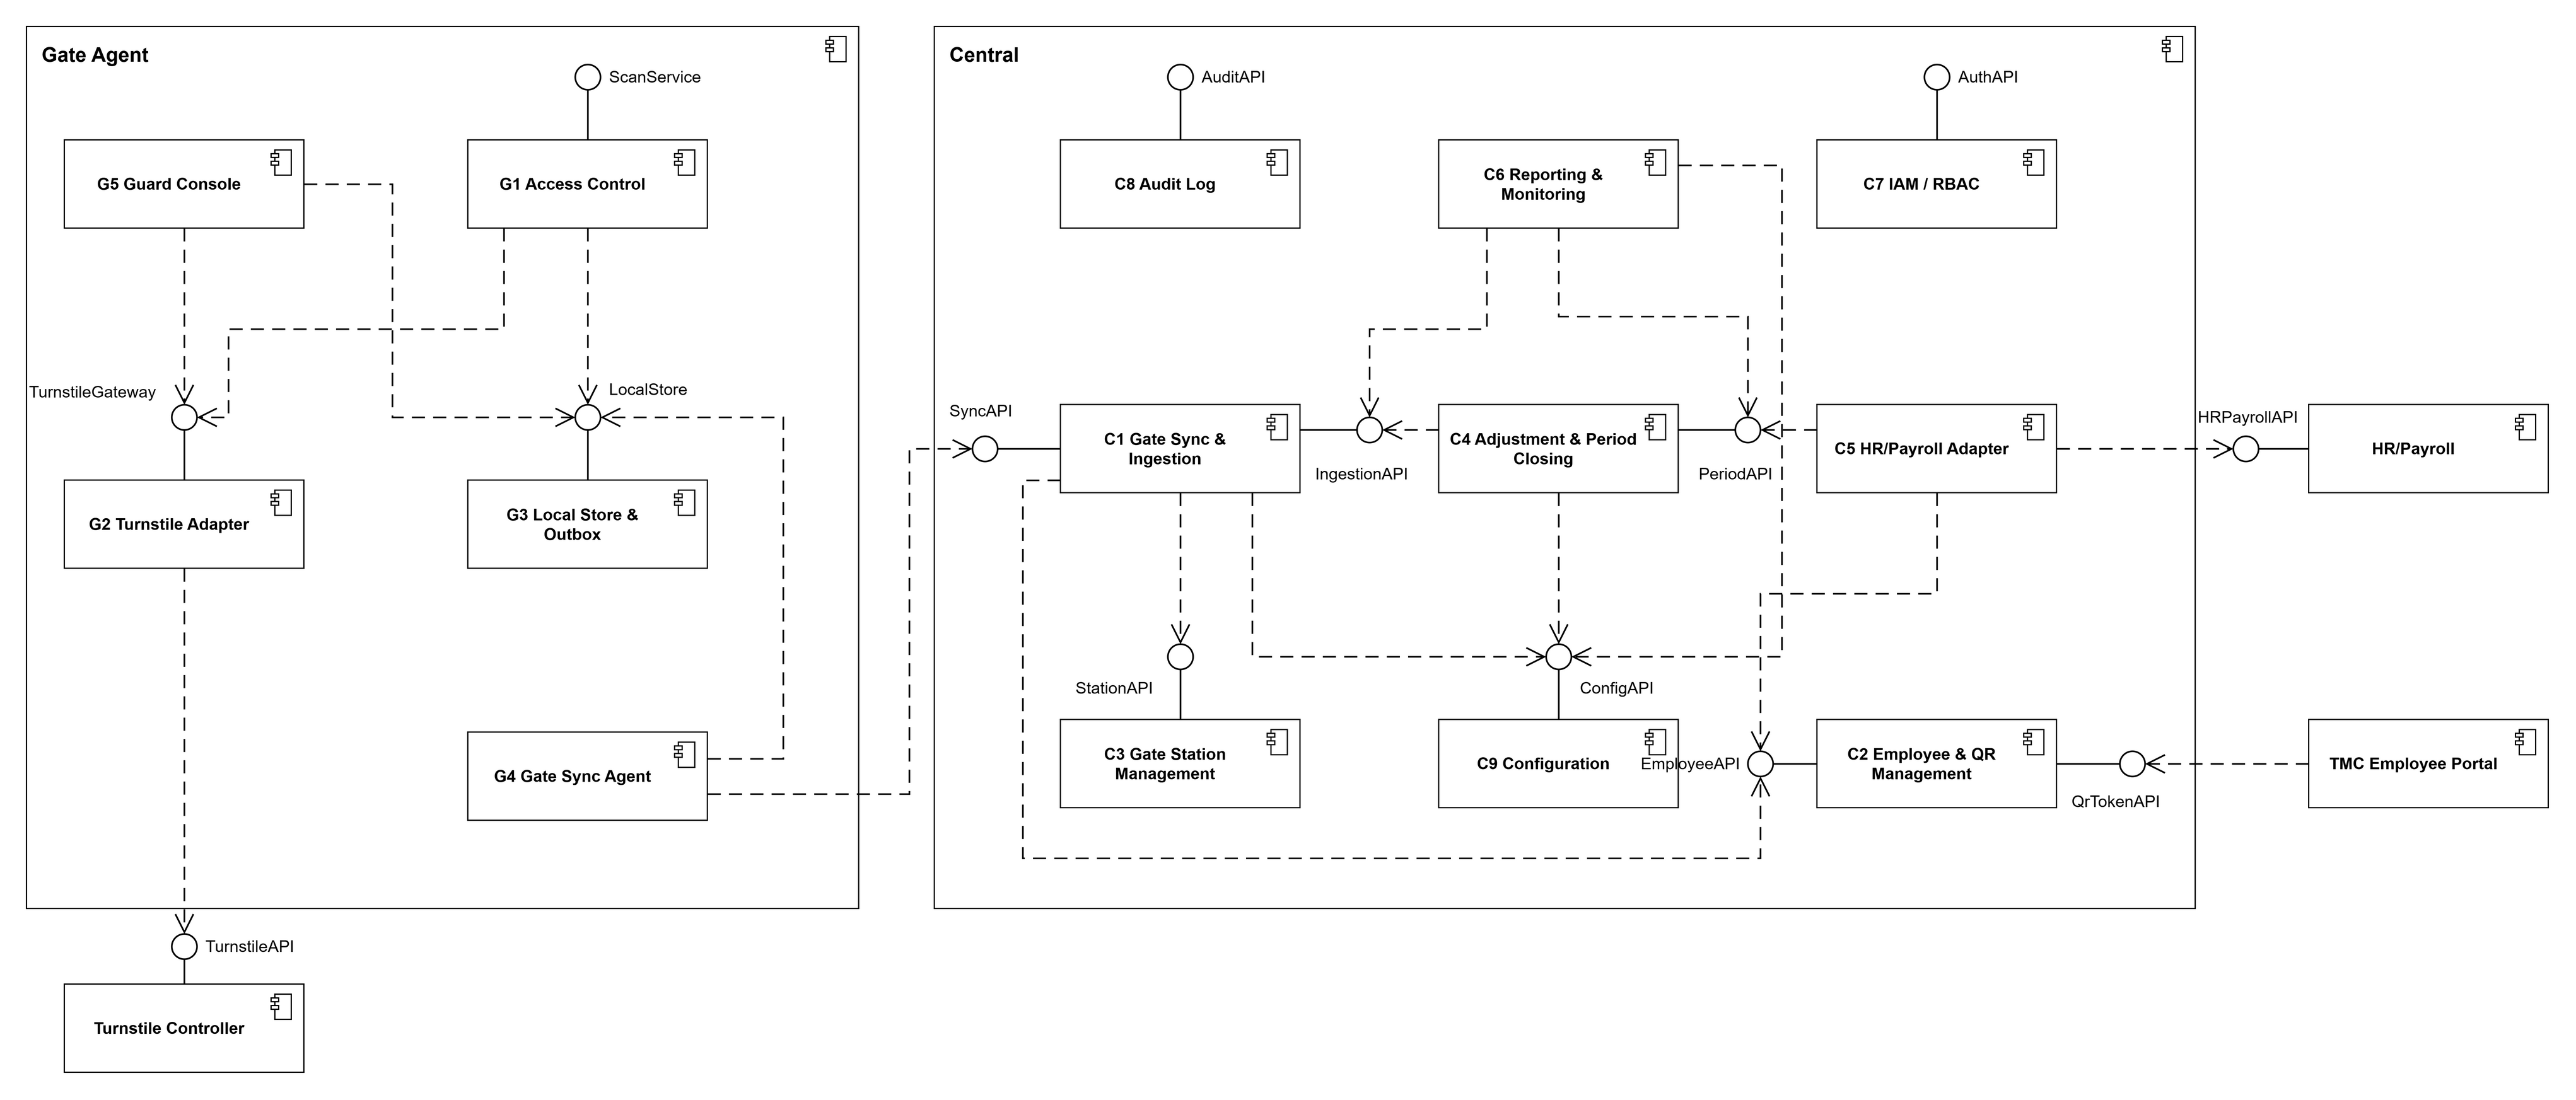
\includegraphics[width=0.9\textwidth]{figures/06_architecture_structure/component_diagram.png}
\caption{Sơ đồ component của hệ thống TMC.}
\label{fig:component_diagram}
\end{figure}

Mũi tên liền là lời gọi đồng bộ; mũi tên đứt là truyền bất đồng bộ.

G5 gọi G2 khi bảo vệ mở cổng thủ công.

Mọi module trung tâm đều ghi vào Audit Log (C8).

C1 lấy danh sách QR hợp lệ từ C2 và lấy cấu hình từ C3, C9 để cấp cho Gate Agent.

\begin{table}[H]
\centering
\small
\renewcommand{\arraystretch}{1.3}
\caption{Cách giao tiếp giữa các component}
\begin{tabularx}{\textwidth}{|>{\raggedright\arraybackslash}p{3.2cm}|>{\raggedright\arraybackslash}p{3.2cm}|>{\raggedright\arraybackslash}X|}
\hline
\textbf{Từ $\rightarrow$ Đến} & \textbf{Kiểu giao tiếp} & \textbf{Interface / nội dung} \\
\hline
Máy quét $\rightarrow$ G1 & Đồng bộ, cục bộ & Sự kiện quét (nội dung QR, mã trạm) \\
\hline
G1 $\rightarrow$ G3 & Đồng bộ, cục bộ & AllowlistReader.find(), TransactionStore.append() \\
\hline
G1, G5 $\rightarrow$ G2 & Đồng bộ, có timeout & TurnstileGateway.open() \\
\hline
G2 $\rightarrow$ Hệ thống cổng xoay & Đồng bộ, mạng nội bộ nhà máy & API cổng xoay (C-01) \\
\hline
G5 $\rightarrow$ G3 & Đồng bộ, cục bộ & Ghi ManualGateOpening \\
\hline
G3 $\rightarrow$ G4 $\rightarrow$ C1 & Bất đồng bộ, giao ít nhất một lần, idempotent theo eventId & Giao dịch, lần quét bị từ chối, mở cổng thủ công, heartbeat \\
\hline
C1 $\rightarrow$ G4 $\rightarrow$ G3 & Bất đồng bộ, kéo định kỳ, trễ $\le$ 60 giây & Danh sách QR hợp lệ, cấu hình trạm \\
\hline
C2, C3, C9 $\rightarrow$ C1 & Domain event trong tiến trình & QrCredentialChanged, StationConfigChanged, SettingChanged \\
\hline
C1 $\rightarrow$ C4, C6 & Domain event trong tiến trình & TransactionRecorded \\
\hline
C4 $\rightarrow$ C6 & Domain event trong tiến trình & AdjustmentRecorded, PeriodStatusChanged \\
\hline
C4 $\rightarrow$ C5 & Bất đồng bộ qua outbox trung tâm & ExportBatchReady \\
\hline
C5 $\rightarrow$ HR/Payroll & Bất đồng bộ theo lô, gửi lại khi lỗi & HrPayrollGateway.submit() (C-01) \\
\hline
Client $\rightarrow$ C7 $\rightarrow$ các module & Đồng bộ, HTTPS & API của từng module; kiểm tra quyền trước khi xử lý \\
\hline
Mọi module $\rightarrow$ C8 & Trong tiến trình, ghi bền vững & AuditLog.record() \\
\hline
\end{tabularx}
\end{table}

F1 – Quét QR qua cổng.

G1 nhận nội dung QR từ máy quét và tra trong danh sách QR hợp lệ ở G3. G1 kiểm tra:

QR ở trạng thái ACTIVE và nhân viên đang hoạt động;

trạm đang bật (INV-03);

lần quét không vi phạm anti-passback (INV-04).

Nếu hợp lệ: G1 ghi AttendanceTransaction kèm eventId vào G3 trước. Chỉ sau đó G1 mới gửi lệnh mở cổng qua G2 và báo thành công trên kiosk (INV-05). Nếu không hợp lệ: G1 ghi ScanAttempt kèm lý do (INV-07) và hiển thị kết quả trên cả kiosk lẫn G5.

Nếu gọi cổng xoay lỗi hoặc quá thời gian: giao dịch đã ghi vẫn giữ nguyên, và bảo vệ xử lý tại G5 bằng cách mở cổng thủ công (FR-09). Nếu nhân viên cuối cùng không qua cổng, HR hủy giao dịch bằng điều chỉnh (FR-15).

Toàn bộ luồng chỉ dùng dữ liệu cục bộ. Phần lớn ngân sách 2 giây dành cho cổng xoay, vốn mất tối đa 500 ms (A-03).

F2 – Đồng bộ giữa hai quantum.

Chiều lên: G4 đọc outbox trong G3 và gửi lên C1. C1 bỏ qua bản trùng theo eventId rồi gửi xác nhận. G4 chỉ đánh dấu một bản ghi là đã gửi khi nhận được xác nhận.

Chiều xuống: G4 kéo danh sách QR hợp lệ và cấu hình trạm về. Khi có mạng, độ trễ không quá 60 giây (INV-02).

Heartbeat: G4 gửi heartbeat định kỳ để C3 phát hiện trạm offline.

F3 – Điều chỉnh và chốt kỳ.

Điều chỉnh: HR điều chỉnh giao dịch qua C4, bắt buộc có lý do. Giao dịch gốc được giữ nguyên (INV-08) và mọi thao tác được ghi vào C8.

Chốt kỳ: đến lịch đặt trong C9, C4 chuyển kỳ sang CLOSED, tạo đợt MAIN và đưa vào outbox trung tâm. C5 gửi đợt này sang HR/Payroll; nếu lỗi thì gửi lại chính đợt đó. Lịch chốt được đặt đủ sớm để còn thời gian dự phòng trước 12:00 ngày 1 (NFR-03). C4 phát cảnh báo nếu đến sát hạn mà đợt MAIN vẫn chưa được HR/Payroll xác nhận.

Sau khi khóa kỳ: khi kỳ đã ở trạng thái LOCKED, mọi điều chỉnh mới đi vào đợt SUPPLEMENTAL (INV-09).

F4 – Gate Agent mất kết nối. Gate Agent vận hành theo Bảng 6.3.3.

\begin{table}[H]
\centering
\small
\renewcommand{\arraystretch}{1.3}
\caption{Hành vi của Gate Agent theo trạng thái kết nối}
\begin{tabularx}{\textwidth}{|>{\raggedright\arraybackslash}p{3.5cm}|>{\raggedright\arraybackslash}X|>{\raggedright\arraybackslash}X|}
\hline
\textbf{Trạng thái} & \textbf{Chiều vào} & \textbf{Chiều ra} \\
\hline
Có kết nối & Bình thường; danh sách QR hợp lệ cập nhật với độ trễ $\le$ 60 giây & Bình thường \\
\hline
Mất kết nối, chưa quá ngưỡng (ngưỡng đặt ở C9) & Vẫn hoạt động bằng dữ liệu cục bộ; dữ liệu tích lại trong outbox; C3 cảnh báo khi mất heartbeat & Bình thường \\
\hline
Mất kết nối, quá ngưỡng & Fail-closed: cổng không tự mở; bảo vệ mở thủ công qua G5 (FR-09, bắt buộc lý do, có audit) & Luôn cho ra vì an toàn cháy nổ; lần quét vẫn được ghi để chấm công \\
\hline
\end{tabularx}
\end{table}

Giá trị ngưỡng mất kết nối sẽ được chốt cùng giảng viên, như đã nêu ở mục 5.2. Khi có mạng trở lại, luồng F2 gửi bù toàn bộ outbox; eventId bảo đảm không tạo bản ghi trùng.

\subsection{Kiến trúc vật lý}
Kiến trúc vật lý xác định cách thức các thành phần Component được ánh xạ và triển khai trên Nodes, môi trường thực thi, cấu hình mạng và đường truyền vật lý, nhằm hiện thực hóa các mục tiêu về hiệu năng, độ tin cậy không mất mát dữ liệu và tính sẵn sàng/ khả năng tự vận hành offline.

\subsubsection{Lựa chọn Topology triển khai}
Hệ thống TMC được quyết định triển khai theo mô hình Hybrid Edge-Central Topology (Kết hợp điện toán biên tại nhà máy và điện toán tập trung tại máy chủ trung tâm):  

Phần xử lý tại từng nhà máy (Edge - Gate Quantum Q1):
\begin{itemize}
    \item Toàn bộ phần mềm quét mã, xác thực và điều khiển mở cổng được cài đặt trực tiếp trên máy tính tại trạm cổng (Kiosk) của 2 nhà máy (Bình Dương và Long An).
    \item Mục đích: Xử lý ngay tại mạng nội bộ để đảm bảo tốc độ phản hồi cực nhanh ($\le$ 2 giây - NFR-01), giải quyết triệt để bài toán ùn tắc giờ cao điểm đổi ca, đồng thời giúp cổng vẫn tự hoạt động bình thường kể cả khi mất kết nối Internet về trung tâm (NFR-07, NFR-10).
\end{itemize}

Phần xử lý tập trung (Central - Central Quantum Q2):
\begin{itemize}
    \item Toàn bộ phần mềm quản lý nhân sự, phân quyền người dùng (RBAC), lưu trữ dữ liệu tổng và đối soát lương được đặt tập trung trên máy chủ trung tâm (Cloud / Datacenter).
    \item Mục đích: Đảm bảo an toàn, nhất quán dữ liệu và kiểm toán tập trung (NFR-02, NFR-04, NFR-05), phục vụ việc tổng hợp báo cáo và truyền dữ liệu sang hệ thống HR/Payroll đúng hạn chốt lương hằng tháng (C-02, NFR-03).
\end{itemize}

\subsubsection{Sơ đồ triển khai vật lý}
Sơ đồ triển khai dưới đây mô tả cấu trúc vật lý, vị trí của từng thành phần, ranh giới mạng và phương thức liên kết giữa các hệ thống:

\begin{figure}[H]
\centering
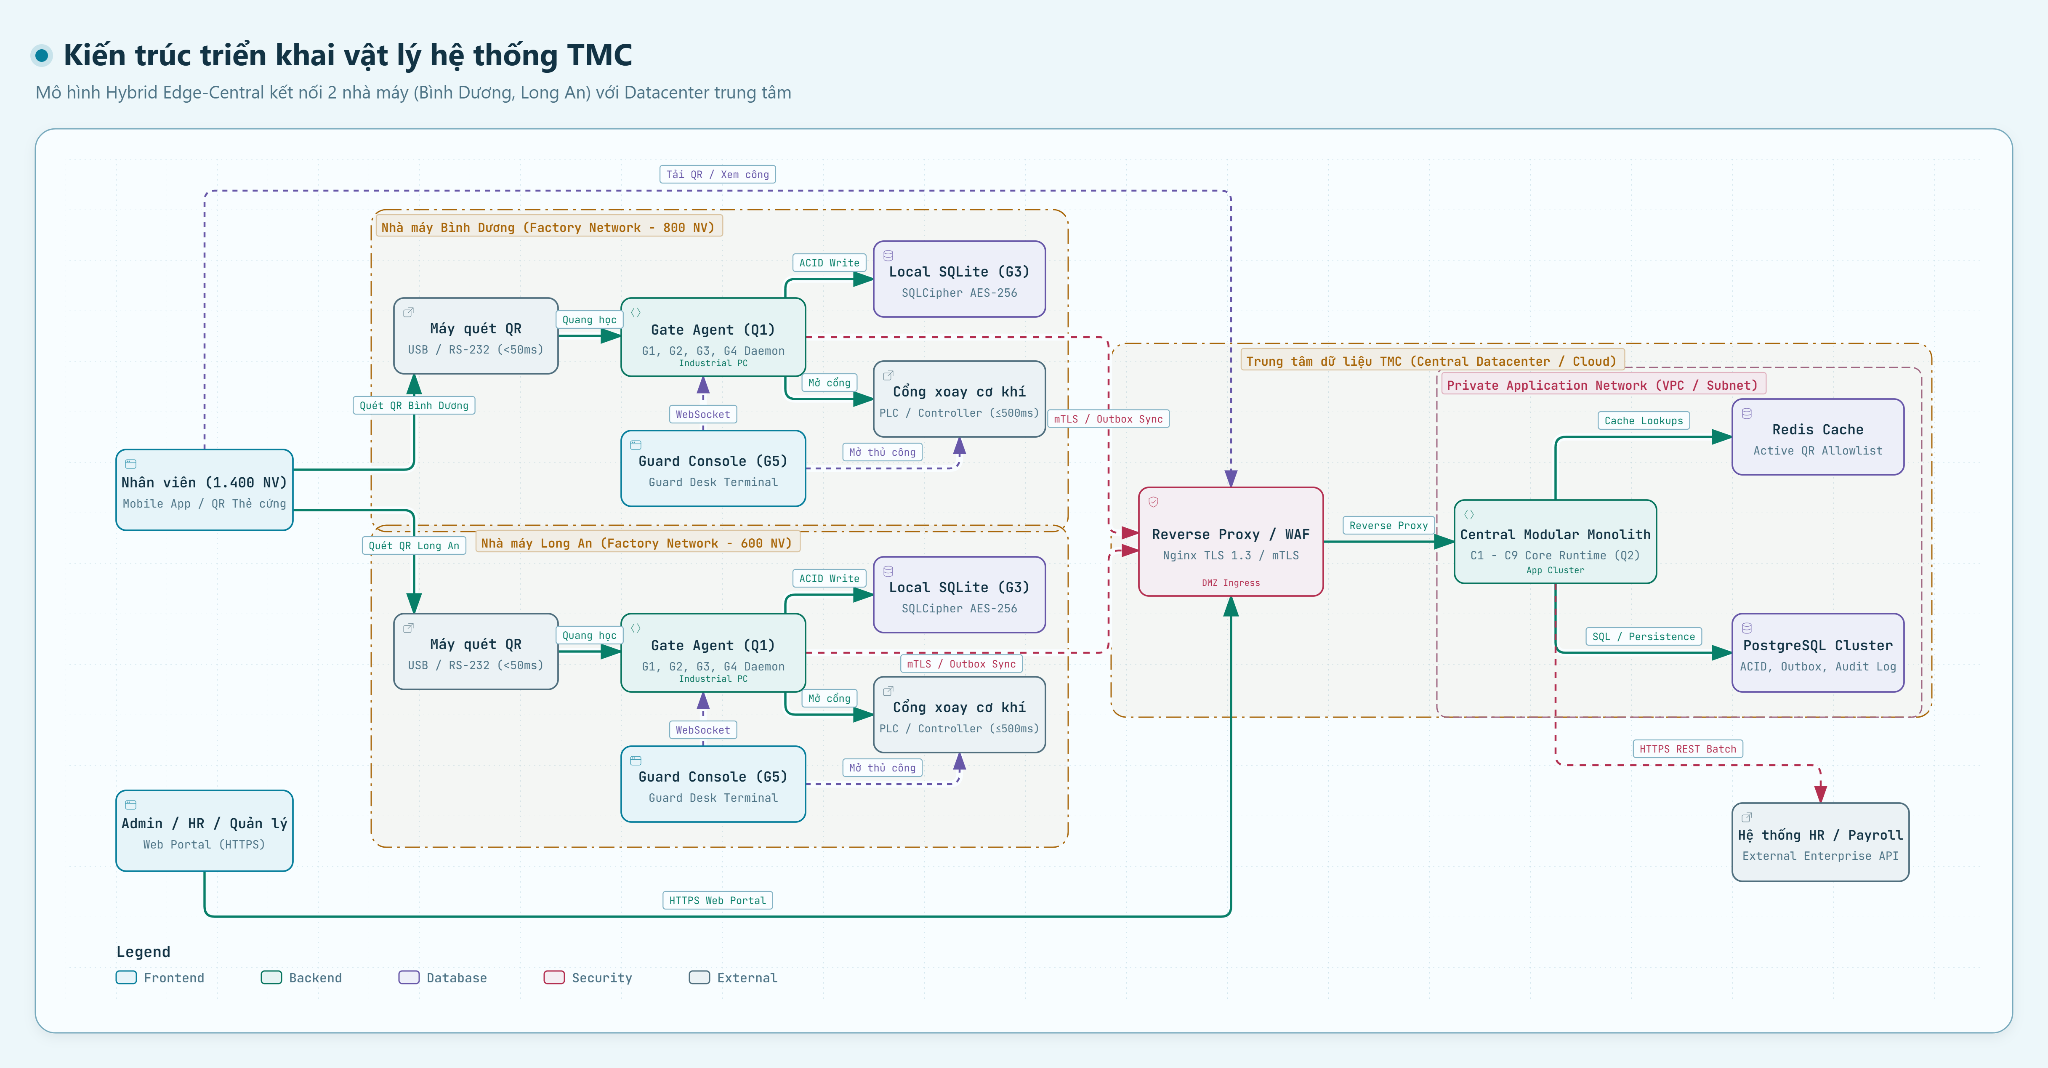
\includegraphics[width=0.95\textwidth]{figures/06_architecture_structure/deployment_diagram.png} 
\caption{Sơ đồ triển khai vật lý hệ thống TMC}
\end{figure}

\subsubsection{Đặc tả chi tiết các Node và Phân bổ Component}
Bảng dưới đây quy định chi tiết cấu hình phần cứng, vai trò môi trường và các component được triển khai trên từng nút mạng:

\small
\renewcommand{\arraystretch}{1.3}
\begin{longtable}{|>{\raggedright\arraybackslash}p{2.8cm}|>{\raggedright\arraybackslash}p{3.0cm}|>{\raggedright\arraybackslash}p{2.6cm}|>{\raggedright\arraybackslash}p{7.2cm}|}
\caption{Đặc tả chi tiết các Node và Phân bổ Component} \\
\hline
\textbf{Tên Node} & \textbf{Môi trường / Phần cứng} & \textbf{Component đảm nhận} & \textbf{Vai trò và Đặc tính kỹ thuật} \\
\hline
\endfirsthead

\hline
\textbf{Tên Node} & \textbf{Môi trường / Phần cứng} & \textbf{Component đảm nhận} & \textbf{Vai trò và Đặc tính kỹ thuật} \\
\hline
\endhead

\hline
\multicolumn{4}{r}{\textit{Còn tiếp sang trang sau...}} \\
\hline
\endfoot

\hline
\endlastfoot

Gate Station Kiosk Node (Tại mỗi cổng/nhà máy) & Industrial Mini PC (Linux Ubuntu Core / Alpine), RAM 4GB, 64GB SSD, Dual NIC (Ethernet). Gắn máy quét QR quang học và màn hình phụ. & G1 (Access Control), G2 (Turnstile Adapter), G3 (Local Store \& Outbox), G4 (Gate Sync Agent) & Chạy như một Service/Daemon độc lập trên Linux. Đảm bảo tính tự chủ tuyệt đối (DP-01). CSDL cục bộ dùng SQLite được mã hóa bằng SQLCipher (AES-256) để bảo vệ dữ liệu cục bộ (NFR-06). Giao tiếp quét mã qua cổng Serial RS-232 / USB HID với độ trễ $<$ 50ms. \\
\hline
Guard Desk Terminal (Tại phòng bảo vệ) & Máy tính bảng công nghiệp / PC màn hình cảm ứng, kết nối mạng LAN nội bộ nhà máy. & G5 (Guard Console - Web Frontend) & Ứng dụng Web tĩnh gọn nhẹ (Single Page Application) phục vụ giám sát luồng quẹt thẻ thời gian thực, hiển thị các bản ghi bị từ chối và thực hiện chức năng mở cổng thủ công khi xảy ra sự cố ngoại lệ (FR-09). \\
\hline
Turnstile Controller Node (Hệ thống ngoài) & Bộ điều khiển phần cứng của cổng xoay (PLC/Controller) do nhà cung cấp thiết bị lắp đặt. & Hệ thống Cổng xoay bên ngoài & Nhận tín hiệu điều khiển mở chốt cơ khí từ G2 qua giao thức TCP/IP Socket hoặc HTTP REST nội bộ LAN. Thời gian phản hồi phần cứng cam kết $\le$ 500ms (A-03). \\
\hline
DMZ Edge Gateway / Reverse Proxy (Trung tâm) & VM Linux cấu hình tối thiểu 2 vCPU, 4GB RAM, triển khai Nginx / HAProxy. & Reverse Proxy, SSL Termination, WAF & Đóng vai trò cổng vào duy nhất (Single Point of Ingress) cho Central Datacenter. Chấm dứt TLS 1.3, kiểm tra xác thực hai chiều mTLS đối với các Gate Agent (G4), định tuyến API và ngăn chặn tấn công DoS/DDoS. \\
\hline
Central Application Server Node (Trung tâm) & Cluster Container (Docker/K8s) hoặc VM Linux 4 vCPU, 8GB-16GB RAM. & C1 đến C9 (Central Modular Monolith) & Thực thi toàn bộ logic điều phối trung tâm. Triển khai theo mô hình Modular Monolith, các module giao tiếp In-process qua Application Events. Tách biệt thread pool giữa Ingestion (C1), Xử lý nghiệp vụ (C2, C3, C4) và Báo cáo (C6). \\
\hline
Central Database Server Node (Trung tâm) & Hệ quản trị CSDL Quan hệ PostgreSQL (Primary - Standby Replica). & Lưu trữ tập trung toàn bộ dữ liệu nghiệp vụ, Audit Log (C8), Read Model (C6) & Đảm bảo tính nhất quán mạnh (ACID) cho việc chốt kỳ, quản lý nhân viên, và lưu trữ lịch sử chấm công tập trung. Bảng audit\_log được cấu hình Append-Only và phân vùng theo thời gian (Partitioning by Month). \\
\hline
Central Cache Server Node (Trung tâm) & Redis Standalone / Cluster in-memory. & Cache danh mục QR hợp lệ, Session tài khoản RBAC & Tăng tốc độ đọc cho các tác vụ tra cứu QR của nhân viên và xác thực token JWT người dùng quản trị. \\
\end{longtable}
\normalsize

\subsubsection{Phân vùng mạng và Giao thức giao tiếp}
1. Mạng Cục bộ Nhà máy (Factory OT/LAN Network - Subnet riêng):
\begin{itemize}
    \item Kết nối giữa Kiosk và Turnstile Controller: Sử dụng mạng LAN cô lập vật lý hoặc VLAN chuyên dụng (VLAN IoT/OT). Giao thức điều khiển là HTTP/REST hoặc TCP Socket với địa chỉ IP tĩnh. Không cho phép truy cập Internet trực tiếp từ dải mạng này.
    \item Giao tiếp giữa G5 (Guard Console) và Kiosk: HTTP/WebSocket cục bộ qua LAN.
\end{itemize}

2. Mạng Diện rộng Kết nối Nhà máy - Trung tâm (WAN / VPN Tunnel):
\begin{itemize}
    \item Kênh truyền từ G4 (Gate Sync Agent) tại các nhà máy lên C1 (Gate Sync \& Ingestion) tại Trung tâm được bảo vệ thông qua đường truyền Site-to-Site IPSec VPN hoặc kênh mã hóa HTTPS/TLS 1.3 trên nền Internet công cộng.
    \item Cơ chế xác thực thiết bị: Sử dụng mTLS (Mutual TLS) với chứng chỉ số X.509 riêng biệt được nạp an toàn vào từng Kiosk phần cứng, ngăn chặn triệt để hành vi giả mạo Gate Agent để inject dữ liệu chấm công.
\end{itemize}

3. Mạng Tích hợp Hệ thống HR/Payroll:
\begin{itemize}
    \item C5 gọi sang API của Hệ thống HR/Payroll qua kênh truyền mạng riêng (Dedicated Leased Line / MPLS) hoặc HTTPS REST API bảo vệ bằng IP Whitelisting và OAuth 2.0 / Mutual TLS.
\end{itemize}
    \section{Quyết định kiến trúc hệ thống}\label{sec:architecture-decisions}
Mục này ghi nhận các quyết định kiến trúc (Architecture Decision Record -- ADR) định hình cách hệ thống TMC được xây dựng. ADR là quy tắc bắt buộc: một quyết định chỉ được thay đổi bằng một ADR mới thay thế nó. Mỗi ADR gồm bốn phần: bối cảnh, quyết định, hệ quả (lợi ích và đánh đổi) và các phương án thay thế đã được cân nhắc. Các ADR được xây dựng từ phân tích ở Mục~\ref{sec:architecture-structure} và chỉ sử dụng các yêu cầu, ràng buộc, bất biến đã được định nghĩa ở các phần trước.

\subsection{Bảng tổng hợp quyết định kiến trúc}\label{sec:adr-summary}

\begin{table}[H]
\centering
\caption{Tổng hợp quyết định kiến trúc}\label{tab:adr-summary}
\small
\renewcommand{\arraystretch}{1.3}
\begin{tabularx}{\textwidth}{|>{\centering\arraybackslash}p{1.4cm}|>{\raggedright\arraybackslash}X|>{\centering\arraybackslash}p{1.7cm}|>{\raggedright\arraybackslash}p{4.4cm}|>{\centering\arraybackslash}p{1.6cm}|}
\hline
\textbf{Mã} & \textbf{Quyết định} & \textbf{Trạng thái} & \textbf{Yêu cầu / ràng buộc liên quan} & \textbf{Mục liên quan} \\
\hline
ADR-01 & Topology triển khai kết hợp biên -- trung tâm, Gate Agent trên máy chủ biên của từng nhà máy & Accepted & NFR-PER-01, FR-17, NFR-AVL-04, NFR-REL-03, C-02, C-04, A-05 & \ref{sec:physical-step1} \\
\hline
ADR-02 & Mã QR động có chữ ký số, xác thực tại biên & Accepted & NFR-SEC-02, NFR-SEC-05, NFR-SEC-06, NFR-PER-01, R-04, R-06 & \ref{sec:quantum} \\
\hline
ADR-03 & Lưu bền vững tại cổng trước khi xác nhận và đồng bộ bằng transactional outbox & Accepted & NFR-REL-03, NFR-AVL-03, NFR-DIN-02, INV-05, INV-06, R-05 & \ref{sec:cc-views} \\
\hline
ADR-04 & Architecture style kết hợp: modular monolith tại trung tâm, microkernel và ports and adapters tại Gate Agent & Accepted & K1--K8; NFR-MOD-01 & \ref{sec:style-decision} \\
\hline
ADR-05 & Giao tiếp giữa hai quantum qua \textit{sync-contract} bất đồng bộ; giao tiếp trong Central qua interface và sự kiện trong tiến trình & Accepted & FR-17, NFR-SEC-06, NFR-DIN-02 & \ref{sec:logical-step4} \\
\hline
ADR-06 & Tích hợp cổng xoay và HR/Payroll qua adapter, có giới hạn thời gian chờ, circuit breaker và gửi lại & Accepted & C-01, C-02, NFR-REL-01, NFR-REL-02, NFR-INT-01 -- NFR-INT-04 & \ref{sec:logical-step4} \\
\hline
ADR-07 & Tổ chức mã nguồn: monorepo, phân chia theo module, kiểm thử kiến trúc tự động & Accepted & NFR-MOD-01, NFR-SCA-01 & \ref{sec:module-views} \\
\hline
ADR-08 & Kiểm soát truy cập, nhật ký kiểm toán bất biến và bảo vệ dữ liệu cá nhân & Accepted & C-03, NFR-SEC-01 -- NFR-SEC-04, NFR-AUD-01 -- NFR-AUD-05, NFR-PRI-01 -- NFR-PRI-04 & \ref{sec:physical-step4} \\
\hline
ADR-09 & Đồng bộ dữ liệu nhân viên từ HR/Payroll & Accepted & FR-01, NFR-SEC-06, NFR-INT-01 & \ref{sec:cc-views} \\
\hline
ADR-10 & Nền tảng công nghệ: Java và Spring Boot cho backend, React cho giao diện & Accepted & K6, K7; NFR-MOD-01 & \ref{sec:allocation-views} \\
\hline
\end{tabularx}
\end{table}

\subsection{Nội dung chi tiết các quyết định kiến trúc}

%------------------------------------------------------------------------------
\subsubsection{ADR-01: Topology triển khai kết hợp biên -- trung tâm}\label{adr:01}
\textbf{Trạng thái:} Accepted. \textbf{Nhóm:} cấu trúc, triển khai.

\noindent\textbf{1. Bối cảnh.} Hệ thống phục vụ hai nhà máy với khoảng 1.400 nhân viên. Giờ giao ca có khoảng 800 lượt quét trong 30 phút mỗi nhà máy, tương đương trung bình 0,44 lượt/giây và đỉnh giả định 2--5 lượt/giây mỗi nhà máy. Kiosk phải hiển thị kết quả trong 2 giây (NFR-PER-01) và cổng phải tiếp tục hoạt động khi mất kết nối với trung tâm (FR-17), trong khi đường truyền WAN giữa nhà máy và trung tâm có thể gián đoạn (R-02, A-05). Đồng thời, dữ liệu chấm công phải được tổng hợp tập trung để truyền sang HR/Payroll trước 12:00 ngày 1 (C-02).

\noindent\textbf{2. Quyết định.}
\begin{itemize}
    \item Áp dụng topology kết hợp biên -- trung tâm. Gate Agent (Gate Quantum) chạy trên \textbf{máy chủ biên của từng nhà máy} (Factory Edge Server), gồm một node chính và một node dự phòng nóng; kiosk tại trạm cổng chỉ là thiết bị đầu cuối không lưu dữ liệu.
    \item Central Quantum chạy tại trung tâm dữ liệu on-premise của TMC (A-05), trên \textbf{hai Central Application Server chạy song song} sau Reverse Proxy, cùng CSDL PostgreSQL có bản sao dự phòng.
    \item Toàn bộ đường xử lý lượt quét nằm trong mạng nhà máy; không có lời gọi đồng bộ nào qua WAN trên đường này.
\end{itemize}

\noindent\textbf{3. Hệ quả.}
\begin{itemize}
    \item \textit{Lợi ích:} cổng tiếp tục hoạt động khi mất kết nối với trung tâm; thời gian xử lý lượt quét không phụ thuộc chất lượng WAN; dữ liệu vẫn được quản lý tập trung; một kho cục bộ chung cho cả nhà máy bảo đảm quy tắc chống quẹt lặp chiều nhất quán (INV-04).
    \item \textit{Đánh đổi:} phải vận hành và cập nhật phần mềm cho các node tại nhà máy; dữ liệu giữa hai quantum chỉ nhất quán cuối cùng (độ trễ $\le$ 60 giây); thiết bị đặt tại hiện trường cần được bảo vệ (mã hóa dữ liệu, chứng chỉ thiết bị -- ADR-08). Central phải chạy hai node vì việc cấp mã QR động nằm trên đường đi của nhân viên (ADR-02).
\end{itemize}

\noindent\textbf{4. Phương án thay thế.}
\begin{itemize}
    \item \textit{Tập trung hoàn toàn:} bị loại vì mỗi lượt quét phụ thuộc WAN, vi phạm FR-17 khi mất kết nối.
    \item \textit{Phân tán hoàn toàn tại từng nhà máy:} bị loại vì dữ liệu, tài khoản và audit bị phân mảnh, khó đáp ứng C-02.
    \item \textit{Gate Agent chạy trên từng kiosk:} bị loại vì quy tắc chống quẹt lặp chiều phải đồng bộ ngang giữa các kiosk, số node cần quản lý và bảo vệ tăng theo số trạm.
\end{itemize}

%------------------------------------------------------------------------------
\subsubsection{ADR-02: Mã QR động có chữ ký số, xác thực tại biên}\label{adr:02}
\textbf{Trạng thái:} Accepted. \textbf{Nhóm:} bảo mật, hiệu năng.

\noindent\textbf{1. Bối cảnh.} Mã QR tĩnh có thể bị chụp lại, chia sẻ hoặc phát lại để ra vào trái phép hoặc chấm công hộ (R-06). Trạng thái thu hồi lưu tại trạm cổng có thể chưa kịp cập nhật (R-04), nhất là khi mất kết nối. Mặt khác, việc xác thực phải hoàn tất tại cổng, không gọi trung tâm (ADR-01), và nằm trong ngân sách 2 giây (NFR-PER-01). Mọi nhân viên đều có điện thoại để mở TMC Employee Portal (A-02).

\noindent\textbf{2. Quyết định.}
\begin{itemize}
    \item Mã QR hiển thị cho nhân viên là một token gồm phiên bản, mã credential, thời điểm phát hành, thời điểm hết hạn, một giá trị ngẫu nhiên dùng một lần (nonce) và mã định danh khóa, được ký bằng \textbf{Ed25519}. Thời hạn hiệu lực không quá 60 giây (NFR-SEC-05); Portal lấy mã mới khoảng mỗi 30 giây qua \texttt{QrTokenAPI} của C2.
    \item Khóa bí mật chỉ nằm tại Central (C2). Gate Agent chỉ nhận khóa công khai qua chiều đồng bộ xuống.
    \item G1 xác thực mã hoàn toàn bằng dữ liệu cục bộ: kiểm tra chữ ký, thời hạn (cho phép lệch đồng hồ $\pm$30 giây, các node đồng bộ thời gian qua NTP), nonce chưa được sử dụng, credential đang hiệu lực, nhân viên đang hoạt động, trạm đang bật và quy tắc chống quẹt lặp chiều.
    \item Khóa ký được thay theo chu kỳ; mã định danh khóa cho phép khóa cũ và khóa mới được chấp nhận song song trong thời gian chuyển đổi.
\end{itemize}

\noindent\textbf{3. Hệ quả.}
\begin{itemize}
    \item \textit{Lợi ích:} ảnh chụp mã QR chỉ dùng được trong thời hạn ngắn và chỉ một lần; thu hồi có hiệu lực gần như ngay lập tức kể cả khi trạm đang mất kết nối, vì Portal không cấp mã mới cho credential đã thu hồi; thiết bị tại nhà máy bị đánh cắp cũng không thể tạo mã hợp lệ; xác thực chỉ mất vài mili-giây.
    \item \textit{Đánh đổi:} việc cấp mã phụ thuộc Central, nên Central phải có hai node chạy song song (ADR-01); điện thoại của nhân viên cần kết nối mạng để lấy mã, nếu không thì bảo vệ mở cổng thủ công (FR-10); các node phải đồng bộ thời gian; cần quy trình quản lý và thay khóa.
\end{itemize}

\noindent\textbf{4. Phương án thay thế.}
\begin{itemize}
    \item \textit{Mã QR tĩnh có chữ ký (HMAC):} bị loại vì mã bị lộ dùng được vô thời hạn và khóa bí mật phải đặt tại trạm cổng.
    \item \textit{Mã TOTP sinh trên điện thoại:} không chọn vì cần ứng dụng di động lưu khóa bí mật trên thiết bị của nhân viên; có thể xem xét trong tương lai.
    \item \textit{Tra cứu trung tâm ở mỗi lượt quét:} bị loại vì phụ thuộc WAN (vi phạm ADR-01, FR-17).
\end{itemize}

%------------------------------------------------------------------------------
\subsubsection{ADR-03: Lưu bền vững tại cổng trước khi xác nhận và đồng bộ bằng transactional outbox}\label{adr:03}
\textbf{Trạng thái:} Accepted. \textbf{Nhóm:} độ tin cậy, toàn vẹn dữ liệu.

\noindent\textbf{1. Bối cảnh.} Hệ thống không được làm mất giao dịch chấm công (NFR-REL-03), không được báo mở cổng thành công khi cổng xoay chưa xác nhận (NFR-AVL-03), và không được để xảy ra trường hợp cổng đã mở nhưng không có dấu vết hoặc giao dịch bị ghi trùng (R-05). Kết nối giữa nhà máy và trung tâm có thể gián đoạn bất kỳ lúc nào.

\noindent\textbf{2. Quyết định.}
\begin{itemize}
    \item Trình tự xử lý tại Gate Agent (luồng F1): (1) xác thực; (2) ghi bền vững lượt quét ở trạng thái chờ xác nhận; (3) gọi cổng xoay; (4) chỉ khi cổng xác nhận mở mới ghi giao dịch chấm công và bản ghi outbox trong cùng một giao dịch cục bộ, rồi báo thành công; (5) nếu cổng không phản hồi hoặc báo lỗi, lượt quét được đánh dấu mở cổng thất bại và kiosk không báo thành công.
    \item Khi Gate Agent khởi động lại, các lượt quét còn ở trạng thái chờ xác nhận được đưa lên bảng điều khiển của bảo vệ để đối soát.
    \item G4 gửi các bản ghi outbox theo lô lên C1; C1 lưu idempotent theo mã sự kiện (INV-06); G4 chỉ đánh dấu đã đồng bộ sau khi nhận xác nhận từ C1.
\end{itemize}

\noindent\textbf{3. Hệ quả.}
\begin{itemize}
    \item \textit{Lợi ích:} không mất dấu vết kể cả khi mất nguồn giữa chừng; không có giao dịch chấm công cho lượt cổng không mở; dữ liệu được chuyển giao ít nhất một lần và không trùng lặp.
    \item \textit{Đánh đổi:} mỗi lượt quét có hai lần ghi đĩa đồng bộ (khoảng 50 ms mỗi lần, nằm trong ngân sách ở Bảng~\ref{tab:time-budget}); máy chủ biên cần SSD công nghiệp; cần cơ chế đối soát lượt quét chờ xác nhận.
\end{itemize}

\noindent\textbf{4. Phương án thay thế.}
\begin{itemize}
    \item \textit{Mở cổng trước, ghi dữ liệu sau vào bộ nhớ:} bị loại vì mất dữ liệu khi mất nguồn (vi phạm NFR-REL-03).
    \item \textit{Ghi giao dịch trước khi mở cổng:} bị loại vì tạo giao dịch cho lượt cổng không mở được và phải báo thành công trước khi cổng xác nhận (vi phạm NFR-AVL-03, R-05).
    \item \textit{Giao dịch phân tán (two-phase commit) giữa cổng và trung tâm:} bị loại vì không hoạt động khi mất kết nối.
\end{itemize}

%------------------------------------------------------------------------------
\subsubsection{ADR-04: Architecture style kết hợp}\label{adr:04}
\textbf{Trạng thái:} Accepted. \textbf{Nhóm:} cấu trúc.

\noindent\textbf{1. Bối cảnh.} Phân tích quantum (Mục~\ref{sec:quantum}) cho thấy hệ thống cần hai loại đơn vị triển khai độc lập. Việc đánh giá các style theo tiêu chí K1--K8 (Mục~\ref{sec:style-evaluation}) cho thấy không style đơn lẻ nào đáp ứng tốt đồng thời yêu cầu hoạt động khi mất kết nối (K4) và chi phí, năng lực của nhóm (K6, K7).

\noindent\textbf{2. Quyết định.}
\begin{itemize}
    \item Central Quantum là \textbf{modular monolith}: một đơn vị triển khai gồm các module C1--C9, mỗi module sở hữu dữ liệu của mình và chỉ giao tiếp với module khác qua interface công khai hoặc sự kiện trong tiến trình.
    \item Gate Agent áp dụng \textbf{microkernel kết hợp ports and adapters}: lõi xử lý xác thực và lưu trữ; thiết bị quét và cổng xoay của từng nhà cung cấp được cắm vào qua adapter cài đặt interface do lõi định nghĩa.
    \item Hai quantum liên kết bằng transactional outbox (ADR-03, ADR-05), không dùng message broker.
\end{itemize}

\noindent\textbf{3. Hệ quả.}
\begin{itemize}
    \item \textit{Lợi ích:} giữ giao dịch ACID cho các bất biến tại trung tâm (INV-01, INV-08, INV-09); chi phí vận hành thấp vì chỉ có hai loại đơn vị triển khai; thay nhà cung cấp cổng xoay chỉ cần thêm adapter (NFR-MOD-01).
    \item \textit{Đánh đổi:} cần kỷ luật giữ ranh giới module, được kiểm tra tự động (ADR-07); nâng cấp một module tại trung tâm phải triển khai lại toàn bộ Central, điều này chấp nhận được vì cổng vẫn hoạt động độc lập.
\end{itemize}

\noindent\textbf{4. Phương án thay thế.} Layered (55 điểm), modular monolith đơn thuần (65), microkernel (59), service-based với 4--6 dịch vụ (72), event-driven có broker (63) và microservices (54) đều được đánh giá thấp hơn phương án kết hợp (85) theo Bảng~\ref{tab:style-scores}.

%------------------------------------------------------------------------------
\subsubsection{ADR-05: Giao tiếp giữa hai quantum và bên trong Central}\label{adr:05}
\textbf{Trạng thái:} Accepted. \textbf{Nhóm:} giao tiếp.

\noindent\textbf{1. Bối cảnh.} Hệ thống có hai loại ranh giới giao tiếp: giữa Gate Quantum và Central Quantum qua WAN, và giữa các module bên trong Central. Giao tiếp giữa hai quantum không được làm chậm luồng quét và phải chịu được mất kết nối; giao tiếp bên trong Central phải giữ ghép nối lỏng và không có vòng phụ thuộc.

\noindent\textbf{2. Quyết định.}
\begin{itemize}
    \item Giữa hai quantum chỉ dùng hợp đồng dữ liệu \textit{sync-contract} có quản lý phiên bản, truyền bằng \textbf{REST/JSON qua HTTPS}. Chiều lên: G4 gửi lô sự kiện từ outbox, idempotent theo mã sự kiện. Chiều xuống: G4 định kỳ kéo phần thay đổi của credential, khóa công khai và cấu hình trạm, bảo đảm độ trễ $\le$ 60 giây (NFR-SEC-06); thay đổi thu hồi credential được ưu tiên.
    \item Bên trong Central: truy vấn qua interface công khai của module; thông báo thay đổi trạng thái qua sự kiện trong tiến trình. Chiều phụ thuộc giữa các module phải không có vòng (Mục~\ref{sec:module-views}); để giữ quy tắc này, C1 gọi interface của C3 và C5 gọi interface của C2 thay vì phát sự kiện ngược chiều.
\end{itemize}

\noindent\textbf{3. Hệ quả.}
\begin{itemize}
    \item \textit{Lợi ích:} Central có thể bảo trì mà không dừng cổng; module phát sự kiện không cần biết module nhận; REST/JSON dễ kiểm thử và gỡ lỗi.
    \item \textit{Đánh đổi:} dữ liệu giữa các quantum và read model báo cáo chỉ nhất quán cuối cùng; phải quản lý phiên bản \textit{sync-contract} để Gate Agent và Central khác phiên bản vẫn tương thích trong thời gian nâng cấp.
\end{itemize}

\noindent\textbf{4. Phương án thay thế.}
\begin{itemize}
    \item \textit{Message broker (Kafka, RabbitMQ):} bị loại vì quá mức cần thiết với tải vài sự kiện mỗi giây và thêm thành phần cần vận hành, bảo mật.
    \item \textit{Chia sẻ CSDL giữa hai quantum:} bị loại vì không hoạt động khi mất kết nối và phá ranh giới quantum.
    \item \textit{gRPC:} không chọn vì REST/JSON đủ đáp ứng tải hiện tại và đơn giản hơn cho việc kiểm thử, giám sát.
\end{itemize}

%------------------------------------------------------------------------------
\subsubsection{ADR-06: Tích hợp cổng xoay và HR/Payroll qua adapter}\label{adr:06}
\textbf{Trạng thái:} Accepted. \textbf{Nhóm:} tích hợp, chịu lỗi.

\noindent\textbf{1. Bối cảnh.} Hệ thống phải tích hợp với hệ thống cổng xoay và hệ thống HR/Payroll qua API (C-01), cả hai nằm ngoài tầm kiểm soát của nhóm. Cổng xoay có thể không phản hồi hoặc báo lỗi; HR/Payroll có thể tạm thời không khả dụng đúng lúc truyền dữ liệu cuối tháng (R-03, C-02).

\noindent\textbf{2. Quyết định.}
\begin{itemize}
    \item \textbf{Cổng xoay:} domain của G1 định nghĩa port \texttt{TurnstileGateway}; mỗi nhà cung cấp có một adapter trong G2. Lời gọi mở cổng có giới hạn thời gian chờ 800 ms, lớn hơn thời gian phản hồi cam kết 500 ms (A-04). Khi hết thời gian chờ, G2 kiểm tra trạng thái cổng trước khi gửi lại lệnh (NFR-REL-02); không gửi lại theo backoff để tránh mở cổng hai lần. Sau năm lỗi liên tiếp, circuit breaker ngừng gửi lệnh tự động và cảnh báo bảo vệ để mở cổng thủ công (FR-10).
    \item \textbf{HR/Payroll:} C5 cài đặt hai port \texttt{HrPayroll\-Gateway} (gửi đợt dữ liệu chấm công) và \texttt{Employee\-Source\-Gateway} (nhận dữ liệu nhân viên, ADR-09). Đợt truyền được gửi bất đồng bộ, gửi lại theo exponential backoff (1, 2, 4, 8 phút\ldots) khi lỗi tạm thời (NFR-REL-01), idempotent theo mã đợt (NFR-INT-04). Nhân viên HR có thể theo dõi và gửi lại thủ công (FR-22); hệ thống cảnh báo khi gần hạn 12:00 ngày 1 mà đợt chính chưa được xác nhận.
\end{itemize}

\noindent\textbf{3. Hệ quả.}
\begin{itemize}
    \item \textit{Lợi ích:} sự cố của hệ thống bên ngoài không làm treo luồng quét hay nghiệp vụ chốt kỳ; thay nhà cung cấp hoặc API bên ngoài chỉ cần thay adapter (NFR-MOD-01); adapter có thể thay bằng bản giả lập khi kiểm thử.
    \item \textit{Đánh đổi:} khi circuit breaker ngắt, việc ra vào tại trạm đó phụ thuộc thao tác thủ công của bảo vệ; cần màn hình theo dõi trạng thái truyền và cơ chế cảnh báo.
\end{itemize}

\noindent\textbf{4. Phương án thay thế.}
\begin{itemize}
    \item \textit{Gọi trực tiếp API bên ngoài trong mã nghiệp vụ:} bị loại vì làm nghiệp vụ phụ thuộc vào API bên ngoài (vi phạm NFR-MOD-01).
    \item \textit{Ghi trực tiếp vào CSDL của HR/Payroll:} bị loại vì vi phạm ranh giới hệ thống và có rủi ro về toàn vẹn dữ liệu của hệ thống HR/Payroll.
\end{itemize}

%------------------------------------------------------------------------------
\subsubsection{ADR-07: Tổ chức mã nguồn và kiểm thử kiến trúc}\label{adr:07}
\textbf{Trạng thái:} Accepted. \textbf{Nhóm:} phát triển, khả năng sửa đổi.

\noindent\textbf{1. Bối cảnh.} Hệ thống gồm hai ứng dụng triển khai riêng (\texttt{gate-agent}, \texttt{central}) dùng chung hợp đồng \textit{sync-contract}. Nhóm phát triển nhỏ cần đồng bộ thay đổi trên hợp đồng này một cách dễ dàng, đồng thời cấu trúc mã nguồn phải phản ánh ranh giới domain để tránh suy thoái kiến trúc theo thời gian.

\noindent\textbf{2. Quyết định.}
\begin{itemize}
    \item Toàn bộ mã nguồn nằm trong một kho mã (monorepo) \texttt{tmc}, gồm \texttt{sync-contract}, \texttt{gate-agent}, \texttt{central}, mã nguồn giao diện \texttt{web} và cấu hình triển khai \texttt{deploy} (Bảng~\ref{tab:implementation-view}).
    \item Mã nguồn được chia package theo module (package-by-feature), mỗi module ứng với một component; bên trong mỗi module có bốn tầng \texttt{api}, \texttt{application}, \texttt{domain}, \texttt{infrastructure} (Mục~\ref{sec:module-views}).
    \item Các quy tắc phụ thuộc ở Mục~\ref{sec:module-views} được kiểm tra tự động bằng ArchUnit trong quy trình tích hợp liên tục (CI); vi phạm làm build thất bại.
    \item Tham số thay đổi theo nhà máy hoặc môi trường (ngưỡng mất kết nối, giới hạn thời gian chờ, chu kỳ đồng bộ) được nạp từ cấu hình (C9 hoặc biến môi trường), không viết cứng trong mã.
\end{itemize}

\noindent\textbf{3. Hệ quả.}
\begin{itemize}
    \item \textit{Lợi ích:} một thay đổi có thể cập nhật đồng thời \textit{sync-contract}, phía gửi và phía nhận; các thành viên làm việc song song trên các module khác nhau; ranh giới kiến trúc được giữ bằng kiểm thử tự động thay vì chỉ dựa vào kỷ luật.
    \item \textit{Đánh đổi:} kho mã lớn dần; CI cần được cấu hình để chỉ build và kiểm thử phần bị thay đổi.
\end{itemize}

\noindent\textbf{4. Phương án thay thế.}
\begin{itemize}
    \item \textit{Mỗi ứng dụng một kho mã:} bị loại vì việc quản lý phiên bản hợp đồng dùng chung phức tạp với nhóm nhỏ.
    \item \textit{Chia package theo tầng kỹ thuật (controller, service, repository):} bị loại vì phá vỡ ranh giới domain và không khớp với cách phân rã đã chọn (Mục~\ref{sec:partitioning}).
\end{itemize}

%------------------------------------------------------------------------------
\subsubsection{ADR-08: Kiểm soát truy cập, nhật ký kiểm toán bất biến và bảo vệ dữ liệu cá nhân}\label{adr:08}
\textbf{Trạng thái:} Accepted. \textbf{Nhóm:} bảo mật, quyền riêng tư.

\noindent\textbf{1. Bối cảnh.} Hệ thống xử lý dữ liệu cá nhân của nhân viên (họ tên, mã nhân viên, bộ phận, lịch sử ra vào) và phải tuân thủ quy định về bảo vệ dữ liệu cá nhân (C-03, Nghị định 13/2023/NĐ-CP). Mọi chức năng được bảo vệ phải kiểm tra quyền (NFR-SEC-01), mọi thao tác quan trọng phải để lại nhật ký không thể sửa xóa (NFR-AUD-01 -- NFR-AUD-05), và thiết bị đặt tại nhà máy có thể bị can thiệp.

\noindent\textbf{2. Quyết định.}
\begin{itemize}
    \item \textbf{Kiểm soát truy cập:} C7 quản lý tài khoản, vai trò và quyền. Mọi API của Central yêu cầu token có chữ ký (JWT, thuật toán RS256) và kiểm tra quyền ở cả mức chức năng và mức dữ liệu; giám sát sản xuất chỉ xem được nhân viên thuộc bộ phận mình phụ trách (FR-19, INV-11).
    \item \textbf{Thiết bị:} kiosk không yêu cầu tài khoản người dùng. Mỗi Gate Agent có chứng chỉ thiết bị riêng để xác thực hai chiều (mTLS) với trung tâm; chứng chỉ của thiết bị bị mất được thu hồi.
    \item \textbf{Bảo vệ đăng nhập khi mất kết nối:} thông tin xác thực (dạng băm) và quyền mở cổng thủ công của các tài khoản bảo vệ được đồng bộ xuống Gate Agent; thao tác mở cổng thủ công được ghi nhật ký cục bộ và đồng bộ lên C8.
    \item \textbf{Bảo vệ dữ liệu:} bản sao tại Gate Agent chỉ chứa dữ liệu cần cho xác thực (mã credential, mã nhân viên, trạng thái); CSDL cục bộ được mã hóa; CSDL trung tâm được mã hóa khi lưu. Kết nối qua WAN và tới trung tâm dùng TLS $\ge$ 1.2, ưu tiên 1.3; kết nối tới cổng xoay theo hợp đồng của nhà cung cấp trong VLAN cô lập (NFR-SEC-03). Khóa bí mật ký mã QR chỉ nằm trong kho khóa của trung tâm (ADR-02).
    \item \textbf{Nhật ký kiểm toán:} C8 chỉ cho phép thêm bản ghi, không tài khoản ứng dụng nào có quyền sửa hoặc xóa; mỗi bản ghi lưu giá trị băm của bản ghi trước để phát hiện can thiệp trực tiếp vào CSDL; dữ liệu được lưu trực tuyến tối thiểu 12 tháng trước khi chuyển sang kho lưu trữ dài hạn (INV-10).
\end{itemize}

\noindent\textbf{3. Hệ quả.}
\begin{itemize}
    \item \textit{Lợi ích:} đáp ứng yêu cầu pháp lý và yêu cầu kiểm toán; thiết bị tại nhà máy bị đánh cắp không làm lộ dữ liệu và không thể dùng để gửi dữ liệu giả hay tạo mã QR; nhật ký kiểm toán là bằng chứng tin cậy khi giải quyết khiếu nại.
    \item \textit{Đánh đổi:} mã hóa làm tăng nhẹ thời gian đọc ghi; cần quy trình quản lý chứng chỉ và khóa; bảng nhật ký lớn dần theo thời gian, cần phân vùng theo tháng.
\end{itemize}

\noindent\textbf{4. Phương án thay thế.}
\begin{itemize}
    \item \textit{Ghi nhật ký vào tệp văn bản:} bị loại vì dễ bị sửa hoặc xóa bởi người có quyền quản trị máy chủ.
    \item \textit{Lưu đầy đủ hồ sơ nhân viên tại kiosk để hiển thị:} bị loại vì làm tăng rủi ro lộ dữ liệu cá nhân tại hiện trường.
\end{itemize}

%------------------------------------------------------------------------------
\subsubsection{ADR-09: Đồng bộ dữ liệu nhân viên từ HR/Payroll}\label{adr:09}
\textbf{Trạng thái:} Accepted. \textbf{Nhóm:} tích hợp, toàn vẹn dữ liệu.

\noindent\textbf{1. Bối cảnh.} HR/Payroll là nguồn dữ liệu nhân sự chính thức; hệ thống TMC chỉ tiếp nhận và đồng bộ, không tự tạo dữ liệu nhân sự gốc (Mục~\ref{sec:external-boundaries}, FR-01). Khi nhân viên nghỉ việc, QR credential phải bị thu hồi kịp thời (NFR-SEC-06). Khả năng API của HR/Payroll cần được xác nhận (A-03).

\noindent\textbf{2. Quyết định.}
\begin{itemize}
    \item C5 định kỳ (mặc định 15 phút, cấu hình tại C9) lấy phần thay đổi dữ liệu nhân viên qua port \texttt{Employee\-Source\-Gateway}, rồi gọi interface của C2 để cập nhật hồ sơ theo mã nhân viên; việc cập nhật là idempotent nên chạy lại không tạo dữ liệu trùng.
    \item Khi nhân viên chuyển sang trạng thái không hoạt động, C2 thu hồi QR credential đang hiệu lực và thay đổi được phát xuống các trạm theo luồng đồng bộ chiều xuống.
    \item Khi API của HR/Payroll chưa sẵn sàng, nhân viên HR có thể cập nhật thủ công; mọi cập nhật được ghi nhật ký kiểm toán.
\end{itemize}

\noindent\textbf{3. Hệ quả.}
\begin{itemize}
    \item \textit{Lợi ích:} một nguồn dữ liệu nhân sự duy nhất, tránh lệch dữ liệu giữa hai hệ thống; việc thu hồi credential khi nhân viên nghỉ việc diễn ra tự động.
    \item \textit{Đánh đổi:} có độ trễ tối đa bằng chu kỳ đồng bộ giữa HR/Payroll và TMC; phụ thuộc vào khả năng cung cấp dữ liệu thay đổi của API HR/Payroll.
\end{itemize}

\noindent\textbf{4. Phương án thay thế.}
\begin{itemize}
    \item \textit{Nhập dữ liệu thủ công hoặc qua tệp CSV:} bị loại làm phương án chính vì chậm và dễ sai; chỉ dùng làm phương án dự phòng.
    \item \textit{HR/Payroll chủ động đẩy thay đổi sang TMC (webhook):} không chọn vì phụ thuộc vào khả năng của hệ thống hiện có, chưa được xác nhận (A-03).
    \item \textit{Đọc trực tiếp CSDL của HR/Payroll:} bị loại vì vi phạm ranh giới hệ thống.
\end{itemize}

%------------------------------------------------------------------------------
\subsubsection{ADR-10: Nền tảng công nghệ}\label{adr:10}
\textbf{Trạng thái:} Accepted. \textbf{Nhóm:} công nghệ.

\noindent\textbf{1. Bối cảnh.} Kiến trúc đã chọn cần một nền tảng hỗ trợ tốt việc tổ chức module, interface và kiểm thử kiến trúc (ADR-04, ADR-07), chạy được trên máy chủ biên và máy chủ trung tâm, phù hợp với năng lực của nhóm (K7) và có chi phí vận hành thấp (K6).

\noindent\textbf{2. Quyết định.}
\begin{itemize}
    \item \textbf{Backend:} Java 21 và Spring Boot 3 cho cả \texttt{gate-agent} và \texttt{central}; \textit{sync-contract} là thư viện Java dùng chung. Central dùng Spring Modulith để kiểm tra ranh giới module, phát sự kiện trong tiến trình và lưu sự kiện chưa xử lý (dùng làm outbox trung tâm).
    \item \textbf{Giao diện:} React cho giao diện kiosk, bảng điều khiển của bảo vệ và giao diện quản trị; bản build tĩnh được đóng gói vào artifact \texttt{gate-agent} hoặc \texttt{central} tương ứng.
    \item \textbf{Lưu trữ:} SQLite được mã hóa tại Gate Agent, truy cập qua JDBC; PostgreSQL tại Central, truy cập qua Spring Data JPA.
    \item \textbf{Hạ tầng và thư viện khác:} container cho cả hai loại node; Nginx làm reverse proxy; thuật toán Ed25519 có sẵn trong JDK để ký và kiểm tra mã QR; ArchUnit cho kiểm thử kiến trúc.
\end{itemize}

\noindent\textbf{3. Hệ quả.}
\begin{itemize}
    \item \textit{Lợi ích:} một ngôn ngữ cho toàn bộ backend; hệ sinh thái Spring hỗ trợ sẵn tiêm phụ thuộc, giao dịch, sự kiện và kiểm thử, phù hợp với ports and adapters; Spring Modulith và ArchUnit giúp giữ ranh giới kiến trúc; SQLite không cần cài đặt máy chủ CSDL tại nhà máy.
    \item \textit{Đánh đổi:} ứng dụng Java tiêu tốn bộ nhớ hơn và khởi động chậm hơn, chấp nhận được với cấu hình máy chủ biên ở Bảng~\ref{tab:nodes}; nhóm phải làm việc với hai ngôn ngữ (Java cho backend, JavaScript/TypeScript cho React).
\end{itemize}

\noindent\textbf{4. Phương án thay thế.}
\begin{itemize}
    \item \textit{TypeScript với NestJS cho backend:} không chọn; ưu điểm là dùng một ngôn ngữ cho cả backend và giao diện, nhưng công cụ kiểm thử kiến trúc và quản lý module kém hơn hệ sinh thái Java, và không phù hợp năng lực hiện có của nhóm.
    \item \textit{Python với FastAPI:} bị loại vì kiểu động khiến việc thể hiện và kiểm tra interface, ranh giới module khó hơn.
    \item \textit{CSDL máy chủ (PostgreSQL) tại nhà máy:} không chọn vì tăng chi phí vận hành tại hiện trường trong khi tải tại nhà máy thấp.
\end{itemize}

    \section{Nguyên lý thiết kế hệ thống}\label{sec:design-principles}

\subsection{Tổng quan}\label{sec:dp-overview}
\begin{table}[H]
\centering
\caption{Các nhóm nguyên tắc thiết kế}\label{tab:dp-groups}
\small
\renewcommand{\arraystretch}{1.3}
\begin{tabularx}{\textwidth}{|>{\raggedright\arraybackslash}p{4.6cm}|>{\raggedright\arraybackslash}p{3.8cm}|>{\raggedright\arraybackslash}X|}
\hline
\textbf{Nhóm} & \textbf{Đặc tính phục vụ} & \textbf{Nguyên tắc} \\
\hline
Độ tin cậy và toàn vẹn dữ liệu & Reliability, Data Integrity & DP-01 -- DP-04 \\
\hline
Hiệu năng và tự chủ khi mất kết nối & Performance, Availability & DP-05 -- DP-09 \\
\hline
Bảo mật và bảo vệ dữ liệu cá nhân & Security, Privacy, Auditability & DP-10 -- DP-13 \\
\hline
Tính module và khả năng sửa đổi & Modifiability, Scalability & DP-14 -- DP-17 \\
\hline
\end{tabularx}
\end{table}

%==============================================================================
\subsection{Nhóm nguyên tắc về độ tin cậy và toàn vẹn dữ liệu}\label{sec:dp-reliability}
Nhóm này phục vụ hai trong ba đặc tính dẫn dắt của hệ thống (Mục~\ref{sec:top3}): không để mất và không để sai lệch dữ liệu chấm công.

\paragraph{DP-01. Lưu bền vững trước khi xác nhận.}\label{dp:01}
\begin{itemize}
    \item \textit{Phát biểu:} Không thông báo thành công cho một thao tác khi dữ liệu của thao tác đó chưa được lưu bền vững, hoặc khi bên thực hiện cuối cùng chưa xác nhận.
    \item \textit{Lý do:} NFR-REL-03, NFR-AVL-03, INV-05; Reliability.
    \item \textit{Áp dụng trong TMC:} trong luồng F1, G1 ghi lượt quét ở trạng thái chờ xác nhận trước khi gọi cổng xoay, và chỉ ghi giao dịch chấm công cùng bản ghi outbox khi cổng đã xác nhận mở (ADR-03). C4 ghi đợt truyền trước khi C5 gửi đi; kỳ chỉ chuyển sang LOCKED khi HR/Payroll xác nhận.
    \item \textit{Trường hợp linh hoạt:} dữ liệu có thể dựng lại được, như read model của C6 hoặc heartbeat, không cần ghi trước khi xử lý.
\end{itemize}

\paragraph{DP-02. Dữ kiện bất biến, sửa bằng bản ghi mới.}\label{dp:02}
\begin{itemize}
    \item \textit{Phát biểu:} Dữ kiện đã ghi nhận (giao dịch chấm công, nhật ký kiểm toán) không bị sửa hay xóa; mọi thay đổi được thể hiện bằng một bản ghi mới tham chiếu tới bản ghi gốc.
    \item \textit{Lý do:} INV-08, INV-10; NFR-DIN-03; Data Integrity, Auditability.
    \item \textit{Áp dụng trong TMC:} AttendanceTransaction và AuditLogEntry chỉ được ghi thêm; việc sửa chấm công dùng AttendanceAdjustment; sau khi kỳ chuyển sang LOCKED, thay đổi được gửi qua đợt truyền bổ sung (INV-09). ScanAttempt chỉ được đổi trạng thái theo đúng vòng đời: chờ xác nhận, rồi được chấp nhận hoặc mở cổng thất bại.
    \item \textit{Trường hợp linh hoạt:} dữ liệu danh mục như hồ sơ nhân viên và cấu hình trạm được cập nhật tại chỗ, nhưng mỗi thay đổi phải được ghi nhật ký kiểm toán.
\end{itemize}

\paragraph{DP-03. Idempotent cho mọi thao tác có thể lặp lại.}\label{dp:03}
\begin{itemize}
    \item \textit{Phát biểu:} Mọi thao tác có thể bị gửi lại hoặc xử lý lại phải cho cùng một kết quả, không tạo bản ghi trùng.
    \item \textit{Lý do:} NFR-DIN-02, NFR-INT-04, INV-06; Data Integrity.
    \item \textit{Áp dụng trong TMC:} mã sự kiện được sinh tại cổng và C1 bỏ qua bản ghi trùng; mỗi đợt truyền HR/Payroll có mã đợt; việc đồng bộ nhân viên cập nhật theo mã nhân viên (ADR-09); trước khi gửi lại lệnh mở cổng, G2 kiểm tra trạng thái cổng (ADR-06).
    \item \textit{Trường hợp linh hoạt:} thao tác chỉ đọc vốn đã idempotent, không cần cơ chế chống trùng.
\end{itemize}

\paragraph{DP-04. Mỗi loại dữ liệu chỉ có một nơi sở hữu.}\label{dp:04}
\begin{itemize}
    \item \textit{Phát biểu:} Mỗi loại dữ liệu chỉ được ghi bởi đúng một component; component khác chỉ đọc qua interface của component sở hữu hoặc nhận bản sao chỉ đọc.
    \item \textit{Lý do:} Data Integrity; tránh xung đột khi ghi và giữ được ranh giới giữa các module và quantum.
    \item \textit{Áp dụng trong TMC:} cột \textit{Dữ liệu sở hữu} ở Bảng~\ref{tab:components}; HR/Payroll sở hữu dữ liệu nhân sự gốc, C2 chỉ giữ bản đồng bộ; bản sao credential trong G3 chỉ được G4 cập nhật, G1 chỉ đọc.
    \item \textit{Trường hợp linh hoạt:} read model của C6 là dữ liệu dẫn xuất, có thể dựng lại từ dữ liệu gốc.
\end{itemize}

Nhóm nguyên tắc này bảo đảm rằng khi xảy ra mất kết nối hoặc gián đoạn giữa chừng, dữ liệu chấm công không bị mất (DP-01) và việc gửi bù không tạo dữ liệu trùng (DP-03).

%==============================================================================
\subsection{Nhóm nguyên tắc về hiệu năng và tự chủ khi mất kết nối}\label{sec:dp-autonomy}
Nhóm này phục vụ đặc tính dẫn dắt Performance và yêu cầu hoạt động khi mất kết nối, là cơ sở của Gate Quantum.

\paragraph{DP-05. Cổng tự chủ.}\label{dp:05}
\begin{itemize}
    \item \textit{Phát biểu:} Đường xử lý một lượt quét chỉ được dùng dữ liệu và thành phần nằm trong nhà máy; không có lời gọi đồng bộ nào tới trung tâm trên đường này.
    \item \textit{Lý do:} NFR-PER-01, FR-17, NFR-AVL-04; tiêu chí K4.
    \item \textit{Áp dụng trong TMC:} G1 xác thực mã QR bằng bản sao credential và khóa công khai trong G3 (ADR-01, ADR-02).
    \item \textit{Trường hợp linh hoạt:} các thao tác nằm ngoài luồng quét, như cấp mã QR, tra cứu báo cáo và quản trị, được gọi đồng bộ tới trung tâm.
\end{itemize}

\paragraph{DP-06. Bất đồng bộ cho việc không cần kết quả ngay.}\label{dp:06}
\begin{itemize}
    \item \textit{Phát biểu:} Việc nào người dùng không chờ kết quả thì được đưa ra khỏi luồng xử lý chính và thực hiện bất đồng bộ.
    \item \textit{Lý do:} NFR-PER-01, NFR-INT-02.
    \item \textit{Áp dụng trong TMC:} đồng bộ giữa hai quantum qua outbox; truyền dữ liệu HR/Payroll theo lô; cập nhật read model qua sự kiện; không dùng message broker (ADR-05).
    \item \textit{Trường hợp linh hoạt:} lệnh mở cổng và kiểm tra quyền luôn đồng bộ vì người dùng đang chờ kết quả.
\end{itemize}

\paragraph{DP-07. Mọi lời gọi ra ngoài có giới hạn thời gian chờ và đường lùi.}\label{dp:07}
\begin{itemize}
    \item \textit{Phát biểu:} Mọi lời gọi tới hệ thống bên ngoài hoặc qua mạng phải có giới hạn thời gian chờ và một hành động thay thế được định nghĩa trước khi lời gọi thất bại.
    \item \textit{Lý do:} NFR-AVL-03, NFR-REL-01, NFR-REL-02; R-03.
    \item \textit{Áp dụng trong TMC:} lời gọi cổng xoay giới hạn 800 ms, kiểm tra trạng thái trước khi gửi lại, circuit breaker và mở cổng thủ công; truyền HR/Payroll gửi lại theo exponential backoff và cho phép gửi lại thủ công; khi nhân viên không lấy được mã QR, bảo vệ mở cổng thủ công (ADR-06).
    \item \textit{Trường hợp linh hoạt:} lời gọi trong cùng tiến trình giữa các module không cần giới hạn thời gian chờ riêng.
\end{itemize}

\paragraph{DP-08. An toàn khi lỗi.}\label{dp:08}
\begin{itemize}
    \item \textit{Phát biểu:} Khi không đủ thông tin để quyết định, hệ thống chọn trạng thái an toàn: chiều vào đóng, chiều ra mở; không báo thành công khi kết quả chưa chắc chắn.
    \item \textit{Lý do:} NFR-SEC-02, NFR-AVL-03; an toàn của người lao động khi có sự cố.
    \item \textit{Áp dụng trong TMC:} khi mất kết nối quá ngưỡng, chiều vào chỉ mở thủ công còn chiều ra luôn được phép (Bảng~\ref{tab:gate-connection-states}); khi cổng xoay không xác nhận, kiosk báo mở cổng thất bại.
    \item \textit{Trường hợp linh hoạt:} giá trị ngưỡng mất kết nối được cấu hình theo từng nhà máy tại C9.
\end{itemize}

\paragraph{DP-09. Quan sát được.}\label{dp:09}
\begin{itemize}
    \item \textit{Phát biểu:} Mỗi module cung cấp health check và các chỉ số vận hành đủ để phát hiện sự cố trước khi người dùng bị ảnh hưởng.
    \item \textit{Lý do:} FR-09, NFR-AVL-04; Availability.
    \item \textit{Áp dụng trong TMC:} heartbeat của trạm; chỉ số về số bản ghi chờ trong outbox, độ trễ đồng bộ, trạng thái circuit breaker và trạng thái đợt truyền; cảnh báo khi gần hạn 12:00 ngày 1 mà đợt truyền chính chưa được xác nhận.
    \item \textit{Trường hợp linh hoạt:} module chỉ đọc như C6 chỉ cần health check.
\end{itemize}

Đây là nhóm nguyên tắc giải quyết trực tiếp vấn đề mất kết nối: cổng không phụ thuộc trung tâm (DP-05, DP-06), mọi lời gọi ra ngoài đều có đường lùi (DP-07), hệ thống chọn trạng thái an toàn khi thiếu thông tin (DP-08) và sự cố được phát hiện sớm (DP-09).

%==============================================================================
\subsection{Nhóm nguyên tắc về bảo mật và bảo vệ dữ liệu cá nhân}\label{sec:dp-security}
Nhóm này áp dụng các đặc tính nền tảng Security, Privacy và Auditability xuyên suốt các component.

\paragraph{DP-10. Đặc quyền tối thiểu, kiểm tra quyền phía server.}\label{dp:10}
\begin{itemize}
    \item \textit{Phát biểu:} Mỗi vai trò chỉ có quyền tối thiểu cần cho công việc; quyền được kiểm tra phía server ở cả mức chức năng và mức dữ liệu.
    \item \textit{Lý do:} NFR-SEC-01, NFR-SEC-04, NFR-PRI-01, INV-11.
    \item \textit{Áp dụng trong TMC:} C7 kiểm tra quyền cho mọi API; giám sát sản xuất chỉ xem nhân viên thuộc bộ phận phụ trách; bảo vệ chỉ có quyền mở cổng thủ công tại nhà máy của mình (ADR-08).
    \item \textit{Trường hợp linh hoạt:} kiosk không yêu cầu tài khoản người dùng; việc cho qua dựa trên chữ ký của mã QR và chứng chỉ của thiết bị.
\end{itemize}

\paragraph{DP-11. Không tin dữ liệu đến từ biên.}\label{dp:11}
\begin{itemize}
    \item \textit{Phát biểu:} Mọi dữ liệu đến từ thiết bị hoặc kênh không do trung tâm kiểm soát phải được xác thực nguồn gốc và tính toàn vẹn; khóa bí mật chỉ được đặt tại trung tâm.
    \item \textit{Lý do:} NFR-SEC-02, NFR-SEC-05; R-06.
    \item \textit{Áp dụng trong TMC:} G1 kiểm tra chữ ký, thời hạn và tính dùng một lần của mã QR; Gate Agent xác thực với trung tâm bằng chứng chỉ thiết bị; C1 kiểm tra dữ liệu nhận được theo \textit{sync-contract}; khóa ký mã QR chỉ nằm tại C2 (ADR-02, ADR-08).
    \item \textit{Trường hợp linh hoạt:} kết nối tới cổng xoay trong VLAN cô lập tuân theo hợp đồng API của nhà cung cấp.
\end{itemize}

\paragraph{DP-12. Bảo vệ dữ liệu cá nhân từ thiết kế.}\label{dp:12}
\begin{itemize}
    \item \textit{Phát biểu:} Chỉ thu thập, lưu trữ, truyền và hiển thị dữ liệu cá nhân khi thật sự cần, và luôn bảo vệ dữ liệu đó khi lưu và khi truyền.
    \item \textit{Lý do:} C-03, NFR-PRI-01 -- NFR-PRI-04.
    \item \textit{Áp dụng trong TMC:} bản sao tại cổng chỉ chứa mã credential, mã nhân viên và trạng thái; dữ liệu được mã hóa khi lưu và khi truyền; chỉ gửi sang HR/Payroll các trường trong hợp đồng dữ liệu; thời hạn lưu được cấu hình tại C9; kiosk chỉ hiển thị mã nhân viên và kết quả.
    \item \textit{Trường hợp linh hoạt:} nhân viên HR được xem đầy đủ hồ sơ khi xử lý nghiệp vụ, và mỗi lần xem được ghi nhật ký kiểm toán.
\end{itemize}

\paragraph{DP-13. Mọi thao tác nhạy cảm đều để lại dấu vết kiểm toán.}\label{dp:13}
\begin{itemize}
    \item \textit{Phát biểu:} Mọi thao tác làm thay đổi quyền, dữ liệu chấm công, mã QR hoặc trạng thái ra vào phải được ghi nhật ký kiểm toán, kể cả khi thao tác diễn ra lúc mất kết nối.
    \item \textit{Lý do:} NFR-AUD-01 -- NFR-AUD-05, INV-10.
    \item \textit{Áp dụng trong TMC:} C8 chỉ ghi thêm và lưu chuỗi băm giữa các bản ghi; thao tác mở cổng thủ công được ghi cục bộ tại G3 rồi đồng bộ lên C8.
    \item \textit{Trường hợp linh hoạt:} các thao tác đọc thông thường không cần ghi nhật ký kiểm toán, trừ việc xem hồ sơ cá nhân đầy đủ.
\end{itemize}

Nguyên tắc DP-11 là cơ sở của giải pháp cho vấn đề mã QR tĩnh: mã QR chỉ được chấp nhận khi chứng minh được nguồn gốc bằng chữ ký của trung tâm, còn thời hạn ngắn và tính dùng một lần khiến mã bị lộ nhanh chóng mất giá trị.

%==============================================================================
\subsection{Nhóm nguyên tắc về tính module và khả năng sửa đổi}\label{sec:dp-modularity}
Nhóm này hướng dẫn cách tổ chức mã nguồn để hệ thống dễ thay đổi; cấu trúc module cụ thể được trình bày ở Mục~\ref{sec:module-views}.

\paragraph{DP-14. Phân rã theo domain, gắn kết cao.}\label{dp:14}
\begin{itemize}
    \item \textit{Phát biểu:} Mỗi module ứng với một subdomain hoặc một phần subdomain và chứa trọn vẹn dữ liệu, quy tắc và bất biến của phần đó.
    \item \textit{Lý do:} NFR-MOD-01; phân rã theo domain (Mục~\ref{sec:partitioning}).
    \item \textit{Áp dụng trong TMC:} mỗi package trong Bảng~\ref{tab:module-catalog} ứng với đúng một component; mỗi bất biến được bảo vệ trong một module, ví dụ INV-09 nằm trọn trong \texttt{period}.
    \item \textit{Trường hợp linh hoạt:} \texttt{sync-contract} là phần dùng chung giữa hai quantum.
\end{itemize}

\paragraph{DP-15. Ghép nối lỏng, không vòng phụ thuộc.}\label{dp:15}
\begin{itemize}
    \item \textit{Phát biểu:} Module chỉ phụ thuộc module khác qua interface công khai hoặc sự kiện, và đồ thị phụ thuộc giữa các module không có vòng.
    \item \textit{Lý do:} NFR-MOD-01; giữ khả năng triển khai độc lập của hai quantum.
    \item \textit{Áp dụng trong TMC:} \texttt{gate-agent} và \texttt{central} chỉ cùng phụ thuộc \texttt{sync-contract}; C1 gọi interface của C3 và C5 gọi interface của C2 để tránh vòng phụ thuộc (Hình~\ref{fig:module-uses}).
    \item \textit{Trường hợp linh hoạt:} \texttt{iam} và \texttt{audit} được mọi module nghiệp vụ dùng chung.
\end{itemize}

\paragraph{DP-16. Phụ thuộc hướng vào trong; hệ thống bên ngoài nằm sau adapter.}\label{dp:16}
\begin{itemize}
    \item \textit{Phát biểu:} Tầng \texttt{domain} không phụ thuộc tầng nào khác; mọi thứ bên ngoài nghiệp vụ (lưu trữ, cổng xoay, HR/Payroll, thuật toán ký) được truy cập qua interface do \texttt{domain} định nghĩa.
    \item \textit{Lý do:} NFR-MOD-01, C-01.
    \item \textit{Áp dụng trong TMC:} G2 và C5 là adapter cài đặt port của domain (ADR-06); Hình~\ref{fig:class-access} thể hiện các port và adapter của package \texttt{access}.
    \item \textit{Trường hợp linh hoạt:} các thư viện hạ tầng ổn định như thư viện ghi log hoặc trình điều khiển CSDL được dùng trực tiếp trong tầng \texttt{infrastructure}.
\end{itemize}

\paragraph{DP-17. Cấu hình ngoại vi hóa.}\label{dp:17}
\begin{itemize}
    \item \textit{Phát biểu:} Tham số thay đổi theo nhà máy, theo môi trường hoặc theo thời gian được nạp từ cấu hình, không viết cứng trong mã nguồn.
    \item \textit{Lý do:} NFR-SCA-01, FR-28.
    \item \textit{Áp dụng trong TMC:} ngưỡng mất kết nối, giới hạn thời gian chờ, chu kỳ đồng bộ, lịch chốt kỳ và lịch làm việc được quản lý tại C9 hoặc qua biến môi trường; thêm trạm cổng chỉ cần khai báo cấu hình.
    \item \textit{Trường hợp linh hoạt:} các giá trị gắn với định dạng dữ liệu, như phiên bản của token mã QR, được định nghĩa trong mã nguồn.
\end{itemize}

%==============================================================================
\subsection{Áp dụng SOLID trong thiết kế TMC}\label{sec:solid}
Năm nguyên lý SOLID được áp dụng chủ yếu thông qua các interface (port) do tầng \texttt{domain} định nghĩa và các adapter cài đặt chúng. Bảng~\ref{tab:ports} liệt kê các port chính; Hình~\ref{fig:class-access} thể hiện chi tiết các port và adapter liên quan tới package \texttt{access} -- nơi xử lý luồng quét mã QR.

\begin{table}[H]
\centering
\caption{Các port chính trong thiết kế}\label{tab:ports}
\small
\renewcommand{\arraystretch}{1.3}
\begin{tabularx}{\textwidth}{|>{\raggedright\arraybackslash}p{4.1cm}|>{\raggedright\arraybackslash}p{3.4cm}|>{\raggedright\arraybackslash}X|>{\raggedright\arraybackslash}p{3.8cm}|}
\hline
\textbf{Port} & \textbf{Định nghĩa tại} & \textbf{Cài đặt bởi} & \textbf{Được sử dụng bởi} \\
\hline
\texttt{QrTokenVerifier} & \texttt{access::domain} & \texttt{Ed25519TokenVerifier} & \texttt{ProcessScanUseCase} \\
\hline
\texttt{CredentialReader} & \texttt{access::domain} & \texttt{SqliteCredentialStore} & \texttt{ProcessScanUseCase} \\
\hline
\texttt{CredentialWriter} & \texttt{sync::domain} & \texttt{SqliteCredentialStore} & \texttt{SnapshotPuller} \\
\hline
\texttt{ScanAttemptStore} & \texttt{access::domain} & \texttt{SqliteScanStore} & \texttt{ProcessScanUseCase} \\
\hline
\texttt{TransactionStore} & \texttt{access::domain} & \texttt{SqliteScanStore} & \texttt{ProcessScanUseCase} \\
\hline
\texttt{TurnstileGateway} & \texttt{access::domain} & \texttt{HttpTurnstileAdapter}, \texttt{FakeTurnstileGateway} & \texttt{ProcessScanUseCase}, G5 \\
\hline
\texttt{QrTokenSigner} & \texttt{employee::domain} & Adapter ký Ed25519 dùng khóa trong kho khóa & Use case cấp mã QR của C2 \\
\hline
\texttt{HrPayrollGateway} & \texttt{hrpayroll::domain} & Adapter REST tới HR/Payroll & Use case gửi đợt truyền của C5 \\
\hline
\texttt{EmployeeSourceGateway} & \texttt{hrpayroll::domain} & Adapter REST tới HR/Payroll & Use case đồng bộ nhân viên của C5 \\
\hline
\end{tabularx}
\end{table}

\begin{figure}[p]
\centering
\rotatebox{90}{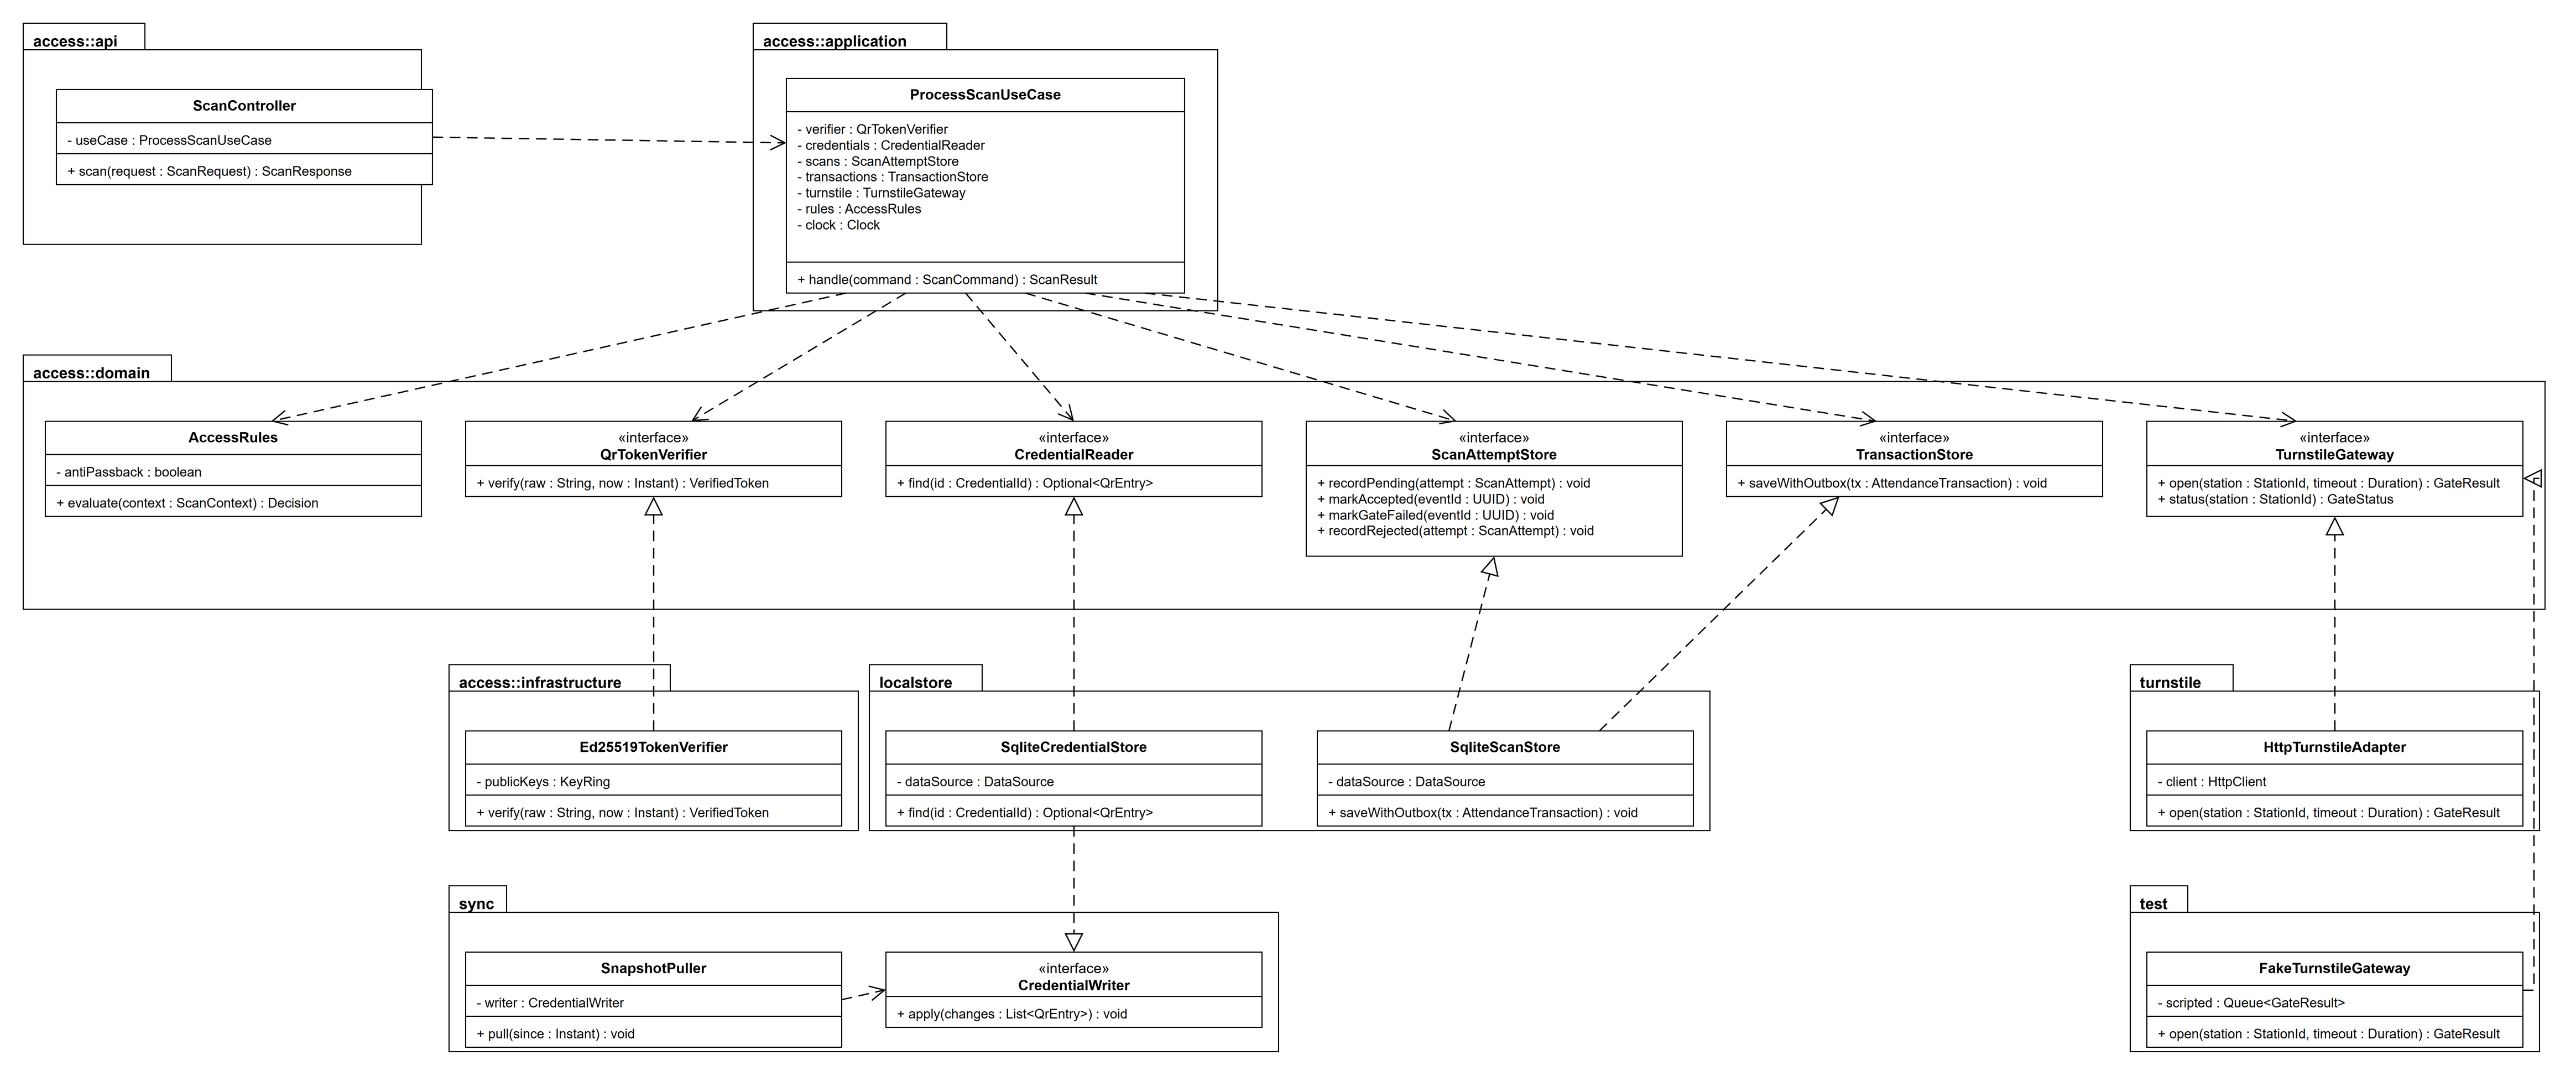
\includegraphics[width=0.92\textheight,height=0.92\textwidth,keepaspectratio]{figures/08_design_principles/class_access_ports.png}}
\caption{Lược đồ lớp các port và adapter của package \texttt{access}}
\label{fig:class-access}
\end{figure}

\subsubsection{Single Responsibility Principle}\label{sec:solid-srp}
\begin{itemize}
    \item \textit{Phát biểu:} Mỗi module, mỗi lớp chỉ có một lý do để thay đổi.
    \item \textit{Áp dụng:} ở mức component, G1, G2, G3 và G4 được tách riêng vì thay đổi vì những lý do khác nhau: quy tắc xác thực, nhà cung cấp cổng xoay, cách lưu trữ và giao thức đồng bộ. Ở mức lớp, \texttt{ProcessScanUseCase} chỉ điều phối luồng quét; quy tắc cho qua nằm trong \texttt{AccessRules}; việc kiểm tra chữ ký và thời hạn mã QR nằm trong \texttt{QrTokenVerifier}.
    \item \textit{Ví dụ:} khi đổi thuật toán ký mã QR, chỉ \texttt{Ed25519TokenVerifier} và adapter ký của C2 thay đổi; khi thêm quy tắc chống quẹt lặp chiều mới, chỉ \texttt{AccessRules} thay đổi.
    \item \textit{Lợi ích:} mỗi thay đổi chỉ cần kiểm thử lại một phạm vi nhỏ. \textit{Nguyên tắc liên quan:} DP-14.
\end{itemize}

\subsubsection{Open/Closed Principle}\label{sec:solid-ocp}
\begin{itemize}
    \item \textit{Phát biểu:} Phần mềm mở cho việc mở rộng nhưng đóng với việc sửa đổi.
    \item \textit{Áp dụng:} các điểm có khả năng thay đổi được đặt sau interface; hành vi mới được thêm bằng một cài đặt mới thay vì sửa mã đang chạy.
    \item \textit{Ví dụ:} thêm nhà cung cấp cổng xoay mới bằng một lớp mới cài đặt \texttt{TurnstileGateway} theo kiểu plugin của Gate Agent (ADR-04), cấu hình chọn adapter cho từng trạm; thêm định dạng xuất báo cáo bằng một lớp xuất báo cáo mới trong C6.
    \item \textit{Lợi ích:} mở rộng được mà không đụng tới mã nghiệp vụ đang chạy ổn định tại cổng. \textit{Nguyên tắc liên quan:} DP-16.
\end{itemize}

\subsubsection{Liskov Substitution Principle}\label{sec:solid-lsp}
\begin{itemize}
    \item \textit{Phát biểu:} Mọi cài đặt của một interface phải thay thế được cho nhau mà không làm sai hành vi của bên sử dụng.
    \item \textit{Áp dụng:} mỗi port có hợp đồng rõ ràng mà mọi cài đặt phải tuân theo. Ví dụ, mọi cài đặt \texttt{TurnstileGateway} phải trả về kết quả hoặc báo lỗi trong giới hạn thời gian chờ được truyền vào, không chặn luồng quét và không ném ngoại lệ ngoài hợp đồng.
    \item \textit{Ví dụ:} \texttt{FakeTurnstileGateway} được dùng thay cho \texttt{HttpTurnstileAdapter} khi kiểm thử các kịch bản cổng không phản hồi hoặc tải giờ giao ca mà không cần phần cứng; đồng hồ cố định (\texttt{java.time.Clock}) được dùng thay đồng hồ hệ thống để kiểm thử việc hết hạn của mã QR.
    \item \textit{Lợi ích:} \texttt{ProcessScanUseCase} được kiểm thử đầy đủ mà không cần thiết bị thật. \textit{Nguyên tắc liên quan:} DP-07, DP-16.
\end{itemize}

\subsubsection{Interface Segregation Principle}\label{sec:solid-isp}
\begin{itemize}
    \item \textit{Phát biểu:} Bên sử dụng không bị buộc phụ thuộc vào những thao tác mà nó không dùng.
    \item \textit{Áp dụng:} các port được thiết kế hẹp theo nhu cầu của từng bên sử dụng, kể cả khi cùng một lớp cài đặt nhiều port.
    \item \textit{Ví dụ:} \texttt{SqliteCredentialStore} cài đặt hai interface: \texttt{CredentialReader} chỉ có thao tác đọc, dành cho G1, và \texttt{CredentialWriter} chỉ có thao tác ghi, dành cho G4. Nhờ đó G1 không thể sửa bản sao credential (DP-04). Tương tự, \texttt{ScanAttemptStore} được tách khỏi \texttt{TransactionStore}; ở Central, interface tra cứu chấm công cho C6 được tách khỏi interface điều chỉnh chấm công của C4.
    \item \textit{Lợi ích:} mỗi bên chỉ thấy những thao tác được phép, phù hợp với nguyên tắc đặc quyền tối thiểu. \textit{Nguyên tắc liên quan:} DP-04, DP-10.
\end{itemize}

\subsubsection{Dependency Inversion Principle}\label{sec:solid-dip}
\begin{itemize}
    \item \textit{Phát biểu:} Module cấp cao không phụ thuộc module cấp thấp; cả hai phụ thuộc vào trừu tượng.
    \item \textit{Áp dụng:} các port được định nghĩa trong tầng \texttt{domain}; các adapter trong \texttt{infrastructure}, \texttt{localstore} và \texttt{turnstile} cài đặt chúng. \texttt{ProcessScanUseCase} chỉ phụ thuộc vào các interface; việc gắn cài đặt cụ thể được thực hiện bằng cơ chế tiêm phụ thuộc của Spring (ADR-10).
    \item \textit{Ví dụ:} trong Hình~\ref{fig:class-access}, mọi quan hệ realization đều hướng từ các package hạ tầng vào \texttt{access::domain}, không có quan hệ nào theo chiều ngược lại.
    \item \textit{Lợi ích:} thay đổi CSDL cục bộ, nhà cung cấp cổng xoay hay API của HR/Payroll không ảnh hưởng tới nghiệp vụ lõi (NFR-MOD-01). \textit{Nguyên tắc liên quan:} DP-16.
\end{itemize}

%==============================================================================
\subsection{Kiểm tra việc tuân thủ nguyên tắc}\label{sec:dp-compliance}
Các nguyên tắc chỉ có giá trị khi được kiểm tra trong quá trình phát triển. Bảng~\ref{tab:dp-compliance} nêu cách kiểm tra từng nguyên tắc.

\begingroup
\small
\renewcommand{\arraystretch}{1.3}
\begin{longtable}{|>{\centering\arraybackslash}p{1.4cm}|>{\raggedright\arraybackslash}p{11.0cm}|>{\raggedright\arraybackslash}p{2.6cm}|}
\caption{Cách kiểm tra việc tuân thủ các nguyên tắc thiết kế}\label{tab:dp-compliance}\\
\hline
\textbf{Nguyên tắc} & \textbf{Cách kiểm tra} & \textbf{ADR liên quan} \\
\hline
\endfirsthead
\hline
\textbf{Nguyên tắc} & \textbf{Cách kiểm tra} & \textbf{ADR liên quan} \\
\hline
\endhead
\hline
\endfoot
\endlastfoot
DP-01 & Kiểm thử dừng Gate Agent ngay sau khi ghi lượt quét rồi khởi động lại; kiểm thử cổng xoay không phản hồi & ADR-03 \\
\hline
DP-02 & Tài khoản CSDL của ứng dụng chỉ có quyền thêm bản ghi trên bảng giao dịch và nhật ký kiểm toán; kiểm thử điều chỉnh chấm công giữ nguyên bản gốc & ADR-03, ADR-08 \\
\hline
DP-03 & Kiểm thử gửi cùng một lô sự kiện hai lần và gửi lại cùng một đợt truyền & ADR-05, ADR-06 \\
\hline
DP-04 & Kiểm thử kiến trúc: chỉ module sở hữu được truy cập lớp lưu trữ của dữ liệu tương ứng & ADR-04, ADR-07 \\
\hline
DP-05 & Kiểm thử kiến trúc: \texttt{gate-agent} không phụ thuộc \texttt{central}; kiểm thử ngắt kết nối WAN trong khi quét & ADR-01 \\
\hline
DP-06 & Review thiết kế: không có lời gọi đồng bộ qua mạng trong luồng quét; theo dõi số bản ghi chờ trong outbox & ADR-05 \\
\hline
DP-07 & Review mã: mọi client gọi ra ngoài phải đặt giới hạn thời gian chờ; kiểm thử với \texttt{FakeTurnstileGateway} trả về hết thời gian chờ & ADR-06 \\
\hline
DP-08 & Kiểm thử vượt ngưỡng mất kết nối ở cả chiều vào và chiều ra & ADR-01 \\
\hline
DP-09 & Kiểm tra endpoint health check và chỉ số vận hành trong kiểm thử triển khai & ADR-07 \\
\hline
DP-10 & Kiểm thử phân quyền theo vai trò và theo phạm vi dữ liệu & ADR-08 \\
\hline
DP-11 & Kiểm thử với mã QR sai chữ ký, hết hạn và đã sử dụng; kiểm thử Gate Agent không có chứng chỉ hợp lệ & ADR-02, ADR-08 \\
\hline
DP-12 & Review hợp đồng dữ liệu gửi sang HR/Payroll; kiểm tra log không chứa mật khẩu, token (NFR-PRI-03) & ADR-08 \\
\hline
DP-13 & Kiểm thử mỗi thao tác nhạy cảm tạo đúng một bản ghi nhật ký kiểm toán & ADR-08 \\
\hline
DP-14 -- DP-16 & Kiểm thử kiến trúc tự động bằng ArchUnit và cơ chế kiểm tra module của Spring Modulith trong CI & ADR-07, ADR-10 \\
\hline
DP-17 & Review mã: không có giá trị ngưỡng, giới hạn thời gian chờ hay lịch viết cứng trong mã & ADR-07 \\
\hline
\end{longtable}
\endgroup

    

\subsection{Hiện thực các chức năng cốt lõi và giao diện người dùng}\label{sec:core-function-implementation}

\subsubsection{Xác thực người dùng và phát hành mã QR động}

Người dùng đăng nhập qua \texttt{POST /auth/login} để nhận JWT RS256 lưu trong
\texttt{sessionStorage} (tự xóa khi đóng tab, không dùng refresh token để giảm diện tấn công). Khi
tải trang, giao diện gọi \texttt{GET /auth/me} kiểm tra hiệu lực phiên và vai trò. Nhân viên có vai
trò \texttt{EMPLOYEE} gọi \texttt{GET /portal/qr-token} (không truyền tham số định danh; máy chủ lấy
mã nhân viên trực tiếp từ JWT để ngăn xem hộ mã của người khác theo FR-03). Chuỗi mã QR có định dạng
\texttt{TMC1.<base64url\_payload>.<base64url\_signature>}, hiệu lực 60 giây (chấp nhận lệch đồng hồ
$\pm 30$ giây tại trạm), được đề nghị làm mới mỗi 30 giây và gắn header
\texttt{Cache-Control: no-store}.

Quản trị viên (\texttt{ADMIN}) tra cứu danh sách nhân viên qua \texttt{GET /employees} và thực hiện
cấp mới, cấp lại hoặc thu hồi credential qua \texttt{POST /employees/\{code\}/qr/issue} và
\texttt{POST /employees/\{code\}/qr/revoke}. Khi thu hồi thành công, Portal của nhân viên nhận mã
lỗi \texttt{409 CREDENTIAL\_REVOKED} ở lần làm mới tiếp theo, đồng thời các Gate Agent đang trực
tuyến sẽ cập nhật danh sách từ chối trong vòng tối đa 60 giây. Hình~\ref{fig:ui-login} và
Hình~\ref{fig:ui-portal-qr-states} minh họa kết quả chạy thực tế của màn hình đăng nhập và hai trạng
thái mã QR trên Portal nhân viên.

\begin{figure}[H]
    \centering
    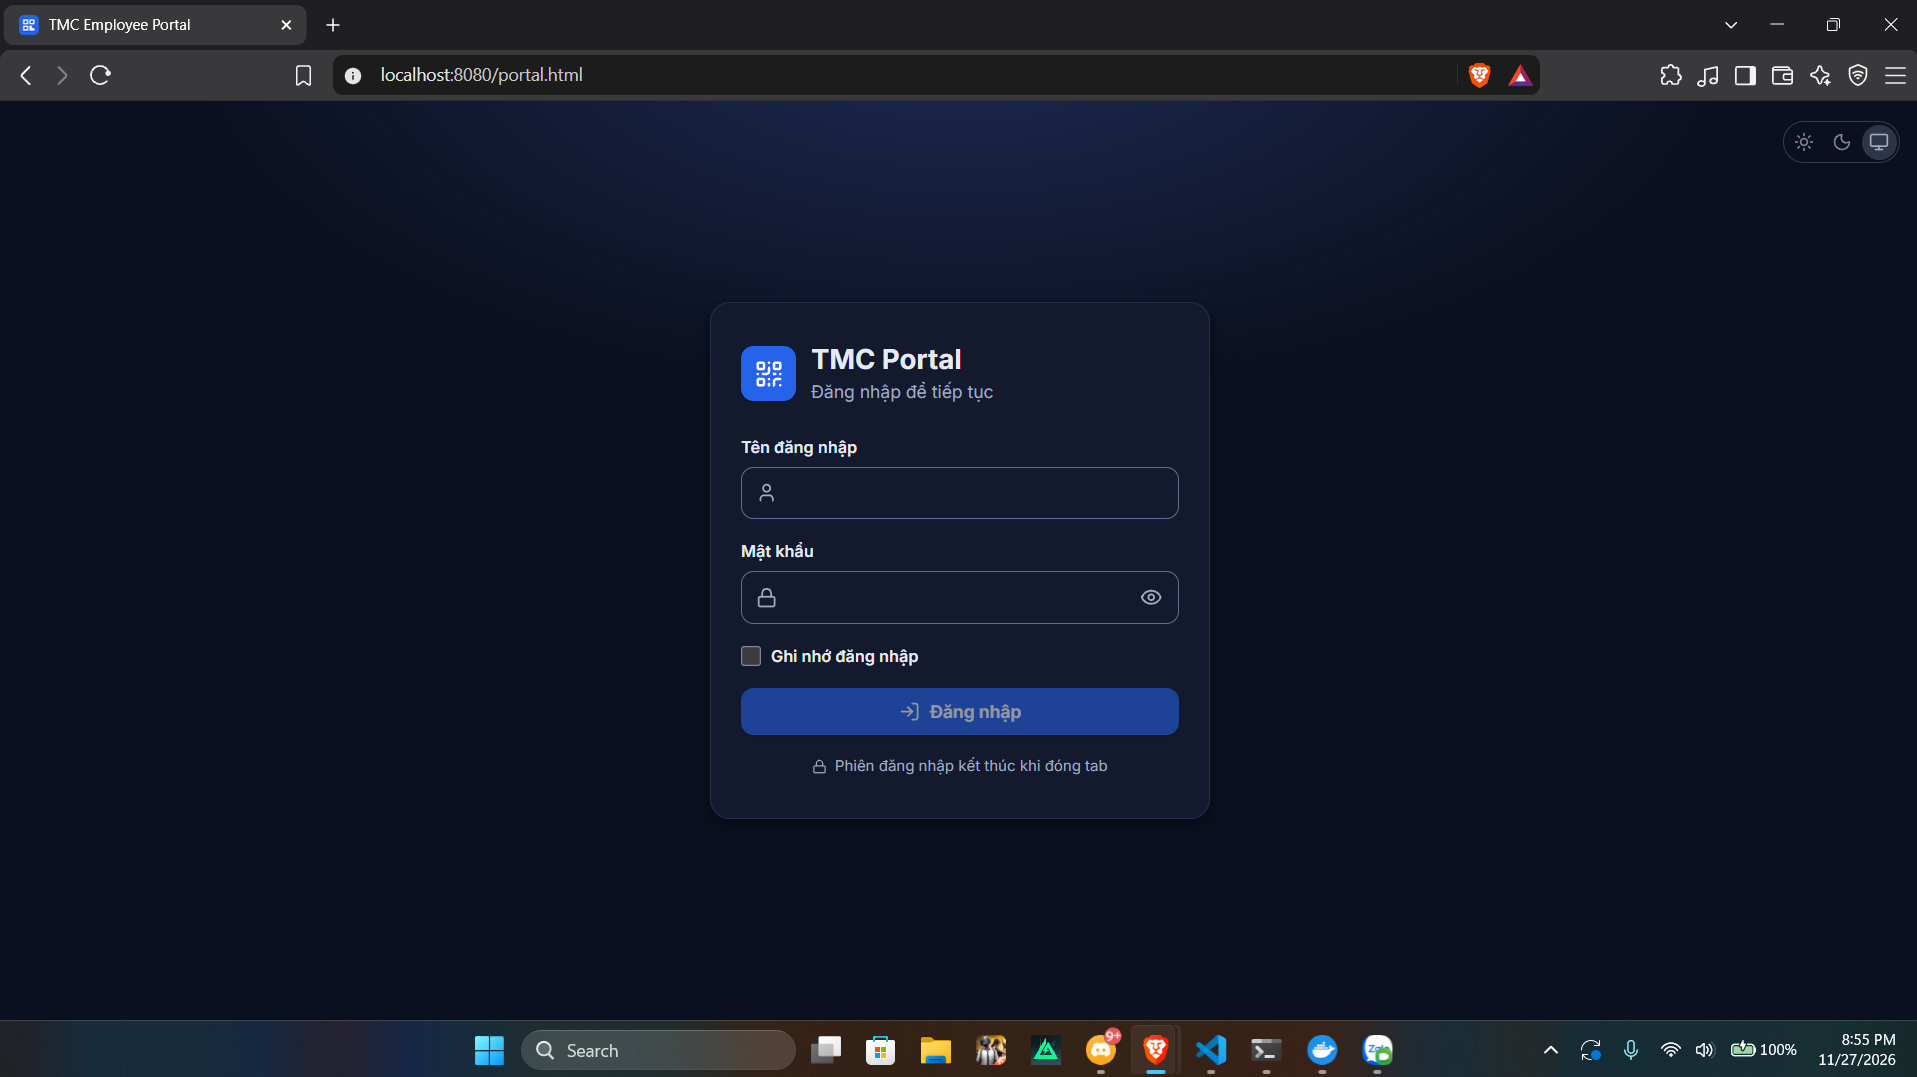
\includegraphics[width=0.82\textwidth]{figures/09_system_implementation/ui_login.png}
    \caption{Giao diện đăng nhập dùng chung cho Portal và Admin (\texttt{AU-01})}
    \label{fig:ui-login}
\end{figure}

\begin{figure}[H]
    \centering
    \begin{subfigure}[b]{0.49\textwidth}
        \centering
        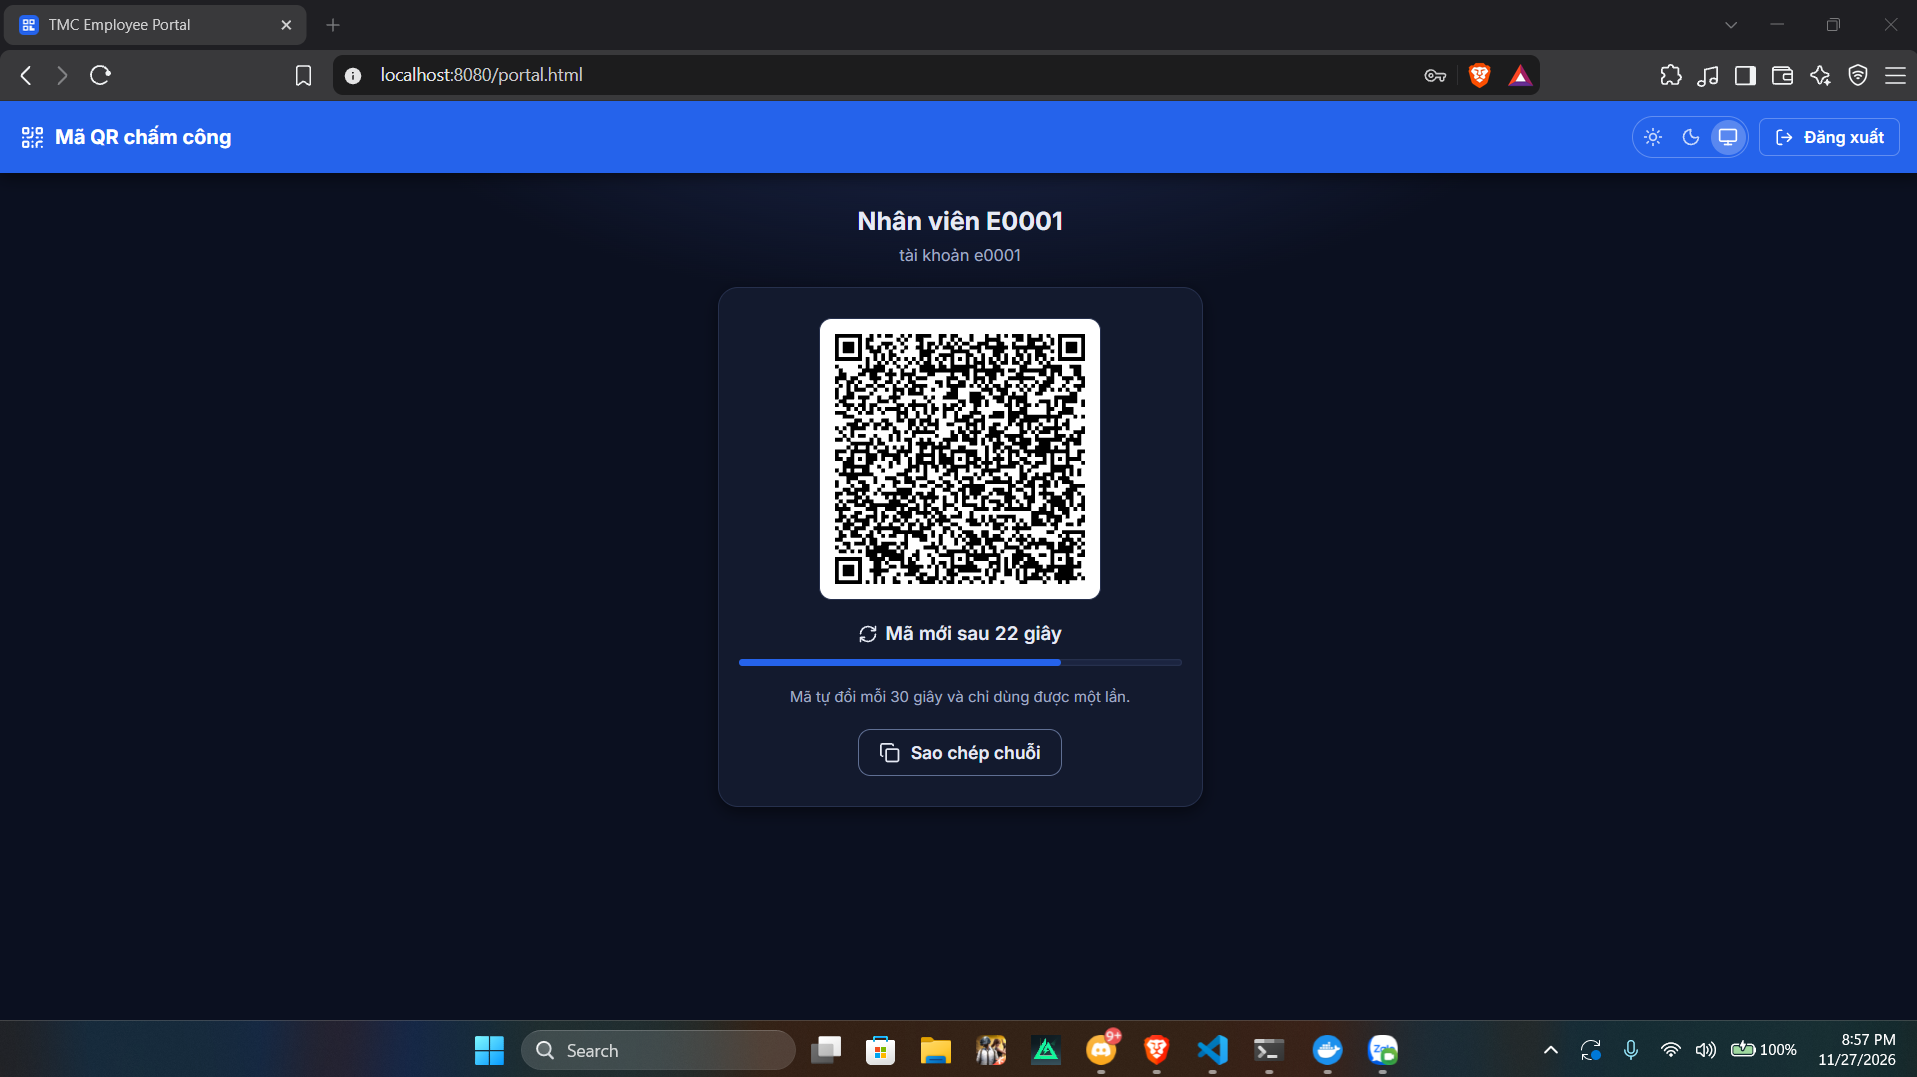
\includegraphics[width=\textwidth]{figures/09_system_implementation/ui_portal_qr.png}
        \caption{Mã QR động của nhân viên \texttt{E0001} (\texttt{P-01})}
        \label{fig:ui-portal-qr}
    \end{subfigure}
    \hfill
    \begin{subfigure}[b]{0.49\textwidth}
        \centering
        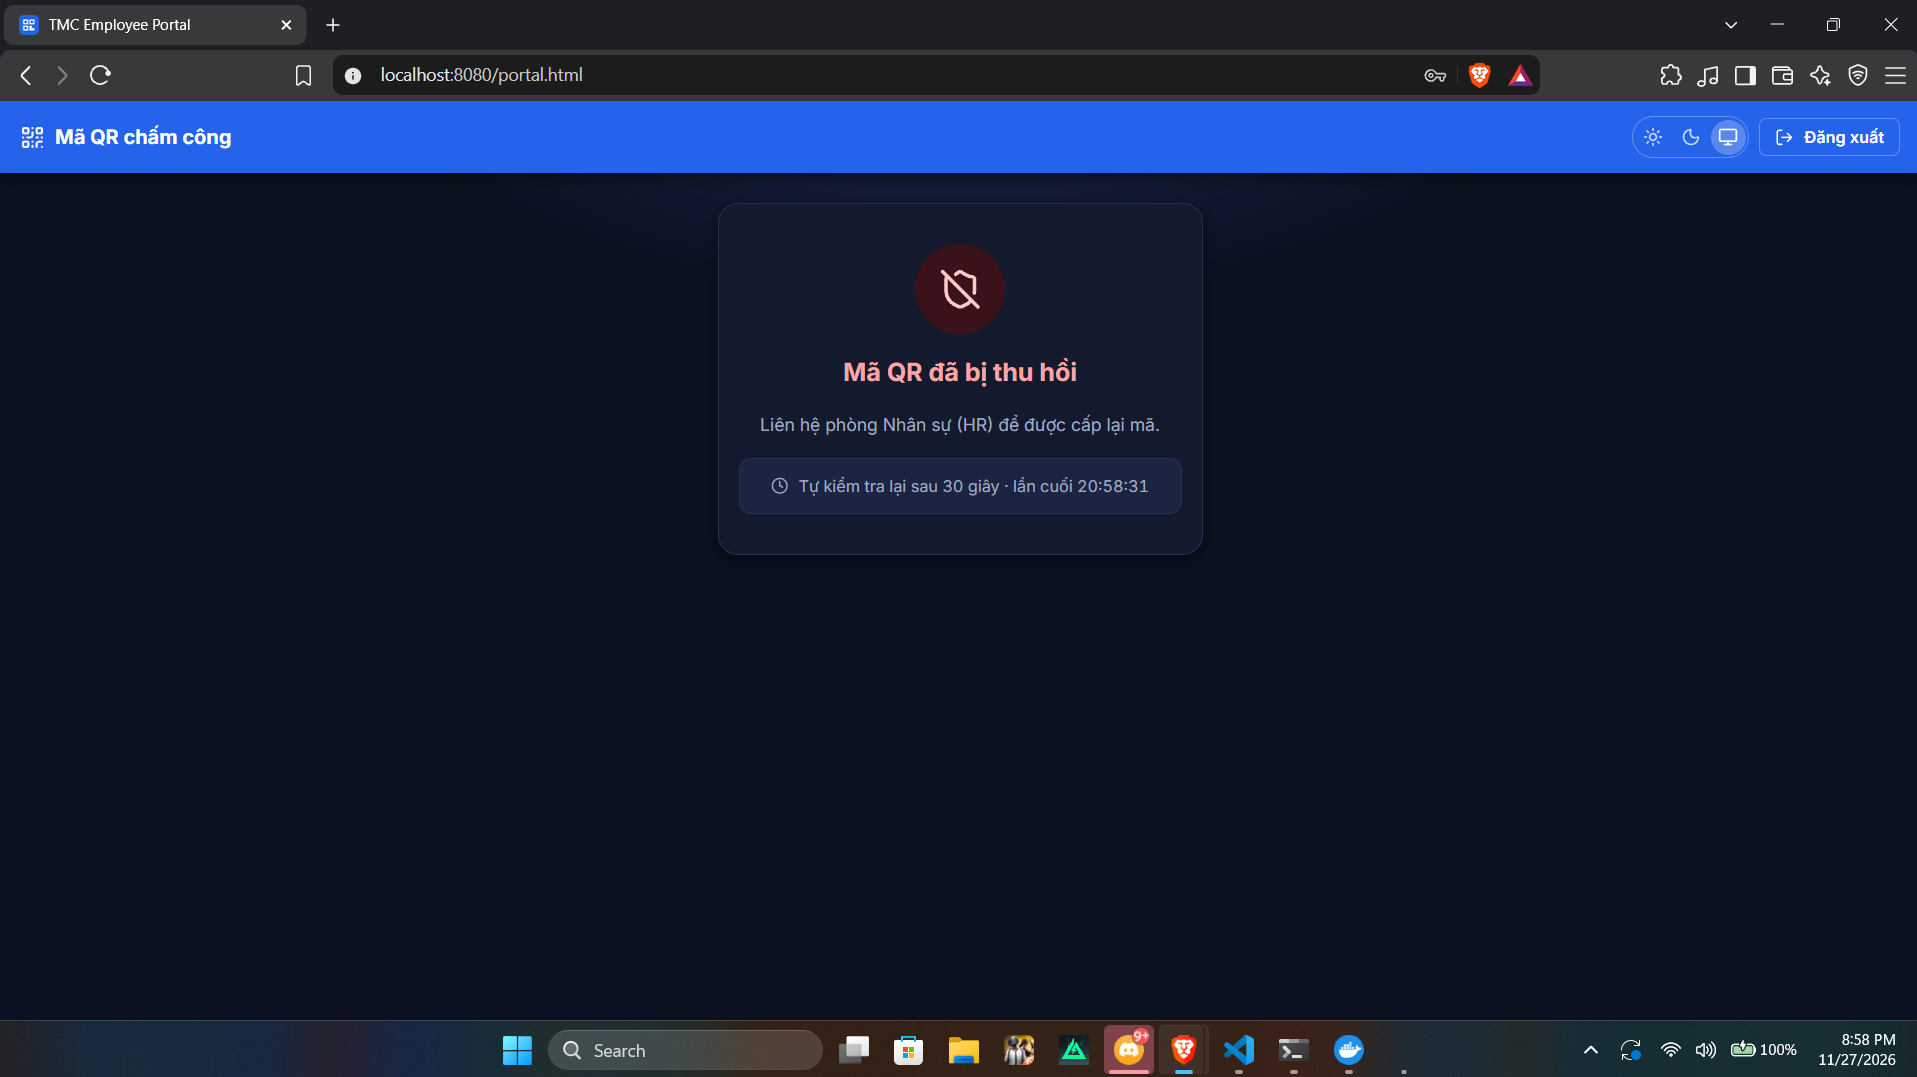
\includegraphics[width=\textwidth]{figures/09_system_implementation/ui_portal_revoked.png}
        \caption{Trạng thái mã QR đã bị thu hồi (\texttt{P-02})}
        \label{fig:ui-portal-revoked}
    \end{subfigure}
    \caption{Kết quả thực thi luồng cấp và thu hồi mã QR động trên Portal nhân viên}
    \label{fig:ui-portal-qr-states}
\end{figure}

\subsubsection{Xử lý lượt quét tại trạm cổng và phân loại kết quả}

Kiosk gửi mã trạm và chuỗi QR quét được tới \texttt{POST /scan} với timeout phía client là 2000 ms,
không tự động thử lại (vì nonce có thể đã bị tiêu thụ) và khóa nhập liệu trong khi đang chờ phản hồi
để tránh quét đúp. Điểm thiết kế quan trọng là mọi kết quả nghiệp vụ đều trả về mã HTTP 200 kèm
trường \texttt{result} thuộc một trong ba giá trị: \texttt{ACCEPTED} (màn hình xanh -- chỉ hiển thị
duy nhất cho trạng thái này theo NFR-AVL-03), \texttt{REJECTED} (màn hình đỏ kèm lý do cụ thể) hoặc
\texttt{GATE\_FAILED} (màn hình cam yêu cầu gặp bảo vệ). Bảng~\ref{tab:scan-reject-reasons} liệt kê
đầy đủ các mã kết quả, lý do từ chối và thông báo tiếng Việt chuẩn hóa giữa Gate Agent và Kiosk.

\small
\begin{longtable}{|>{\raggedright\arraybackslash}p{2.1cm}|>{\raggedright\arraybackslash}p{4.3cm}|>{\raggedright\arraybackslash}p{4.8cm}|>{\raggedright\arraybackslash}p{3.6cm}|}
\caption{Bảng mã kết quả quét, lý do từ chối và thông báo hiển thị trên Kiosk}\label{tab:scan-reject-reasons}\\
\hline
\textbf{Result} & \textbf{Mã \texttt{reason}} & \textbf{Ý nghĩa kỹ thuật} & \textbf{Thông báo Kiosk (Màu)} \\
\hline
\endfirsthead
\hline
\textbf{Result} & \textbf{Mã \texttt{reason}} & \textbf{Ý nghĩa kỹ thuật} & \textbf{Thông báo Kiosk (Màu)} \\
\hline
\endhead
\hline
\multicolumn{4}{r}{\textit{Còn tiếp sang trang sau...}} \\
\hline
\endfoot
\hline
\endlastfoot
\texttt{ACCEPTED} & \textit{(không có)} & Cổng xoay đã xác nhận mở và giao dịch chấm công đã được lưu cục bộ & Mời qua -- \{mã NV\} (VÀO/RA) \textit{(Xanh)} \\
\hline
\texttt{REJECTED} & \texttt{EXPIRED}, \texttt{NOT\_YET\_VALID} & Token ngoài cửa sổ hiệu lực 60 giây ($\pm 30$ giây lệch đồng hồ) & Mã QR đã hết hạn, vui lòng làm mới \textit{(Đỏ)} \\
\hline
\texttt{REJECTED} & \texttt{NONCE\_REUSED} & Token đã được sử dụng trước đó (chống chụp màn hình dùng lại) & Mã QR đã được sử dụng \textit{(Đỏ)} \\
\hline
\texttt{REJECTED} & \texttt{INVALID\_FORMAT}, \texttt{UNKNOWN\_KEY}, \texttt{BAD\_SIGNATURE} & Chuỗi không đúng định dạng \texttt{TMC1.}, khóa không tồn tại hoặc chữ ký sai & Mã QR không hợp lệ \textit{(Đỏ)} \\
\hline
\texttt{REJECTED} & \texttt{CREDENTIAL\_REVOKED}, \texttt{CREDENTIAL\_NOT\_FOUND} & Credential đã bị thu hồi hoặc chưa có trong bản sao cục bộ & Mã QR đã bị thu hồi hoặc không tồn tại \textit{(Đỏ)} \\
\hline
\texttt{REJECTED} & \texttt{EMPLOYEE\_INACTIVE} & Hồ sơ nhân viên không còn hoạt động & Nhân viên không còn hiệu lực \textit{(Đỏ)} \\
\hline
\texttt{REJECTED} & \texttt{UNKNOWN\_STATION}, \texttt{STATION\_DISABLED} & Trạm không thuộc Gate Agent này hoặc đang bị vô hiệu hóa (INV-03) & Trạm đang tạm ngừng \textit{(Đỏ)} \\
\hline
\texttt{REJECTED} & \texttt{ANTI\_PASSBACK} & Quét trùng chiều vào liên tiếp (vi phạm INV-04) & Bạn đã quét vào trước đó \textit{(Đỏ)} \\
\hline
\texttt{REJECTED} & \texttt{OFFLINE\_THRESHOLD\_EXCEEDED} & Cổng chiều vào bị từ chối do mất kết nối WAN vượt ngưỡng cho phép & Mất kết nối quá lâu -- vui lòng gặp bảo vệ \textit{(Đỏ)} \\
\hline
\texttt{GATE\_FAILED} & \texttt{GATE\_TIMEOUT}, \texttt{GATE\_ERROR}, \texttt{CIRCUIT\_OPEN} & Luật hợp lệ nhưng cổng xoay quá 800 ms, báo lỗi hoặc đang ngắt mạch 30 giây & Cổng chưa mở -- vui lòng gặp bảo vệ \textit{(Cam)} \\
\hline
\textit{Lỗi kết nối / HTTP 5xx} & \textit{(timeout client $> 2$ s)} & Không nhận được phản hồi xác định từ Gate Agent & Không xác định -- vui lòng gặp bảo vệ \textit{(Cam)} \\
\hline
\end{longtable}
\normalsize

Hình~\ref{fig:ui-kiosk-scan-results} minh họa hai kết quả thực thi thực tế tại trạm \texttt{BD-IN-01}:
lượt quét hợp lệ của nhân viên \texttt{E0001} được chấp nhận và mở cổng trong \textbf{0,37 giây}
(đáp ứng NFR-PER-01 $\leq 2$ giây), và lượt quét vào lặp lại ngay sau đó bị từ chối với lỗi chống
quét trùng làn (\texttt{ANTI\_PASSBACK}, INV-04) trong \textbf{0,01 giây}.

\begin{figure}[H]
    \centering
    \begin{subfigure}[b]{0.49\textwidth}
        \centering
        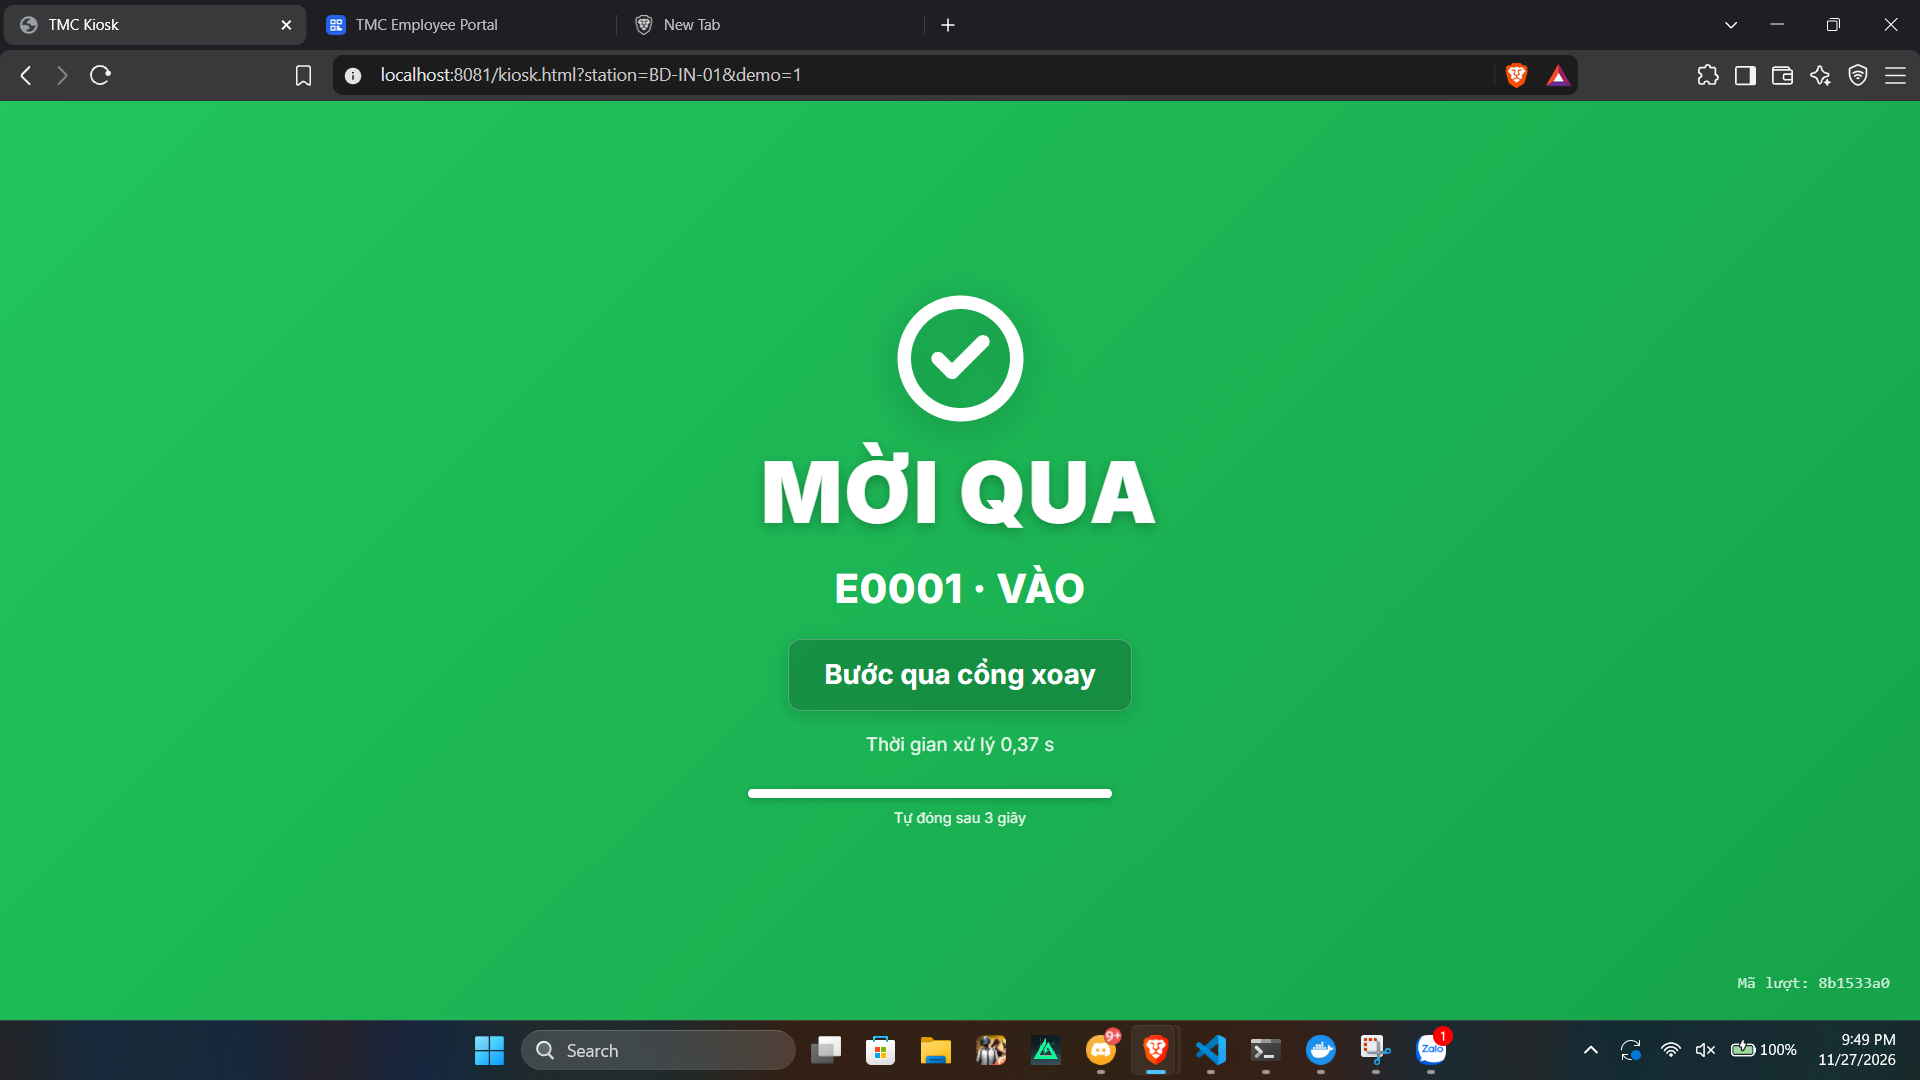
\includegraphics[width=\textwidth]{figures/09_system_implementation/ui_kiosk_accepted.png}
        \caption{Chấp nhận và mở cổng (\texttt{ACCEPTED}, 0,37 s)}
        \label{fig:ui-kiosk-accepted}
    \end{subfigure}
    \hfill
    \begin{subfigure}[b]{0.49\textwidth}
        \centering
        
\includegraphics[width=\textwidth]{figures/09_system_implementation/ui_kiosk_rejected.png}
        \caption{Từ chối trùng làn (\texttt{ANTI\_PASSBACK}, 0,01 s)}
        \label{fig:ui-kiosk-rejected}
    \end{subfigure}
    \caption{Kết quả hiển thị màn hình phủ \texttt{K-02} tại trạm cổng \texttt{BD-IN-01}}
    \label{fig:ui-kiosk-scan-results}
\end{figure}

\subsubsection{Lưu trữ cục bộ, hoạt động ngoại tuyến và giả lập cổng xoay}

Khi kết nối WAN tới Central bị gián đoạn (không có trao đổi thành công trong 30 giây), Gate Agent
chuyển sang trạng thái ngoại tuyến: mọi lượt quét tiếp tục được xác thực bằng dữ liệu tham chiếu
trong SQLite và lưu vào outbox để gửi bù khi có mạng. Nhằm cân bằng giữa tính sẵn sàng và bảo mật,
chiều \texttt{OUT} luôn tiếp tục hoạt động để không giữ nhân viên trong nhà máy, còn chiều
\texttt{IN} sẽ bị từ chối với lý do \texttt{OFFLINE\_THRESHOLD\_EXCEEDED} nếu thời gian mất kết nối
vượt ngưỡng cấu hình (mặc định 8 giờ trong vận hành và 2 phút trong cấu hình trình diễn). Kiosk định
kỳ gọi \texttt{GET /status} mỗi 3 giây để hiển thị biểu ngữ cảnh báo \textit{``OFFLINE -- \{n\} bản
ghi chờ đồng bộ''} và thông báo tạm ngừng chiều vào khi vượt ngưỡng.

Ở phía thiết bị, dịch vụ \texttt{turnstile-sim} mô phỏng chính xác API nhà cung cấp cổng xoay với
bốn chế độ điều khiển động qua \texttt{PUT /admin/behavior}:
\begin{itemize}
    \item \texttt{NORMAL}: mở cổng sau độ trễ ngẫu nhiên trong khoảng \texttt{latencyMs} (mặc định
    300--500 ms) và có thể phát sinh lỗi HTTP 500 theo xác suất \texttt{failureRate}.
    \item \texttt{TIMEOUT}: không mở cổng và trì hoãn 5 giây trước khi trả HTTP 504 (kích hoạt
    timeout 800 ms của Gate Agent).
    \item \texttt{ERROR}: không mở cổng và trả ngay HTTP 500 (\texttt{SIMULATED\_ERROR}).
    \item \texttt{EXECUTE\_THEN\_TIMEOUT}: vẫn thực thi mở cổng nhưng trì hoãn phản hồi 5 giây, dùng
    để kiểm chứng cơ chế truy vấn đối soát lệnh \texttt{GET /turnstiles/\{id\}/commands/\{requestId\}}
    của Gate Agent.
\end{itemize}

Hình~\ref{fig:ui-kiosk-outbox-sync} minh họa màn hình chờ quét làn vào (\texttt{K-01}) kết hợp bảng
điều khiển demo (\texttt{K-05}) khi Gate Agent đang đẩy bù các bản ghi còn tồn trong hàng đợi outbox
về Central sau khi khôi phục kết nối.

\begin{figure}[H]
    \centering
    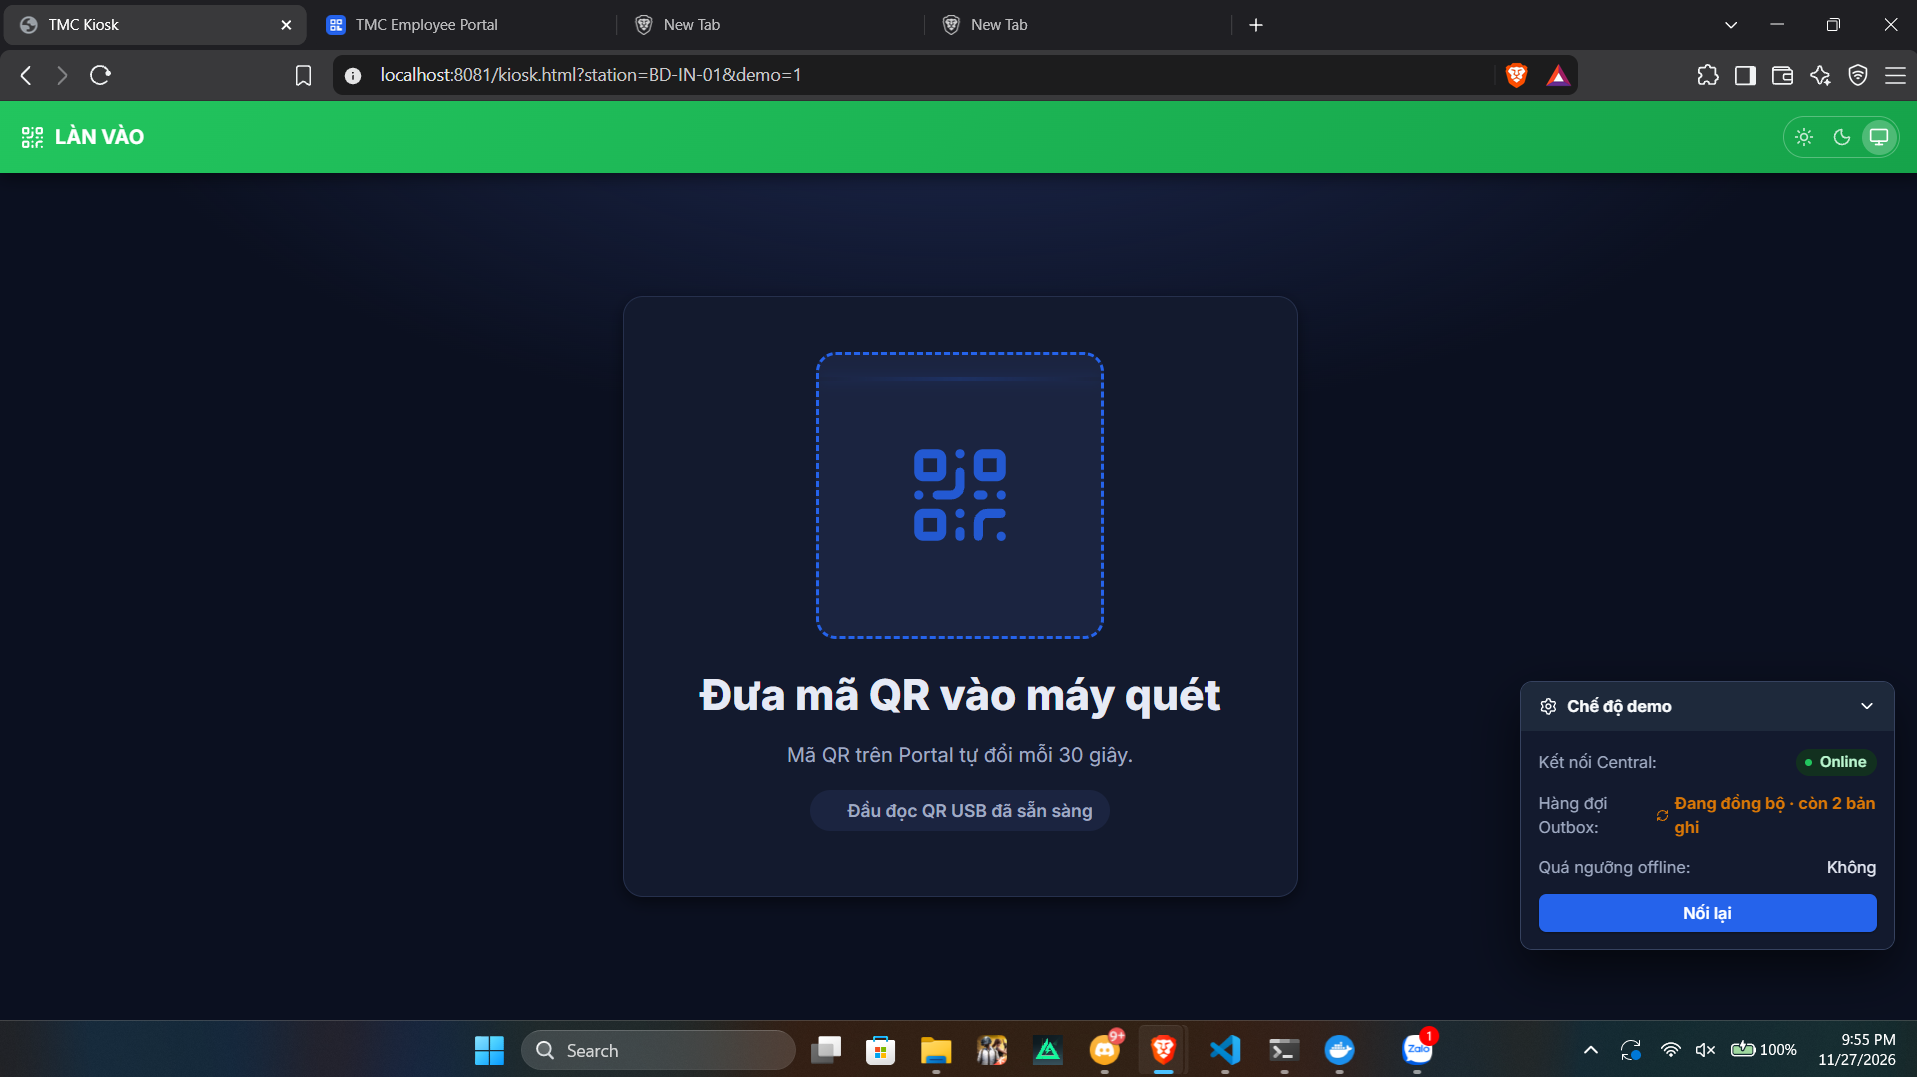
\includegraphics[width=0.82\textwidth]{figures/09_system_implementation/ui_kiosk_offline.png}
    \caption{Màn hình Kiosk làn vào (\texttt{K-01}) kèm bảng điều khiển demo (\texttt{K-05}) hiển thị hàng đợi outbox đang đồng bộ bù}
    \label{fig:ui-kiosk-outbox-sync}
\end{figure}

\subsubsection{Kiến trúc giao diện web và danh mục màn hình (Sitemap)}

Giao diện web được xây dựng bằng React và TypeScript, tách thành hai gói biên dịch độc lập: gói
\texttt{gate} (chỉ chứa trang \texttt{kiosk.html}, nhúng trực tiếp vào Gate Agent) và gói
\texttt{central} (chứa hai trang \texttt{portal.html} và \texttt{admin.html}, nhúng trực tiếp vào
Central). Cách đóng gói cùng nguồn gốc (same-origin) loại bỏ nhu cầu cấu hình CORS. Riêng trang
\texttt{admin.html} sử dụng định tuyến dạng hash (\texttt{\#/employees}, \texttt{\#/stations}) để
máy chủ tĩnh phục vụ trực tiếp mà không cần luật fallback SPA.

Về cấu trúc mã nguồn frontend, các thành phần được chia thành bốn lớp rõ ràng: lớp khởi tạo trang
(\texttt{entries}), lớp tính năng theo nghiệp vụ (\texttt{features/kiosk}, \texttt{features/portal},
\texttt{features/admin}, \texttt{features/auth}), lớp giao tiếp API dùng chung
(\texttt{shared/api/gateApi}, \texttt{shared/api/centralApi}, \texttt{shared/api/authSession} -- là
nơi duy nhất được phép gọi HTTP, sử dụng kiểu TypeScript sinh tự động từ OpenAPI 3.0.3) và lớp thành
phần hiển thị/hook dùng chung (\texttt{shared/ui}, \texttt{shared/hooks}).

Toàn bộ sitemap của phiên bản MVP gồm 14 màn hình, trạng thái và thành phần tương tác được đặc tả đầy
đủ trong Bảng~\ref{tab:web-sitemap-catalog}.

\small
\begin{longtable}{|>{\raggedright\arraybackslash}p{1.2cm}|>{\raggedright\arraybackslash}p{2.4cm}|>{\raggedright\arraybackslash}p{2.4cm}|>{\raggedright\arraybackslash}p{3.0cm}|>{\raggedright\arraybackslash}p{5.6cm}|}
\caption{Danh mục đầy đủ 14 màn hình và trạng thái giao diện web của MVP}\label{tab:web-sitemap-catalog}\\
\hline
\textbf{Mã} & \textbf{Tên màn hình} & \textbf{Trang / Loại} & \textbf{API sử dụng} & \textbf{Chức năng và hành vi chính} \\
\hline
\endfirsthead
\hline
\textbf{Mã} & \textbf{Tên màn hình} & \textbf{Trang / Loại} & \textbf{API sử dụng} & \textbf{Chức năng và hành vi chính} \\
\hline
\endhead
\hline
\multicolumn{5}{r}{\textit{Còn tiếp sang trang sau...}} \\
\hline
\endfoot
\hline
\endlastfoot
\texttt{K-01} & Chờ quét & \texttt{kiosk.html} \textit{(screen)} & \texttt{GET /status}, \texttt{POST /scan} & Màn hình chính tại trạm cổng (\texttt{?station=<id>}); giữ tiêu điểm (focus) trên ô nhập ẩn để nhận chuỗi từ máy quét USB; hiển thị biểu ngữ trạng thái mạng và độ sâu outbox mỗi 3 giây. \\
\hline
\texttt{K-02} & Kết quả quét & Phủ lên \texttt{K-01} \textit{(overlay)} & Kết quả \texttt{POST /scan} & Hiển thị nền xanh (\texttt{ACCEPTED}), đỏ (\texttt{REJECTED}) hoặc cam (\texttt{GATE\_FAILED}) kèm mã nhân viên, chiều vào/ra, thời gian xử lý (\texttt{elapsedMs}); tự đóng về \texttt{K-01} sau 3 giây. \\
\hline
\texttt{K-03} & Lỗi cấu hình trạm & \texttt{kiosk.html} \textit{(screen)} & \texttt{GET /status} & Hiển thị cho kỹ thuật viên khi thiếu tham số \texttt{station} hoặc mã trạm không thuộc danh sách trạm của Gate Agent. \\
\hline
\texttt{K-04} & Quét bằng webcam & \texttt{?camera=1} \textit{(mode)} & \texttt{POST /scan} & Bổ sung khung camera trực tiếp trên \texttt{K-01} để giải mã QR bằng webcam khi không có đầu đọc USB. \\
\hline
\texttt{K-05} & Bảng điều khiển demo & \texttt{?demo=1} \textit{(panel)} & \texttt{POST} \path{/admin/simulate-offline}, \texttt{GET /status} & Bảng bật/tắt giả lập mất kết nối WAN và theo dõi thông số outbox trực tiếp trên kiosk trong cấu hình demo. \\
\hline
\texttt{AU-01} & Đăng nhập & \texttt{portal.html}, \texttt{admin.html} \textit{(screen)} & \texttt{POST /auth/login}, \texttt{GET /auth/me} & Biểu mẫu nhập tài khoản/mật khẩu dùng chung cho Portal và Admin; khóa nút gửi khi đang xử lý; lưu JWT vào \texttt{sessionStorage}. \\
\hline
\texttt{AU-02} & Không có quyền truy cập & \texttt{portal.html}, \texttt{admin.html} \textit{(screen)} & \texttt{GET /auth/me} & Hiển thị khi tài khoản đã đăng nhập hợp lệ nhưng sai vai trò trang (ví dụ \texttt{ADMIN} mở Portal hoặc \texttt{EMPLOYEE} mở Admin), kèm nút đăng xuất. \\
\hline
\texttt{P-01} & Mã QR cá nhân & \texttt{portal.html} \textit{(screen)} & \texttt{GET} \path{/portal/qr-token} & Hiển thị mã QR động (mức sửa lỗi M) kèm đồng hồ đếm ngược 60 giây (tự động bù lệch đồng hồ máy chủ qua header \texttt{Date}); làm mới mỗi 30 giây và khi mở lại tab; có nút sao chép chuỗi QR. \\
\hline
\texttt{P-02} & Không có mã QR & \texttt{portal.html} \textit{(state)} & \texttt{GET} \path{/portal/qr-token} (409) & Thay thế \texttt{P-01} khi mã đã bị thu hồi, chưa được cấp hoặc nhân viên ngừng hoạt động; tự động hỏi lại mỗi 30 giây để hiển thị ngay khi HR cấp lại. \\
\hline
\texttt{A-01} & Khung trang quản trị & \texttt{admin.html} \textit{(layout)} & \texttt{GET /auth/me} & Thanh điều hướng chứa tên tài khoản, nút đăng xuất và hai tab chuyển đổi giữa \texttt{A-02} (\texttt{\#/employees}) và \texttt{A-04} (\texttt{\#/stations}). \\
\hline
\texttt{A-02} & Tab Nhân viên & \texttt{\#/employees} \textit{(tab)} & \texttt{GET /employees} & Bảng danh sách nhân viên kèm trạng thái credential; hỗ trợ lọc theo phòng ban, tìm kiếm theo mã/tên (debounce 300 ms), chọn từng dòng hoặc nhiều dòng. \\
\hline
\texttt{A-03} & Hộp thoại thao tác QR & Dialog trên \texttt{A-02} & \texttt{POST} \path{.../qr/revoke}, \texttt{POST} \path{.../qr/issue} & Xác nhận cấp lại hoặc thu hồi mã QR cho một nhân viên; bắt buộc nhập lý do (3--200 ký tự) khi thu hồi và cập nhật lại đúng dòng nhân viên sau khi hoàn tất. \\
\hline
\texttt{A-04} & Tab Trạm & \texttt{\#/stations} \textit{(tab)} & \texttt{GET /stations} & Theo dõi danh sách trạm cổng của hai nhà máy, làm mới mỗi 5 giây: trạng thái trực tuyến/ngoại tuyến, thời điểm heartbeat gần nhất, độ sâu outbox và trạng thái cổng xoay. \\
\hline
\texttt{A-05} & Hộp thoại thao tác hàng loạt & Dialog trên \texttt{A-02} & \texttt{POST} \path{.../qr/revoke}, \texttt{POST} \path{.../qr/issue} & Hỗ trợ thu hồi hoặc cấp lại mã QR cho nhiều nhân viên đã chọn bằng cách gọi tuần tự từng API, kiểm tra điều kiện trước khi chạy, yêu cầu nhập chuỗi xác nhận nếu thu hồi từ 5 người trở lên và dừng ngay khi gặp 401/403. \\
\hline
\end{longtable}
\normalsize

Quy tắc bảo vệ điều hướng (route guard) của Portal và Admin được thực thi nhất quán: khi mở trang,
nếu không có token trong \texttt{sessionStorage} hoặc \texttt{GET /auth/me} trả về 401 thì xóa phiên
và chuyển về \texttt{AU-01}; nếu trả về 200 nhưng vai trò không khớp trang thì chuyển sang
\texttt{AU-02}. Mọi thao tác bị từ chối 401 từ bất kỳ màn hình nào đều buộc đăng nhập lại. Riêng
Kiosk (\texttt{K-01}--\texttt{K-05}) hoạt động không cần đăng nhập trong mạng LAN cô lập của nhà máy
theo ADR-08. Hình~\ref{fig:ui-admin-employees} và Hình~\ref{fig:ui-admin-stations} minh họa giao diện
quản trị thực tế của hai tab Nhân viên và Trạm cổng.

\begin{figure}[H]
    \centering
    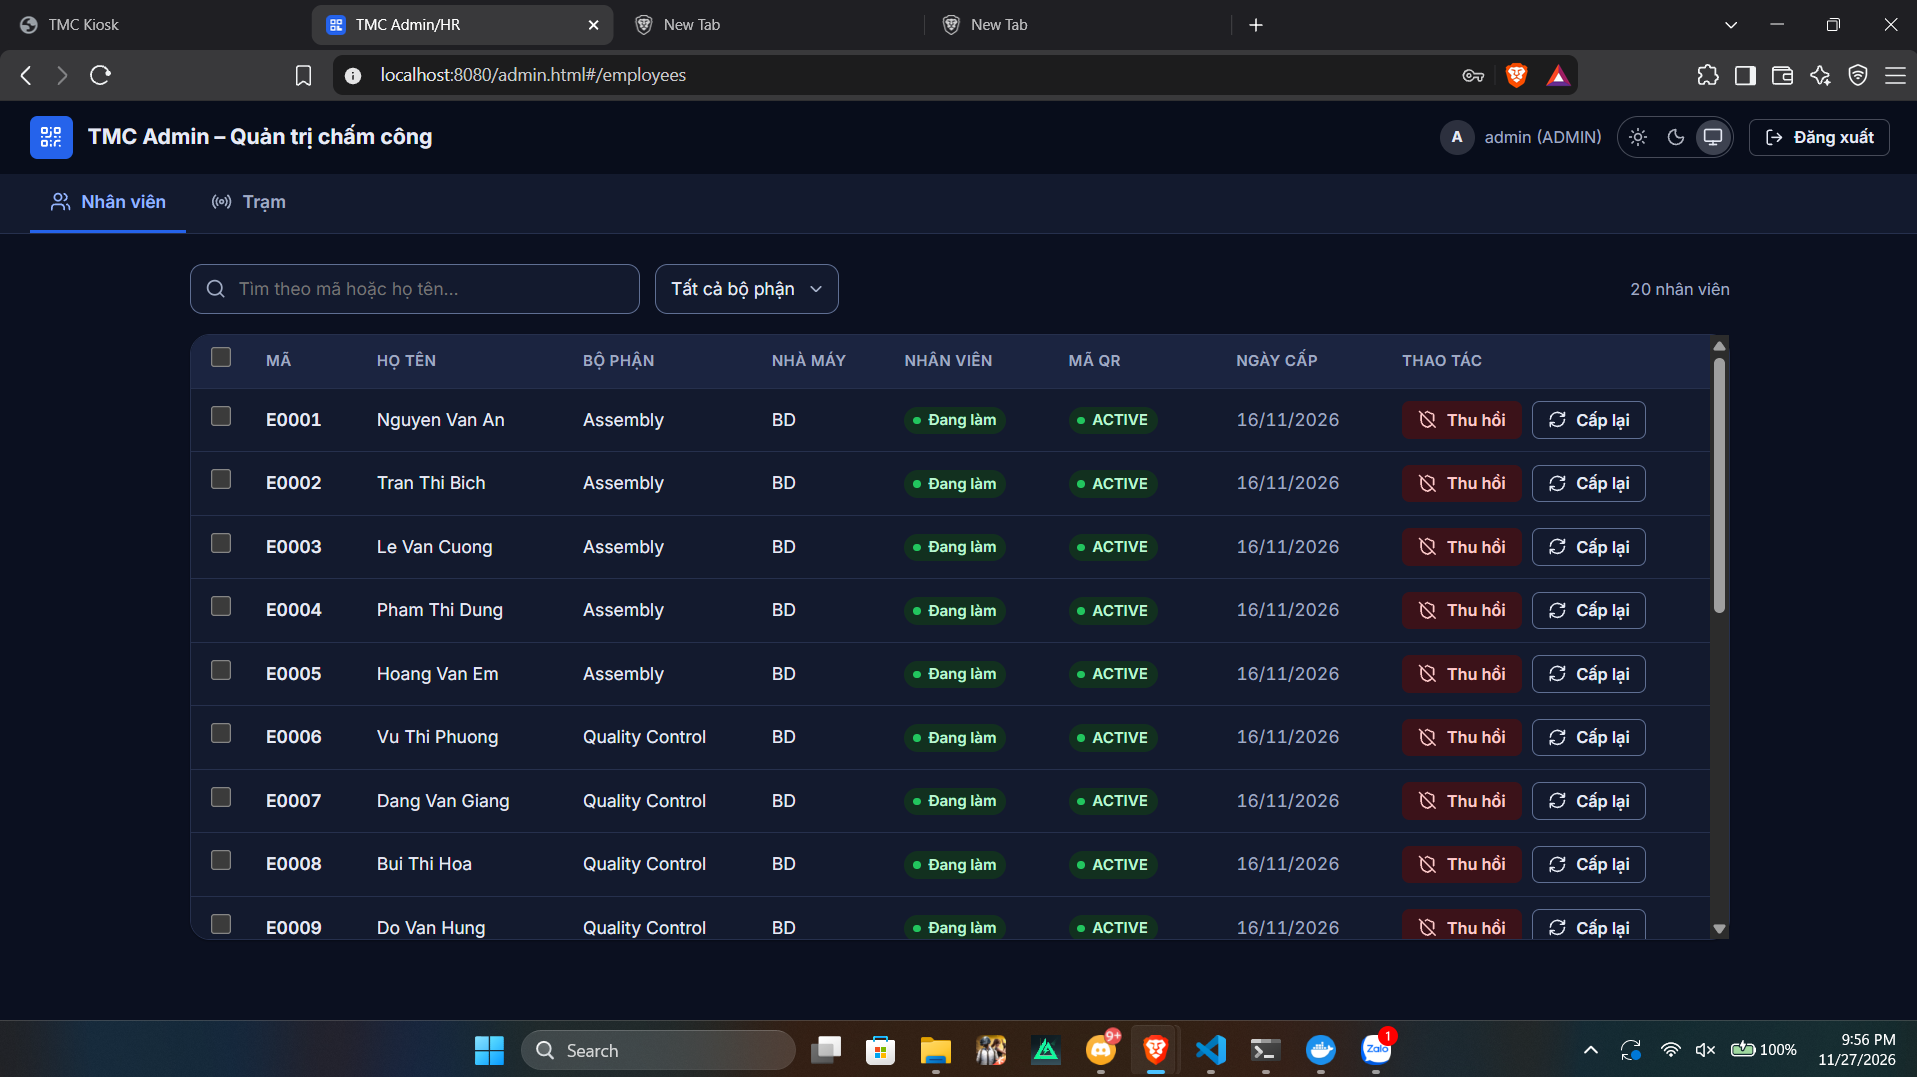
\includegraphics[width=0.88\textwidth]{figures/09_system_implementation/ui_admin_employees.png}
    \caption{Giao diện quản trị tab Nhân viên (\texttt{A-02}) hỗ trợ tìm kiếm, lọc bộ phận và thao tác cấp lại/thu hồi mã QR}
    \label{fig:ui-admin-employees}
\end{figure}

\begin{figure}[H]
    \centering
    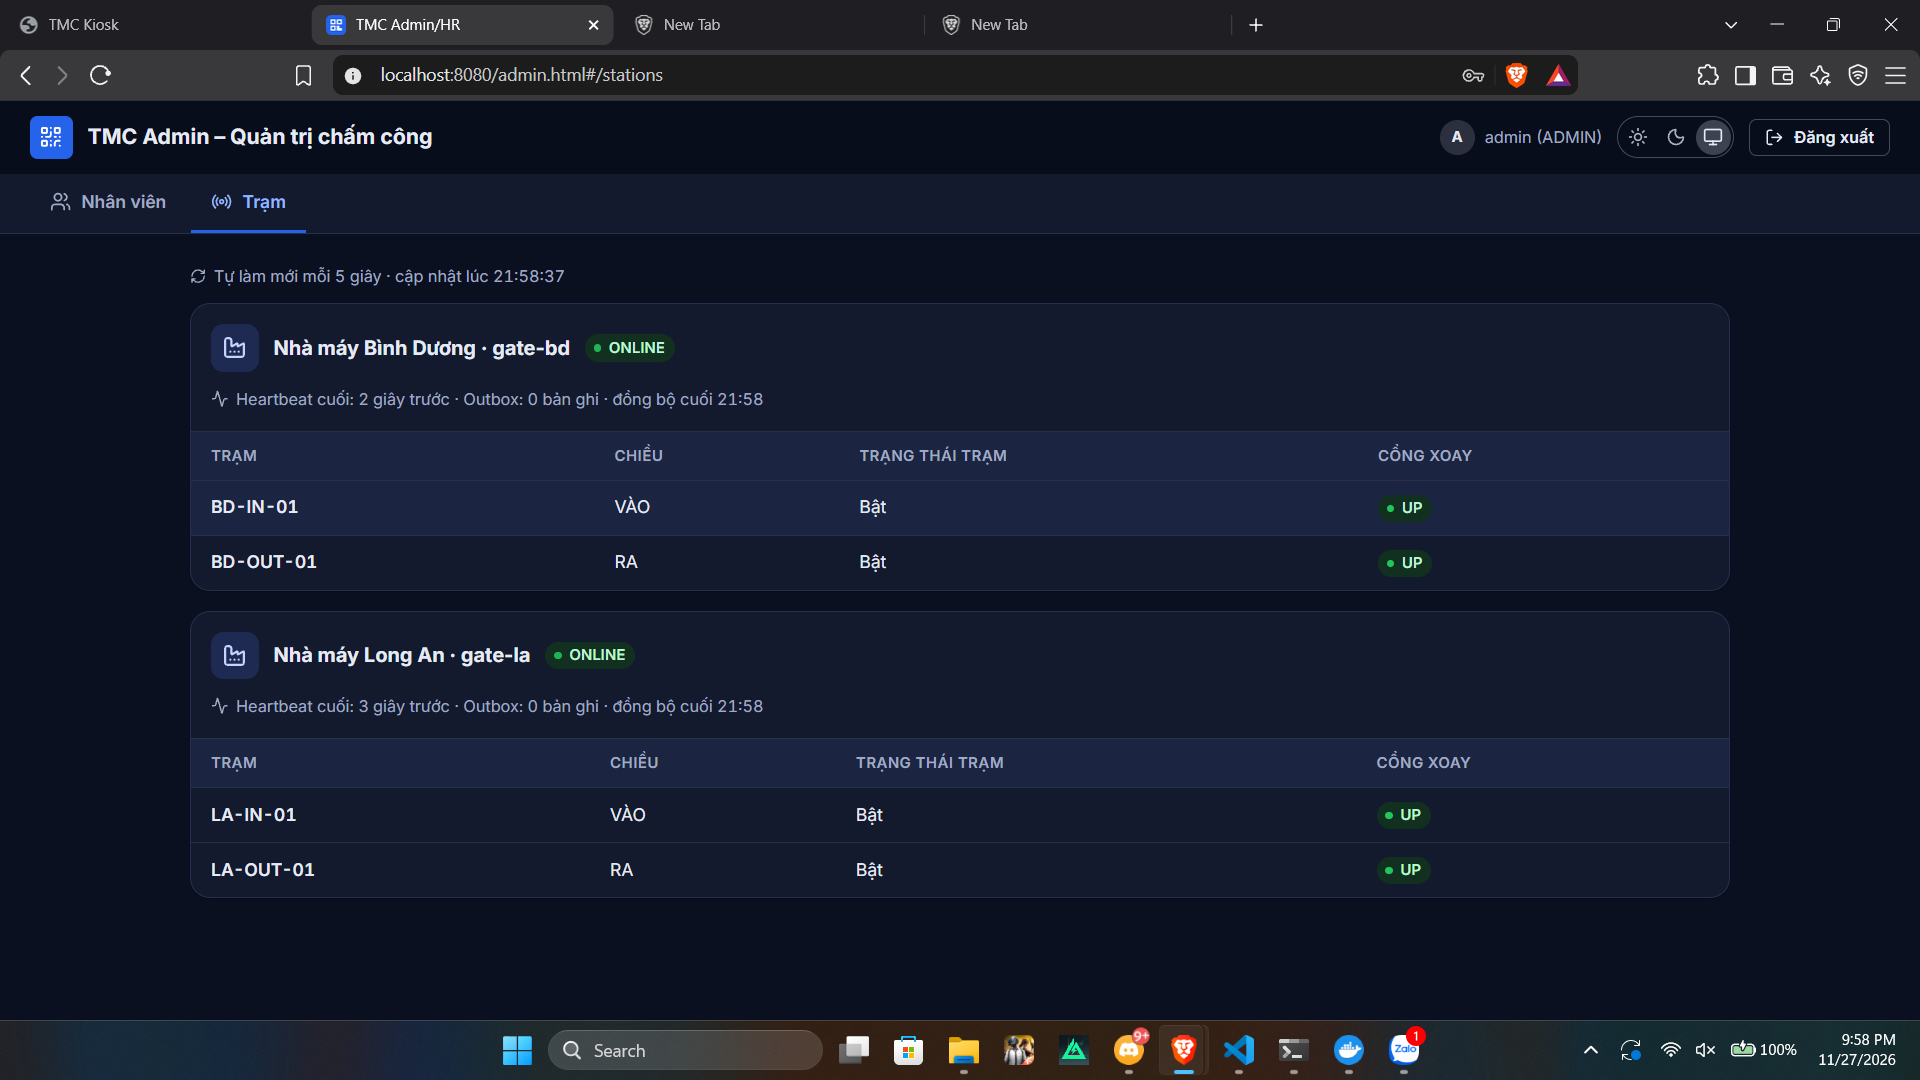
\includegraphics[width=0.88\textwidth]{figures/09_system_implementation/ui_admin_stations.png}
    \caption{Giao diện quản trị tab Trạm (\texttt{A-04}) giám sát trạng thái trực tuyến, heartbeat, outbox và cổng xoay của hai nhà máy}
    \label{fig:ui-admin-stations}
\end{figure}

\subsection{Thiết kế và đặc tả hợp đồng API}\label{sec:api-design-implementation}

\subsubsection{Phương pháp contract-first và quy ước chung}

Hệ thống áp dụng phương pháp thiết kế API theo hướng \textit{contract-first} bằng đặc tả OpenAPI
3.0.3, làm chuẩn thống nhất cho cả sinh mã kiểu TypeScript phía frontend, tạo dữ liệu giả lập MSW và
đối chiếu tài liệu runtime tại \texttt{/v3/api-docs} do Springdoc công bố. Các quy ước giao tiếp dùng
chung trên toàn bộ 19 đường dẫn (20 thao tác) gồm:
\begin{itemize}
    \item \textbf{Định dạng dữ liệu:} Request và response thành công dùng
    \texttt{application/json; charset=utf-8} với tên trường theo \texttt{camelCase}, giá trị enum
    theo \texttt{UPPER\_SNAKE\_CASE}, dấu thời gian theo chuẩn ISO-8601 UTC (hậu tố \texttt{Z}), mã
    sự kiện và credential theo UUID v4, mã nhân viên theo mẫu \texttt{E[0-9]\{4\}}, mã trạm theo mẫu
    \texttt{[A-Z]\{2\}-(IN|OUT)-[0-9]\{2\}}.
    \item \textbf{Tương thích ngược:} Các trường không có giá trị được lược bỏ thay vì trả
    \texttt{null}; cả client và server đều bỏ qua trường chưa biết để việc bổ sung trường tùy chọn
    không phá vỡ các phiên bản đang chạy.
    \item \textbf{Định dạng lỗi chuẩn:} Mọi lỗi giao thức trả về theo chuẩn RFC 9457 Problem Details
    (media type \path{application/problem+json}) gồm \texttt{type}, \texttt{title}, \texttt{status},
    \texttt{detail} và trường \texttt{code} ổn định để client rẽ nhánh xử lý (riêng mã
    \texttt{VALIDATION\_ERROR} kèm thêm mảng \texttt{errors: [\{field, message\}]}).
    \item \textbf{Bảo mật nhật ký:} Tuyệt đối không ghi chuỗi QR thô (\texttt{raw}), JWT, mật khẩu
    hay \texttt{X-Gate-Key} vào log ứng dụng; chỉ ghi \texttt{eventId}, \texttt{cid} và tên đăng nhập
    (NFR-PRI-03).
\end{itemize}

\subsubsection{Danh mục đầy đủ các endpoint}

Hợp đồng API được chia thành bốn nhóm tương ứng với từng ranh giới triển khai và đối tượng tiêu thụ:
\textbf{Gate Agent} (cổng \texttt{:8081}/\texttt{:8082}, phục vụ Kiosk và bảo vệ), \textbf{Central}
(cổng \texttt{:8080}, phục vụ Portal và Admin), \textbf{Sync} (cổng \texttt{:8080/sync}, kết nối giữa
hai quantum Q1--Q2) và \textbf{Turnstile Simulator} (cổng \texttt{:9001}/\texttt{:9002}, giả lập
thiết bị cổng xoay). Bảng~\ref{tab:mvp-api-index} liệt kê toàn bộ 19 path / 20 operation của MVP.

\small
\begin{longtable}{|>{\raggedright\arraybackslash}p{1.9cm}|>{\raggedright\arraybackslash}p{1.5cm}|>{\raggedright\arraybackslash}p{4.6cm}|>{\raggedright\arraybackslash}p{2.2cm}|>{\raggedright\arraybackslash}p{4.4cm}|}
\caption{Danh mục đầy đủ 19 đường dẫn (20 thao tác) API của phiên bản MVP}\label{tab:mvp-api-index}\\
\hline
\textbf{Nhóm} & \textbf{Method} & \textbf{Path} & \textbf{Xác thực} & \textbf{Chức năng} \\
\hline
\endfirsthead
\hline
\textbf{Nhóm} & \textbf{Method} & \textbf{Path} & \textbf{Xác thực} & \textbf{Chức năng} \\
\hline
\endhead
\hline
\multicolumn{5}{r}{\textit{Còn tiếp sang trang sau...}} \\
\hline
\endfoot
\hline
\endlastfoot
Gate Agent & POST & \path{/scan} & LAN (không) & Xác minh QR, ghi lượt quét và mở cổng xoay \\
\hline
Gate Agent & GET & \path{/status} & LAN (không) & Trạng thái kết nối, outbox và sức khỏe cổng \\
\hline
Gate Agent & GET & \path{/guard/pending} & LAN (không) & Danh sách lượt còn \texttt{PENDING} trước khi khởi động lại \\
\hline
Gate Agent & POST & \path{/admin/simulate-offline} & LAN (profile demo) & Bật/tắt giả lập mất kết nối WAN \\
\hline
Central & POST & \path{/auth/login} & Công khai & Xác thực tài khoản và phát hành JWT RS256 \\
\hline
Central & GET & \path{/auth/me} & JWT (mọi vai trò) & Trả về danh tính và vai trò phiên hiện tại \\
\hline
Central & GET & \path{/portal/qr-token} & JWT (\texttt{EMPLOYEE}) & Phát hành mã QR động (hiệu lực 60 giây) \\
\hline
Central & GET & \path{/employees} & JWT (\texttt{ADMIN}) & Tra cứu, lọc danh sách nhân viên và trạng thái QR \\
\hline
Central & POST & \path{/employees/{code}/qr/issue} & JWT (\texttt{ADMIN}) & Cấp mới hoặc cấp lại credential QR (INV-01) \\
\hline
Central & POST & \path{/employees/{code}/qr/revoke} & JWT (\texttt{ADMIN}) & Thu hồi credential QR đang hoạt động kèm lý do \\
\hline
Central & GET & \path{/stations} & JWT (\texttt{ADMIN}) & Danh sách trạm cổng, trạng thái online và outbox \\
\hline
Sync & POST & \path{/sync/events} & \texttt{X-Gate-Key} & Đẩy lô 1--200 sự kiện theo cơ chế idempotent \\
\hline
Sync & GET & \path{/sync/snapshot} & \texttt{X-Gate-Key} & Kéo delta dữ liệu tham chiếu từ \texttt{since} version \\
\hline
Sync & POST & \path{/sync/heartbeat} & \texttt{X-Gate-Key} & Báo cáo trạng thái sống và outbox của Gate Agent \\
\hline
Simulator & POST & \path{/turnstiles/{id}/open} & LAN (không) & Mở cổng một lần (idempotent theo \texttt{requestId}) \\
\hline
Simulator & GET & \path{/turnstiles/{id}/commands/{requestId}} & LAN (không) & Kiểm tra lệnh mở cổng đã thực thi hay chưa \\
\hline
Simulator & GET & \path{/turnstiles/{id}/status} & LAN (không) & Trạng thái và số lượt mở của một cổng xoay \\
\hline
Simulator & GET & \path{/turnstiles} & LAN (không) & Danh sách trạng thái mọi cổng xoay hiện có \\
\hline
Simulator & GET, PUT & \path{/admin/behavior} & LAN (không) & Đọc hoặc cập nhật độ trễ, tỉ lệ lỗi và chế độ giả lập \\
\hline
\end{longtable}
\normalsize

Hình~\ref{fig:api-swagger-central} minh họa tài liệu OpenAPI 3.0.3 do Springdoc tự động công bố tại
\texttt{/swagger-ui.html} trên ứng dụng Central, khớp đầy đủ 10 endpoint thuộc năm controller của hai
nhóm Central và Sync.

\begin{figure}[H]
    \centering
    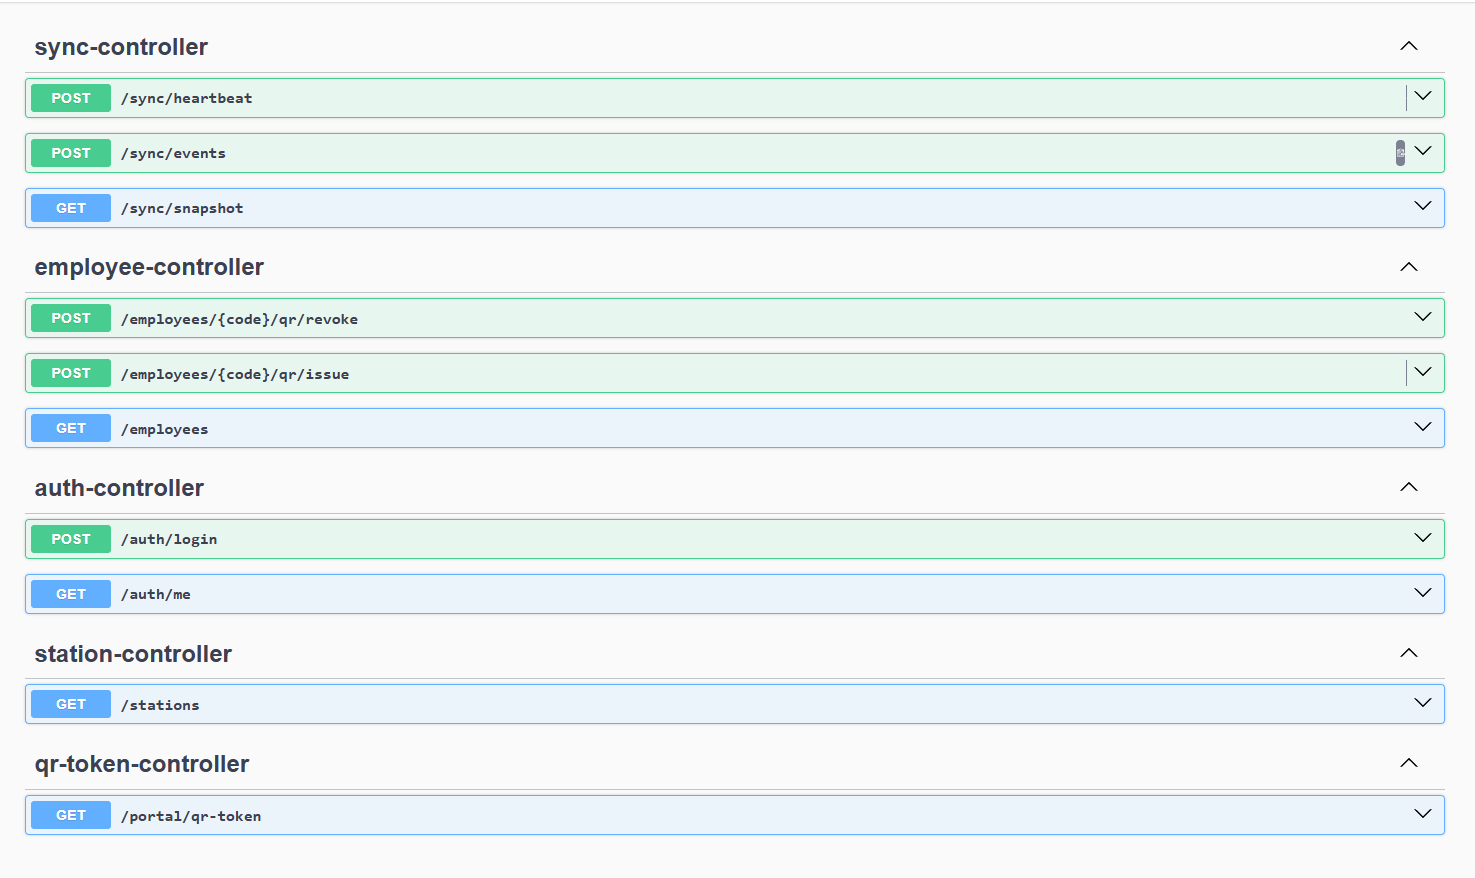
\includegraphics[width=0.92\textwidth]{figures/09_system_implementation/api_swagger_central.png}
    \caption{Giao diện Swagger UI công bố trực tiếp 10 endpoint Central và Sync từ hợp đồng OpenAPI 3.0.3}
    \label{fig:api-swagger-central}
\end{figure}

\subsubsection{Đặc tả chi tiết dữ liệu các API cốt lõi}

Bảng~\ref{tab:core-api-payloads} trình bày cấu trúc dữ liệu đầu vào (request) và đầu ra (response)
của các endpoint trọng yếu nhất trong bốn luồng hoạt động chính của hệ thống.

\small
\begin{longtable}{|>{\raggedright\arraybackslash}p{3.4cm}|>{\raggedright\arraybackslash}p{5.4cm}|>{\raggedright\arraybackslash}p{5.8cm}|}
\caption{Đặc tả dữ liệu đầu vào và đầu ra các API cốt lõi}\label{tab:core-api-payloads}\\
\hline
\textbf{Endpoint} & \textbf{Đầu vào (Request)} & \textbf{Đầu ra thành công (Response)} \\
\hline
\endfirsthead
\hline
\textbf{Endpoint} & \textbf{Đầu vào (Request)} & \textbf{Đầu ra thành công (Response)} \\
\hline
\endhead
\hline
\multicolumn{3}{r}{\textit{Còn tiếp sang trang sau...}} \\
\hline
\endfoot
\hline
\endlastfoot
\texttt{POST /scan} & JSON: \texttt{stationId} (chuỗi \texttt{BD-IN-01}), \texttt{raw} (1--1024 ký tự, chuỗi \texttt{TMC1.<payload>.<sig>}). & \texttt{200 OK}: \texttt{result} (\texttt{ACCEPTED} / \texttt{REJECTED} / \texttt{GATE\_FAILED}), \texttt{reason} (nếu không chấp nhận), \texttt{employeeCode} (chỉ có khi không bị \texttt{REJECTED}), \texttt{direction} (\texttt{IN}/\texttt{OUT}), \texttt{elapsedMs}, \texttt{eventId} (UUID). \\
\hline
\texttt{GET /status} & Không tham số. & \texttt{200 OK}: \texttt{gateId}, \texttt{online} (bool), \texttt{lastSyncAt}, \texttt{outboxDepth}, \texttt{offlineThresholdExceeded} (bool), \texttt{pendingReconcile}, \texttt{turnstiles} (bản đồ \texttt{stationId} $\rightarrow$ \texttt{UP}/\texttt{DOWN}/\texttt{CIRCUIT\_OPEN}). \\
\hline
\texttt{POST /auth/login} & JSON: \texttt{username} (1--32 ký tự, không phân biệt hoa thường), \texttt{password} (1--128 ký tự). & \texttt{200 OK}: \texttt{accessToken} (JWT RS256), \texttt{expiresAt} (+8 giờ), \texttt{role} (\texttt{EMPLOYEE}/\texttt{ADMIN}), \texttt{employeeCode} (chỉ có với \texttt{EMPLOYEE}). \\
\hline
\texttt{GET} \path{/portal/qr-token} & Header \texttt{Authorization: Bearer <JWT>}. Không có tham số. & \texttt{200 OK} (kèm \texttt{Cache-Control: no-store}): \texttt{raw} ($\approx 250$ ký tự), \texttt{expiresAt} (+60 giây), \texttt{refreshAfterSec} (\texttt{30}). \\
\hline
\texttt{POST} \path{/employees/{code}/qr/revoke} & Path \texttt{code} (\texttt{E0012}); JSON: \texttt{reason} (3--200 ký tự sau khi cắt khoảng trắng). & \texttt{200 OK}: đối tượng \texttt{EmployeeView} mới nhất (\texttt{code}, \texttt{fullName}, \texttt{departmentId}, \texttt{departmentName}, \texttt{factoryId}, \texttt{active}, \texttt{credentialId}, \texttt{credentialStatus=REVOKED}, \texttt{issuedAt}). \\
\hline
\texttt{POST /sync/events} & Header \texttt{X-Gate-Key}; JSON \texttt{EventBatch}: \texttt{contractVersion=1}, \texttt{gateId}, \texttt{factoryId}, \texttt{events} (1--200 \texttt{EventEnvelope} gồm \texttt{eventId}, \texttt{type} \texttt{SCAN\_ATTEMPT\_RECORDED} hoặc \texttt{ATTENDANCE\_RECORDED}, \texttt{occurredAt}, \texttt{payload}). & \texttt{200 OK} (\texttt{BatchAck}): \texttt{accepted} (mảng UUID mới lưu), \texttt{duplicates} (mảng UUID đã tồn tại), \texttt{rejected} (mảng \texttt{\{eventId, reason\}} với các lý do \texttt{INVALID\_PAYLOAD}, \texttt{UNKNOWN\_EVENT\_TYPE}, \texttt{UNKNOWN\_STATION}, \texttt{STATION\_NOT\_IN\_FACTORY}). \\
\hline
\texttt{GET /sync/snapshot} & Header \texttt{X-Gate-Key}; Query \texttt{since} (int64, mặc định \texttt{0} lấy toàn phần). & \texttt{200 OK} (\texttt{SnapshotDelta}): \texttt{fromVersion}, \texttt{toVersion}, \texttt{credentials} (không chứa họ tên theo DP-12), \texttt{publicKeys} (Ed25519 SPKI base64), \texttt{stations}, \texttt{settings} (\texttt{offlineThresholdMinutes}). \\
\hline
\texttt{POST /sync/heartbeat} & Header \texttt{X-Gate-Key}; JSON \texttt{Heartbeat}: \texttt{gateId}, \texttt{sentAt}, \texttt{outboxDepth}, \texttt{lastSyncAt}, \texttt{turnstileStatus}. & \texttt{204 No Content}. Central xem Gate là ngoại tuyến nếu quá 30 giây không nhận được heartbeat mới. \\
\hline
\texttt{POST} \path{/turnstiles/{id}/open} & Path \texttt{id} (\texttt{TS-BD-IN-01}); JSON: \texttt{requestId} (UUID chính là \texttt{eventId}). & \texttt{200 OK}: \texttt{requestId}, \texttt{executed=true}, \texttt{duplicate} (bool -- \texttt{true} nếu lệnh đã chạy trước đó), \texttt{at} (thời điểm mở cổng). \\
\hline
\end{longtable}
\normalsize

\subsubsection{Ma trận phân quyền và danh mục mã lỗi chuẩn}

Quyền truy cập API luôn được thực thi tại backend (DP-10); việc ẩn nút trên giao diện chỉ nhằm mục
đích trải nghiệm người dùng. Bảng~\ref{tab:api-auth-matrix} và Bảng~\ref{tab:api-error-codes} tổng
hợp ma trận phân quyền trên Central và danh mục mã lỗi Problem Details dùng chung trên toàn hệ thống.

\begin{table}[H]
\centering
\caption{Ma trận xác thực và phân quyền API phía Central}
\label{tab:api-auth-matrix}
\small
\renewcommand{\arraystretch}{1.25}
\begin{tabularx}{\textwidth}{|>{\raggedright\arraybackslash}X|>{\centering\arraybackslash}p{1.8cm}|>{\centering\arraybackslash}p{2.1cm}|>{\centering\arraybackslash}p{1.8cm}|>{\centering\arraybackslash}p{2.2cm}|}
\hline
\textbf{Nhóm đường dẫn} & \textbf{Công khai} & \textbf{\texttt{EMPLOYEE}} & \textbf{\texttt{ADMIN}} & \textbf{\texttt{X-Gate-Key}} \\
\hline
\texttt{/auth/login}, trang tĩnh, \texttt{/actuator/health}, \texttt{/v3/api-docs} & Cho phép & Cho phép & Cho phép & -- \\
\hline
\texttt{/auth/me} & 401 & Cho phép & Cho phép & -- \\
\hline
\texttt{/portal/qr-token} & 401 & Cho phép & 403 & -- \\
\hline
\texttt{/employees/**}, \texttt{/stations} & 401 & 403 & Cho phép & -- \\
\hline
\texttt{/sync/**} & 401 & 401 & 401 & Cho phép \\
\hline
\end{tabularx}
\end{table}

\begin{table}[H]
\centering
\caption{Danh mục mã lỗi chuẩn (RFC 9457 Problem Details) trên các nhóm API}
\label{tab:api-error-codes}
\small
\renewcommand{\arraystretch}{1.2}
\begin{tabularx}{\textwidth}{|>{\raggedright\arraybackslash}p{4.3cm}|>{\centering\arraybackslash}p{1.2cm}|>{\raggedright\arraybackslash}p{3.0cm}|>{\raggedright\arraybackslash}X|}
\hline
\textbf{Mã \texttt{code}} & \textbf{HTTP} & \textbf{API phát sinh} & \textbf{Ngữ cảnh và xử lý phía client} \\
\hline
\texttt{VALIDATION\_ERROR} & 400 & Mọi API & Thiếu trường bắt buộc, sai kiểu hoặc vượt độ dài; trả kèm danh sách \texttt{errors} theo từng trường. \\
\hline
\texttt{INVALID\_CREDENTIALS} & 401 & \texttt{POST /auth/login} & Sai tài khoản, sai mật khẩu hoặc tài khoản bị khóa (trả cùng một mã lỗi để tránh dò tài khoản). \\
\hline
\texttt{UNAUTHENTICATED} & 401 & Central (JWT) & Thiếu token, token hết hạn hoặc sai chữ ký; client xóa token và quay về màn hình \texttt{AU-01}. \\
\hline
\texttt{FORBIDDEN} & 403 & Central (JWT) & Token hợp lệ nhưng sai vai trò; client hiển thị màn hình \texttt{AU-02}. \\
\hline
\texttt{EMPLOYEE\_NOT\_FOUND} & 404 & \path{/employees/{code}/qr/*} & Mã nhân viên không tồn tại; giao diện tải lại danh sách. \\
\hline
\texttt{CREDENTIAL\_REVOKED}, \texttt{NO\_ACTIVE\_CREDENTIAL}, \texttt{EMPLOYEE\_INACTIVE} & 409 & \path{/portal/qr-token}, \path{/qr/issue}, \path{/qr/revoke} & Xung đột trạng thái nghiệp vụ; Portal chuyển sang \texttt{P-02} và thông báo liên hệ HR. \\
\hline
\texttt{CONCURRENT\_UPDATE} & 409 & \texttt{POST} \path{.../qr/issue} & Hai quản trị viên thao tác đồng thời trên cùng nhân viên; yêu cầu tải lại và thử lại. \\
\hline
\texttt{LOCAL\_STORE\_ERROR} & 500 & Gate \texttt{/scan}, \path{/guard/pending} & Lỗi ghi/đọc SQLite cục bộ; Kiosk báo \textit{``Không xác định -- vui lòng gặp bảo vệ''}. \\
\hline
\texttt{INVALID\_GATE\_KEY}, \texttt{GATE\_MISMATCH}, \texttt{UNKNOWN\_GATE} & 401 / 403 & \texttt{/sync/**} & Sai khóa trạm, sai ánh xạ \texttt{gateId} hoặc trạm chưa đăng ký; Gate giữ nguyên outbox và ghi log lỗi cấu hình. \\
\hline
\texttt{UNSUPPORTED\_}\allowbreak\texttt{CONTRACT\_VERSION}, \texttt{BATCH\_TOO\_LARGE} & 400 & \texttt{POST /sync/events} & Lệch phiên bản hợp đồng (\texttt{$\neq 1$}) hoặc lô vượt quá 200 sự kiện. \\
\hline
\texttt{SIMULATED\_ERROR}, \texttt{SIMULATED\_TIMEOUT} & 500 / 504 & Simulator \texttt{/open} & Lỗi giả lập phần cứng; Gate Agent ánh xạ tương ứng thành \texttt{GATE\_ERROR} và \texttt{GATE\_TIMEOUT}. \\
\hline
\end{tabularx}
\end{table}

Các kịch bản kiểm thử đơn vị, kiểm thử hợp đồng API, kiểm thử tích hợp đầu-cuối (bao gồm kịch bản
mất kết nối WAN, đồng bộ bù outbox, timeout cổng xoay và thu hồi mã QR) cũng như đánh giá hiệu năng
chịu tải giờ giao ca cho toàn bộ các chức năng và endpoint đã hiện thực ở chương này sẽ được trình
bày chi tiết trong Chương 10.

    \cleardoublepage
    \nocite{martin2017clean,richards2025fundamentals,clements2010documenting,sommerville2015software,slidesCO3017}
    \printbibliography[heading=bibintoc,title={Tài liệu tham khảo}]
    \appendix
    \cleardoublepage
    \phantomsection
    
    \section*{Phụ lục}
\addcontentsline{toc}{section}{Phụ lục}
\section{Danh sách lược đồ use case}

\begin{figure}[H]
    \centering
    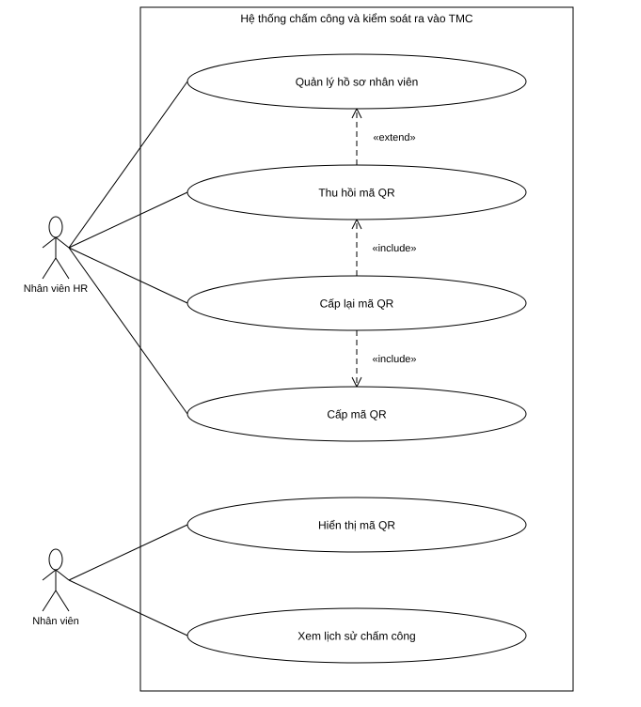
\includegraphics[width=\textwidth,height=0.72\textheight,keepaspectratio]{figures/appendix_use_case/uc_quan_ly_nguoi_dung_va_ma_qr.png}
    \caption{Sơ đồ use case nhóm Quản lý người dùng và mã QR}
    \label{fig:uc-quan-ly-nguoi-dung-ma-qr}
\end{figure}

\begin{figure}[H]
    \centering
    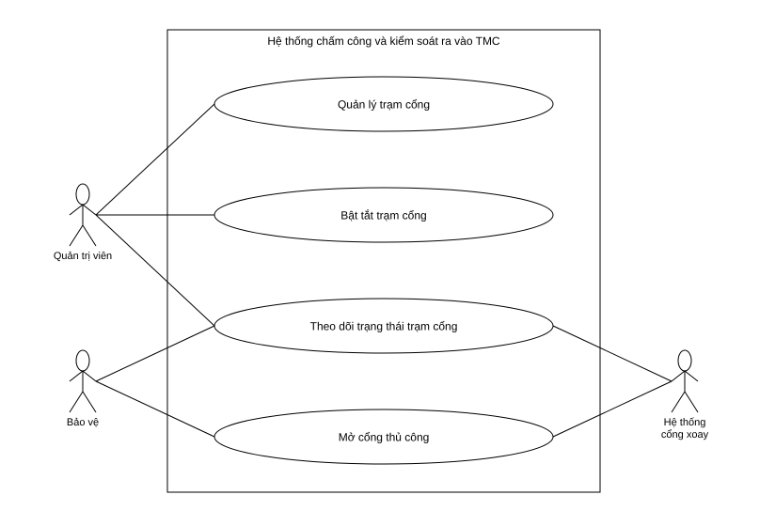
\includegraphics[width=\textwidth,height=0.72\textheight,keepaspectratio]{figures/appendix_use_case/uc_quan_ly_tram_cong.png}
    \caption{Sơ đồ use case nhóm Quản lý trạm cổng}
    \label{fig:uc-quan-ly-tram-cong}
\end{figure}

\begin{figure}[H]
    \centering
    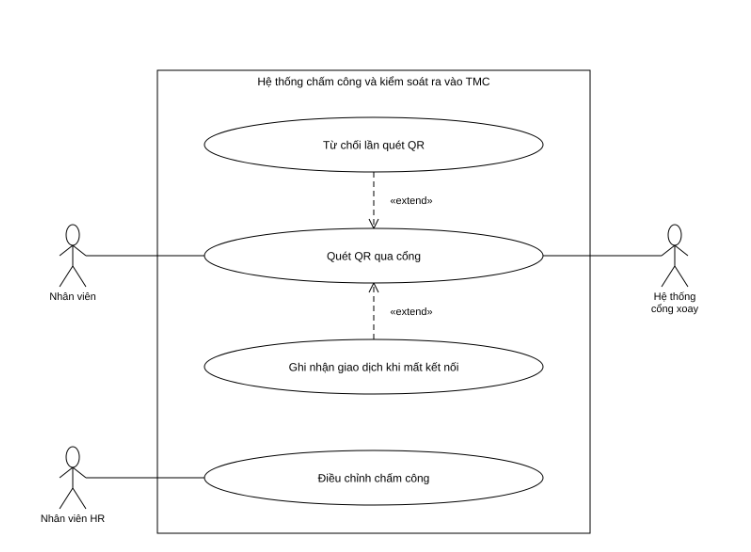
\includegraphics[width=\textwidth,height=0.72\textheight,keepaspectratio]{figures/appendix_use_case/uc_ghi_nhan_su_kien_cham_cong.png}
    \caption{Sơ đồ use case nhóm Ghi nhận sự kiện chấm công}
    \label{fig:uc-ghi-nhan-su-kien-cham-cong}
\end{figure}

\begin{figure}[H]
    \centering
    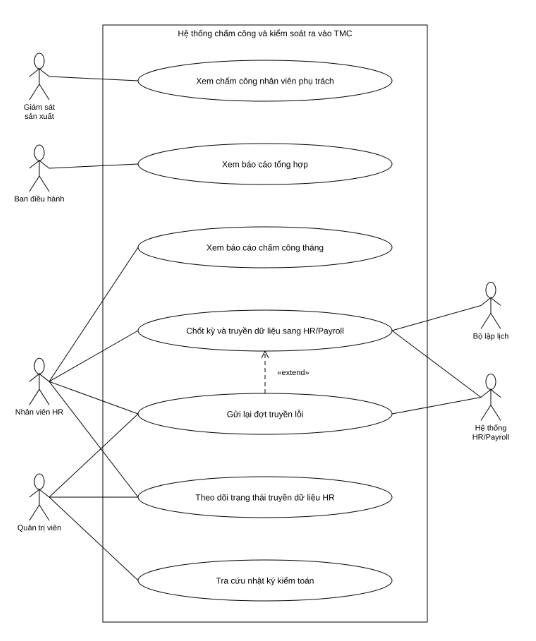
\includegraphics[width=\textwidth,height=0.72\textheight,keepaspectratio]{figures/appendix_use_case/uc_bao_cao_hr_payroll_kiem_toan.png}
    \caption{Sơ đồ use case nhóm Báo cáo, truyền dữ liệu HR/Payroll và kiểm toán}
    \label{fig:uc-bao-cao-hr-payroll-kiem-toan}
\end{figure}

\begin{figure}[H]
    \centering
    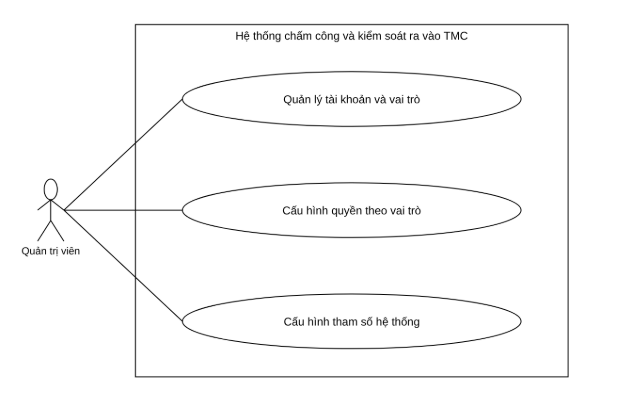
\includegraphics[width=\textwidth,height=0.72\textheight,keepaspectratio]{figures/appendix_use_case/uc_quan_tri_he_thong.png}
    \caption{Sơ đồ use case nhóm Quản trị hệ thống}
    \label{fig:uc-quan-tri-he-thong}
\end{figure}

\clearpage

\section{Use case quan trọng và đặc tả}

Nhóm chọn 4 use case có ý nghĩa kiến trúc trong số các use case ở phần thiết kế yêu cầu vì chúng gắn với các FR đánh dấu ASR. Bảng dưới đây liệt kê các use case được chọn và lý do lựa chọn; các phần tiếp theo đặc tả từng use case.

\small
\renewcommand{\arraystretch}{1.25}
\begin{longtable}{|>{\raggedright\arraybackslash}p{2.8cm}|>{\raggedright\arraybackslash}p{3.0cm}|>{\raggedright\arraybackslash}p{3.0cm}|>{\raggedright\arraybackslash}p{5.8cm}|}
\caption{Các use case có ý nghĩa kiến trúc} \\
\hline
\textbf{Use case} & \textbf{FR liên quan} & \textbf{Đặc tính kiến trúc} & \textbf{Lý do chọn} \\
\hline
\endfirsthead
\hline
\textbf{Use case} & \textbf{FR liên quan} & \textbf{Đặc tính kiến trúc} & \textbf{Lý do chọn} \\
\hline
\endhead
\hline
\multicolumn{4}{r}{\textit{Còn tiếp sang trang sau...}} \\
\hline
\endfoot
\hline
\endlastfoot
UC-01. Quét QR qua cổng & FR-08, FR-10, FR-11, FR-12, FR-13, FR-14, FR-15, FR-16, FR-17 & Performance, Availability, Data Integrity & Là luồng chính của hệ thống: phải xử lý nhanh, ghi nhận giao dịch chính xác và tiếp tục hoạt động khi mất kết nối. \\
\hline
UC-02. Thu hồi mã QR & FR-01, FR-02, FR-04, FR-05, FR-06, FR-23, FR-25 & Security, Availability & Hiệu lực thu hồi phải đến được các trạm cổng trong tối đa 60 giây (INV-02), nên ảnh hưởng cách phân phối dữ liệu QR xuống trạm. \\
\hline
UC-03. Điều chỉnh chấm công & FR-16, FR-18, FR-21, FR-22, FR-23, FR-25 & Data Integrity, Auditability & Giao dịch chấm công bất biến; điều chỉnh phải giữ bản gốc và để lại dấu vết (INV-06, INV-08). \\
\hline
UC-04. Chốt kỳ và truyền dữ liệu sang HR/Payroll & FR-21, FR-22, FR-23, FR-28 & Reliability, Interoperability & Dữ liệu phải có mặt ở HR/Payroll trước 12:00 ngày 1 (NFR-03); kỳ đã khóa chỉ nhận điều chỉnh qua đợt bổ sung (INV-09). \\
\end{longtable}
\normalsize

\subsection{UC-01. Quét QR qua cổng}

\noindent\textbf{Actor:} Nhân viên (chính); Hệ thống cổng xoay (phụ).

\noindent\textbf{Mô tả:} Nhân viên đưa mã QR vào máy quét tại trạm cổng để vào hoặc ra nhà máy. Hệ thống xác thực mã, mở cổng, ghi giao dịch chấm công và hiển thị kết quả trong $\leq 2$ giây (NFR-01).

\noindent\textbf{Điều kiện trước:}
\begin{itemize}
    \item Trạm cổng đang bật.
    \item Nhân viên có hồ sơ đang hoạt động và một mã QR đang hiệu lực.
\end{itemize}

\noindent\textbf{Điều kiện sau:}
\begin{itemize}
    \item Thành công: một giao dịch chấm công được lưu bền vững, cổng đã mở, kiosk hiển thị chấp nhận.
    \item Bị từ chối: không có giao dịch chấm công, lần quét bị từ chối được ghi nhận.
\end{itemize}

\noindent\textbf{Luồng chính:}
\begin{enumerate}
    \item Nhân viên đưa mã QR vào máy quét tại trạm cổng.
    \item Hệ thống kiểm tra mã hợp lệ, chưa bị thu hồi, nhân viên đang hoạt động và chiều vào/ra phù hợp với lần quét trước (FR-11).
    \item Hệ thống gửi lệnh mở cổng tới hệ thống cổng xoay qua API (FR-12).
    \item Hệ thống ghi giao dịch chấm công (mã nhân viên, thời điểm, trạm, chiều) và xác nhận đã lưu bền vững (FR-13).
    \item Kiosk hiển thị kết quả chấp nhận và nhân viên đi qua cổng (FR-14).
\end{enumerate}

\noindent\textbf{Luồng thay thế:}
\begin{description}
    \item[A1.] Mất kết nối với trung tâm (từ bước 2): trạm xác thực bằng danh sách mã QR hợp lệ đã nhân bản tại trạm, ghi giao dịch tại chỗ và mở cổng. Khi có kết nối, giao dịch được đồng bộ về trung tâm mà không tạo bản ghi trùng (FR-17).
    \item[A2.] Cổng hoặc hệ thống lỗi: bảo vệ mở cổng thủ công và nhập lý do (FR-10); lượt vào/ra này được HR bổ sung chấm công ở UC-03 theo FR-16.
\end{description}

\noindent\textbf{Ngoại lệ:}
\begin{description}
    \item[E1.] Mã không hợp lệ, đã thu hồi, nhân viên bị vô hiệu hóa, sai chiều vào/ra (anti-passback) hoặc trạm đang tắt: hệ thống không mở cổng, kiosk hiển thị từ chối kèm lý do và lần quét bị từ chối được ghi nhận (FR-08, FR-11, FR-14, FR-15).
    \item[E2.] Hệ thống cổng xoay không phản hồi hoặc báo lỗi: hệ thống không ghi giao dịch chấm công và kiosk báo lỗi để bảo vệ xử lý (FR-10, FR-12, FR-13).
    \item[E3.] Lưu giao dịch thất bại: kiosk không báo thành công; nếu cổng đã mở, sự cố được ghi nhận để đối soát và HR bổ sung chấm công nếu cần (FR-13, FR-16).
\end{description}

\noindent\textbf{FR liên quan:} FR-08, FR-10, FR-11, FR-12, FR-13, FR-14, FR-15, FR-16, FR-17.

\subsection{UC-02. Thu hồi mã QR}

\noindent\textbf{Actor:} Nhân viên HR.

\noindent\textbf{Mô tả:} Nhân viên HR thu hồi mã QR đang hiệu lực của một nhân viên (mất điện thoại, nghỉ việc). Mã đã thu hồi không còn mở được cổng.

\noindent\textbf{Điều kiện trước:}
\begin{itemize}
    \item HR đã đăng nhập và có quyền quản lý mã QR.
    \item Nhân viên có một mã QR đang hiệu lực.
\end{itemize}

\noindent\textbf{Điều kiện sau:}
\begin{itemize}
    \item Mã QR chuyển sang trạng thái đã thu hồi tại trung tâm.
    \item Danh sách mã hợp lệ tại các trạm được cập nhật, trễ tối đa 60 giây khi kết nối bình thường (INV-02).
    \item Thao tác được ghi nhật ký kiểm toán (FR-06, FR-23).
\end{itemize}

\noindent\textbf{Luồng chính:}
\begin{enumerate}
    \item HR tìm nhân viên, chọn thu hồi mã QR và chọn lý do (mất điện thoại, nghỉ việc).
    \item Hệ thống đánh dấu mã QR là đã thu hồi (FR-04).
    \item Hệ thống ghi nhật ký kiểm toán: người thực hiện, thời điểm, mã QR, lý do (FR-06, FR-23).
    \item Hệ thống nhân bản thay đổi xuống các trạm cổng (FR-05).
    \item Hệ thống thông báo thu hồi thành công cho HR.
\end{enumerate}

\noindent\textbf{Luồng thay thế:}
\begin{description}
    \item[A1.] Nhân viên nghỉ việc: HR vô hiệu hóa hồ sơ nhân viên; hệ thống tự thu hồi mọi mã QR đang hiệu lực rồi tiếp tục từ bước 3 (FR-01).
    \item[A2.] Mất điện thoại: sau bước 2, HR cấp lại mã QR mới cho nhân viên; chỉ mã mới có hiệu lực (FR-02, FR-04).
\end{description}

\noindent\textbf{Ngoại lệ:}
\begin{description}
    \item[E1.] Nhân viên không có mã đang hiệu lực: hệ thống báo không có mã để thu hồi và không thay đổi dữ liệu.
    \item[E2.] Trạm cổng đang mất kết nối: thay đổi được đồng bộ khi trạm có kết nối trở lại; trong thời gian đó trạm có thể còn chấp nhận mã đã thu hồi (FR-05; INV-02).
    \item[E3.] HR không có quyền: hệ thống từ chối thao tác (FR-25).
\end{description}

\noindent\textbf{FR liên quan:} FR-01, FR-02, FR-04, FR-05, FR-06, FR-23, FR-25.

\subsection{UC-03. Điều chỉnh chấm công}

\noindent\textbf{Actor:} Nhân viên HR.

\noindent\textbf{Mô tả:} Nhân viên HR bổ sung giao dịch chấm công bị thiếu hoặc điều chỉnh giao dịch sai (ví dụ do cổng lỗi), kèm lý do. Giao dịch gốc được giữ nguyên.

\noindent\textbf{Điều kiện trước:}
\begin{itemize}
    \item HR đã đăng nhập và có quyền điều chỉnh chấm công (FR-25).
    \item Dữ liệu cần điều chỉnh đã được xác định (giao dịch sai hoặc lượt vào/ra bị thiếu).
\end{itemize}

\noindent\textbf{Điều kiện sau:}
\begin{itemize}
    \item Một bản ghi điều chỉnh gồm lý do và người thực hiện được lưu; giao dịch gốc không bị sửa hoặc xóa (INV-06, INV-08).
    \item Thao tác được ghi nhật ký kiểm toán.
    \item Nếu kỳ đã khóa, điều chỉnh được chuyển vào đợt truyền bổ sung (INV-09).
\end{itemize}

\noindent\textbf{Luồng chính:}
\begin{enumerate}
    \item HR tra cứu chấm công của nhân viên theo ngày (FR-18).
    \item HR chọn bổ sung giao dịch thiếu hoặc điều chỉnh giao dịch sai và nhập lý do (FR-16).
    \item Hệ thống kiểm tra quyền và dữ liệu nhập (thời điểm, trạm, chiều vào/ra) (FR-16, FR-25).
    \item Hệ thống lưu bản ghi điều chỉnh tham chiếu giao dịch gốc (FR-16).
    \item Hệ thống ghi nhật ký kiểm toán và thông báo thành công (FR-23).
\end{enumerate}

\noindent\textbf{Luồng thay thế:}
\begin{description}
    \item[A1.] Giao dịch ghi nhầm: HR chọn hủy giao dịch kèm lý do; hệ thống tạo bản ghi điều chỉnh loại giao dịch đó khỏi báo cáo, không xóa dữ liệu gốc (FR-16).
    \item[A2.] Kỳ chấm công đã khóa: hệ thống vẫn nhận điều chỉnh và đưa vào đợt truyền bổ sung, không gửi lại đợt chính đã gửi thành công (FR-21, INV-09).
\end{description}

\noindent\textbf{Ngoại lệ:}
\begin{description}
    \item[E1.] HR không nhập lý do: hệ thống từ chối lưu và yêu cầu nhập lý do (FR-16).
    \item[E2.] Dữ liệu không hợp lệ (ví dụ thời điểm ở tương lai, trạm không tồn tại): hệ thống báo lỗi và không lưu (FR-16).
    \item[E3.] HR không có quyền: hệ thống từ chối thao tác (FR-25).
\end{description}

\noindent\textbf{FR liên quan:} FR-16, FR-18, FR-21, FR-22, FR-23, FR-25; INV-09.

\subsection{UC-04. Chốt kỳ và truyền dữ liệu sang HR/Payroll}

\noindent\textbf{Actor:} Bộ lập lịch (kích hoạt tự động); Nhân viên HR (kích hoạt thủ công, theo dõi); Hệ thống HR/Payroll (nhận dữ liệu).

\noindent\textbf{Mô tả:} Cuối tháng, hệ thống chốt kỳ chấm công, tổng hợp giao dịch và truyền sang HR/Payroll qua API, sẵn sàng để đối soát trước 12:00 ngày 1 (NFR-03).

\noindent\textbf{Điều kiện trước:}
\begin{itemize}
    \item Kỳ chấm công đang ở trạng thái mở.
    \item Hệ thống HR/Payroll có API tiếp nhận dữ liệu (FR-21).
\end{itemize}

\noindent\textbf{Điều kiện sau:}
\begin{itemize}
    \item Kỳ chuyển sang trạng thái đã khóa; đợt truyền chính được gửi thành công và trạng thái được ghi nhận (FR-21, FR-22, INV-09).
    \item Nếu gửi lỗi, đợt truyền được đánh dấu lỗi để gửi lại (FR-21, FR-22).
    \item Thao tác được ghi nhật ký kiểm toán (FR-23).
\end{itemize}

\noindent\textbf{Luồng chính:}
\begin{enumerate}
    \item Đến thời điểm chốt kỳ theo lịch cấu hình (FR-28), Bộ lập lịch kích hoạt; HR cũng có thể chốt kỳ thủ công.
    \item Hệ thống chốt kỳ và tổng hợp giao dịch chấm công của kỳ, kể cả điều chỉnh (FR-21).
    \item Hệ thống khóa kỳ và tạo đợt truyền chính (FR-21, INV-09).
    \item Hệ thống gửi dữ liệu sang HR/Payroll qua API (FR-21).
    \item HR/Payroll xác nhận đã nhận; hệ thống ghi trạng thái đợt truyền là thành công và ghi nhật ký kiểm toán (FR-22, FR-23).
\end{enumerate}

\noindent\textbf{Luồng thay thế:}
\begin{description}
    \item[A1.] Điều chỉnh sau khi kỳ đã khóa: hệ thống tạo đợt truyền bổ sung chỉ gồm các giao dịch bị điều chỉnh; đợt chính đã gửi thành công không gửi lại (FR-21, INV-09).
    \item[A2.] HR theo dõi trạng thái các đợt truyền trong lúc chạy (FR-22).
\end{description}

\noindent\textbf{Ngoại lệ:}
\begin{description}
    \item[E1.] Gửi lỗi (HR/Payroll không phản hồi hoặc từ chối): hệ thống đánh dấu đợt lỗi và thử lại; nếu vẫn lỗi, HR hoặc quản trị viên gửi lại chính đợt đó (FR-21, FR-22), dùng thời gian dự phòng trước 12:00 ngày 1.
\end{description}

\noindent\textbf{FR liên quan:} FR-21, FR-22, FR-23, FR-28; INV-09.
\end{document}